% Options for packages loaded elsewhere
\PassOptionsToPackage{unicode}{hyperref}
\PassOptionsToPackage{hyphens}{url}
%
\documentclass[
  letterpaper,
]{book}

\usepackage{amsmath,amssymb}
\usepackage{iftex}
\ifPDFTeX
  \usepackage[T1]{fontenc}
  \usepackage[utf8]{inputenc}
  \usepackage{textcomp} % provide euro and other symbols
\else % if luatex or xetex
  \usepackage{unicode-math}
  \defaultfontfeatures{Scale=MatchLowercase}
  \defaultfontfeatures[\rmfamily]{Ligatures=TeX,Scale=1}
\fi
\usepackage{lmodern}
\ifPDFTeX\else  
    % xetex/luatex font selection
\fi
% Use upquote if available, for straight quotes in verbatim environments
\IfFileExists{upquote.sty}{\usepackage{upquote}}{}
\IfFileExists{microtype.sty}{% use microtype if available
  \usepackage[]{microtype}
  \UseMicrotypeSet[protrusion]{basicmath} % disable protrusion for tt fonts
}{}
\makeatletter
\@ifundefined{KOMAClassName}{% if non-KOMA class
  \IfFileExists{parskip.sty}{%
    \usepackage{parskip}
  }{% else
    \setlength{\parindent}{0pt}
    \setlength{\parskip}{6pt plus 2pt minus 1pt}}
}{% if KOMA class
  \KOMAoptions{parskip=half}}
\makeatother
\usepackage{xcolor}
\setlength{\emergencystretch}{3em} % prevent overfull lines
\setcounter{secnumdepth}{3}
% Make \paragraph and \subparagraph free-standing
\makeatletter
\ifx\paragraph\undefined\else
  \let\oldparagraph\paragraph
  \renewcommand{\paragraph}{
    \@ifstar
      \xxxParagraphStar
      \xxxParagraphNoStar
  }
  \newcommand{\xxxParagraphStar}[1]{\oldparagraph*{#1}\mbox{}}
  \newcommand{\xxxParagraphNoStar}[1]{\oldparagraph{#1}\mbox{}}
\fi
\ifx\subparagraph\undefined\else
  \let\oldsubparagraph\subparagraph
  \renewcommand{\subparagraph}{
    \@ifstar
      \xxxSubParagraphStar
      \xxxSubParagraphNoStar
  }
  \newcommand{\xxxSubParagraphStar}[1]{\oldsubparagraph*{#1}\mbox{}}
  \newcommand{\xxxSubParagraphNoStar}[1]{\oldsubparagraph{#1}\mbox{}}
\fi
\makeatother


\providecommand{\tightlist}{%
  \setlength{\itemsep}{0pt}\setlength{\parskip}{0pt}}\usepackage{longtable,booktabs,array}
\usepackage{calc} % for calculating minipage widths
% Correct order of tables after \paragraph or \subparagraph
\usepackage{etoolbox}
\makeatletter
\patchcmd\longtable{\par}{\if@noskipsec\mbox{}\fi\par}{}{}
\makeatother
% Allow footnotes in longtable head/foot
\IfFileExists{footnotehyper.sty}{\usepackage{footnotehyper}}{\usepackage{footnote}}
\makesavenoteenv{longtable}
\usepackage{graphicx}
\makeatletter
\newsavebox\pandoc@box
\newcommand*\pandocbounded[1]{% scales image to fit in text height/width
  \sbox\pandoc@box{#1}%
  \Gscale@div\@tempa{\textheight}{\dimexpr\ht\pandoc@box+\dp\pandoc@box\relax}%
  \Gscale@div\@tempb{\linewidth}{\wd\pandoc@box}%
  \ifdim\@tempb\p@<\@tempa\p@\let\@tempa\@tempb\fi% select the smaller of both
  \ifdim\@tempa\p@<\p@\scalebox{\@tempa}{\usebox\pandoc@box}%
  \else\usebox{\pandoc@box}%
  \fi%
}
% Set default figure placement to htbp
\def\fps@figure{htbp}
\makeatother

\usepackage{fontspec}
\usepackage{multirow}
\usepackage{multicol}
\usepackage{colortbl}
\usepackage{hhline}
\newlength\Oldarrayrulewidth
\newlength\Oldtabcolsep
\usepackage{longtable}
\usepackage{array}
\usepackage{hyperref}
\usepackage{float}
\usepackage{wrapfig}
\makeatletter
\@ifpackageloaded{tcolorbox}{}{\usepackage[skins,breakable]{tcolorbox}}
\@ifpackageloaded{fontawesome5}{}{\usepackage{fontawesome5}}
\definecolor{quarto-callout-color}{HTML}{909090}
\definecolor{quarto-callout-note-color}{HTML}{0758E5}
\definecolor{quarto-callout-important-color}{HTML}{CC1914}
\definecolor{quarto-callout-warning-color}{HTML}{EB9113}
\definecolor{quarto-callout-tip-color}{HTML}{00A047}
\definecolor{quarto-callout-caution-color}{HTML}{FC5300}
\definecolor{quarto-callout-color-frame}{HTML}{acacac}
\definecolor{quarto-callout-note-color-frame}{HTML}{4582ec}
\definecolor{quarto-callout-important-color-frame}{HTML}{d9534f}
\definecolor{quarto-callout-warning-color-frame}{HTML}{f0ad4e}
\definecolor{quarto-callout-tip-color-frame}{HTML}{02b875}
\definecolor{quarto-callout-caution-color-frame}{HTML}{fd7e14}
\makeatother
\makeatletter
\@ifpackageloaded{bookmark}{}{\usepackage{bookmark}}
\makeatother
\makeatletter
\@ifpackageloaded{caption}{}{\usepackage{caption}}
\AtBeginDocument{%
\ifdefined\contentsname
  \renewcommand*\contentsname{Table of contents}
\else
  \newcommand\contentsname{Table of contents}
\fi
\ifdefined\listfigurename
  \renewcommand*\listfigurename{List of Figures}
\else
  \newcommand\listfigurename{List of Figures}
\fi
\ifdefined\listtablename
  \renewcommand*\listtablename{List of Tables}
\else
  \newcommand\listtablename{List of Tables}
\fi
\ifdefined\figurename
  \renewcommand*\figurename{Figure}
\else
  \newcommand\figurename{Figure}
\fi
\ifdefined\tablename
  \renewcommand*\tablename{Table}
\else
  \newcommand\tablename{Table}
\fi
}
\@ifpackageloaded{float}{}{\usepackage{float}}
\floatstyle{ruled}
\@ifundefined{c@chapter}{\newfloat{codelisting}{h}{lop}}{\newfloat{codelisting}{h}{lop}[chapter]}
\floatname{codelisting}{Listing}
\newcommand*\listoflistings{\listof{codelisting}{List of Listings}}
\makeatother
\makeatletter
\makeatother
\makeatletter
\@ifpackageloaded{caption}{}{\usepackage{caption}}
\@ifpackageloaded{subcaption}{}{\usepackage{subcaption}}
\makeatother
\newcounter{quartocalloutimpno}
\newcommand{\quartocalloutimp}[1]{\refstepcounter{quartocalloutimpno}\label{#1}}
\newcounter{quartocallouttipno}
\newcommand{\quartocallouttip}[1]{\refstepcounter{quartocallouttipno}\label{#1}}

\ifLuaTeX
\usepackage[bidi=basic]{babel}
\else
\usepackage[bidi=default]{babel}
\fi
\babelprovide[main,import]{british}
% get rid of language-specific shorthands (see #6817):
\let\LanguageShortHands\languageshorthands
\def\languageshorthands#1{}
\ifLuaTeX
  \usepackage[english]{selnolig} % disable illegal ligatures
\fi
\usepackage[]{biblatex}
\addbibresource{assets/cellcommunication.bib}
\usepackage{bookmark}

\IfFileExists{xurl.sty}{\usepackage{xurl}}{} % add URL line breaks if available
\urlstyle{same} % disable monospaced font for URLs
\hypersetup{
  pdftitle={CCCSTBench-Book benchmarking CCC tools integrating pathway information},
  pdfauthor={Bastien CHASSAGNOL},
  pdflang={en-GB},
  pdfsubject={Cell-cell benchmark},
  pdfkeywords={Benchmark, Cell-cell communication tools, spatial
transcriptomics, single-cell},
  hidelinks,
  pdfcreator={LaTeX via pandoc}}


\title{CCCSTBench-Book benchmarking CCC tools integrating pathway
information}
\author{Bastien CHASSAGNOL}
\date{2025-02-13}

\begin{document}
\frontmatter
\maketitle

\renewcommand*\contentsname{Table of contents}
{
\setcounter{tocdepth}{2}
\tableofcontents
}
\listoffigures
\listoftables

\mainmatter
\bookmarksetup{startatroot}

\chapter*{Preface}\label{preface}
\addcontentsline{toc}{chapter}{Preface}

\markboth{Preface}{Preface}

This is a Quarto book.

\begin{verbatim}
[1] TRUE
\end{verbatim}

\bookmarksetup{startatroot}

\chapter{General overview of CCC
pipeline}\label{general-overview-of-ccc-pipeline}

\section{Litterature review}\label{litterature-review}

\subsection{Review papers}\label{review-papers}

\begin{itemize}
\tightlist
\item
  Reviews on SRT (spatially-resolved-transcriptomic) datasets.

  \begin{itemize}
  \tightlist
  \item
    \href{https://pmc.ncbi.nlm.nih.gov/articles/PMC8494229/\#s4}{Advances
    in spatial transcriptomic data analysis}, from
    \textcite{dries2021gr}.
  \item
    \href{https://translational-medicine.biomedcentral.com/articles/10.1186/s12967-023-04150-2}{Advances
    in spatial transcriptomics and related data analysis strategies},
    from \textcite{du2023jotm}.
  \end{itemize}
\item
  Reviews on Cell-cell-communication Inference:

  \begin{itemize}
  \tightlist
  \item
    \href{https://www.nature.com/articles/s41576-023-00685-8}{The
    diversification of methods for studying cell--cell interactions and
    communication}, from \textcite{armingol2024nrg}.
  \item
    \href{https://www.nature.com/articles/s41392-024-01888-z}{Cell--cell
    communication: new insights and clinical implications}, from
    \textcite{su2024sttt}.
  \item
    \href{https://www.nature.com/articles/s41576-020-00292-x}{Deciphering
    cell--cell interactions and communication from gene expression},
    from \textcite{armingol2021nrg}.
  \end{itemize}
\end{itemize}

\subsection{Benchmark papers}\label{benchmark-papers}

\begin{itemize}
\tightlist
\item
  \href{https://www.nature.com/articles/s41467-022-30755-0}{Comparison
  of methods and resources for cell-cell communication inference from
  single-cell RNA-Seq data}
\item
  \href{https://genomebiology.biomedcentral.com/articles/10.1186/s13059-022-02783-y}{Evaluation
  of cell-cell interaction methods by integrating single-cell RNA
  sequencing data with spatial information}
\end{itemize}

\begin{center}\rule{0.5\linewidth}{0.5pt}\end{center}

\section{Review of CCC tools}\label{review-of-ccc-tools}

\subsection{General principles}\label{general-principles}

\begin{itemize}
\tightlist
\item
  Rule-based
\item
  Data-driven
\item
  Hybrid, contextualisation of prior knowledge networks through
  incorporation of omic datasets
\end{itemize}

\subsection{Core tools (usually on bulk transcriptomic
profiles)}\label{core-tools-usually-on-bulk-transcriptomic-profiles}

\subsection{Single-cell}\label{single-cell}

\begin{itemize}
\tightlist
\item
  \href{https://github.com/crazyhottommy/scRNAseq-analysis-notes}{Ming
  tommy tang compendium, section \texttt{cell-cell\ interactions}}
\item
  \href{https://www.biorxiv.org/content/10.1101/2025.01.27.635115v1}{\texttt{FASTCCC}}
\end{itemize}

\subsection{Spatial tools}\label{spatial-tools}

\begin{itemize}
\tightlist
\item
  \href{https://github.com/Zhu-JC/IGAN}{IGAN}
\item
  \href{https://doi.org/10.1093/bioadv/vbae101}{TWCOM}
\item
  \texttt{Niche-DE}:
  \href{https://www.biorxiv.org/content/10.1101/2023.01.03.522646v1.full.pdf}{Niche
  differential gene expression analysis in spatial transcriptomics data
  identifies context-dependent cell-cell interactions}
\end{itemize}

\subsection{General overview}\label{general-overview}

Comprehensive list of Cell-cell interaction tools is provided in a
phylogenetic representation Figure~\ref{fig-phylo-CCC}, while Table
Table~\ref{tbl-ccc-tools-intra} focuses on tools pairing
\textbf{intracellular signalling} and extra-cellular communication
pathways\footnote{The comprehensive list of CCC tools is reported in
  Appendix Section~\ref{sec-ccc-tools}.}. Both figures are drawn from
\textcite{armingol2024nrg}.

\begin{figure}

\centering{

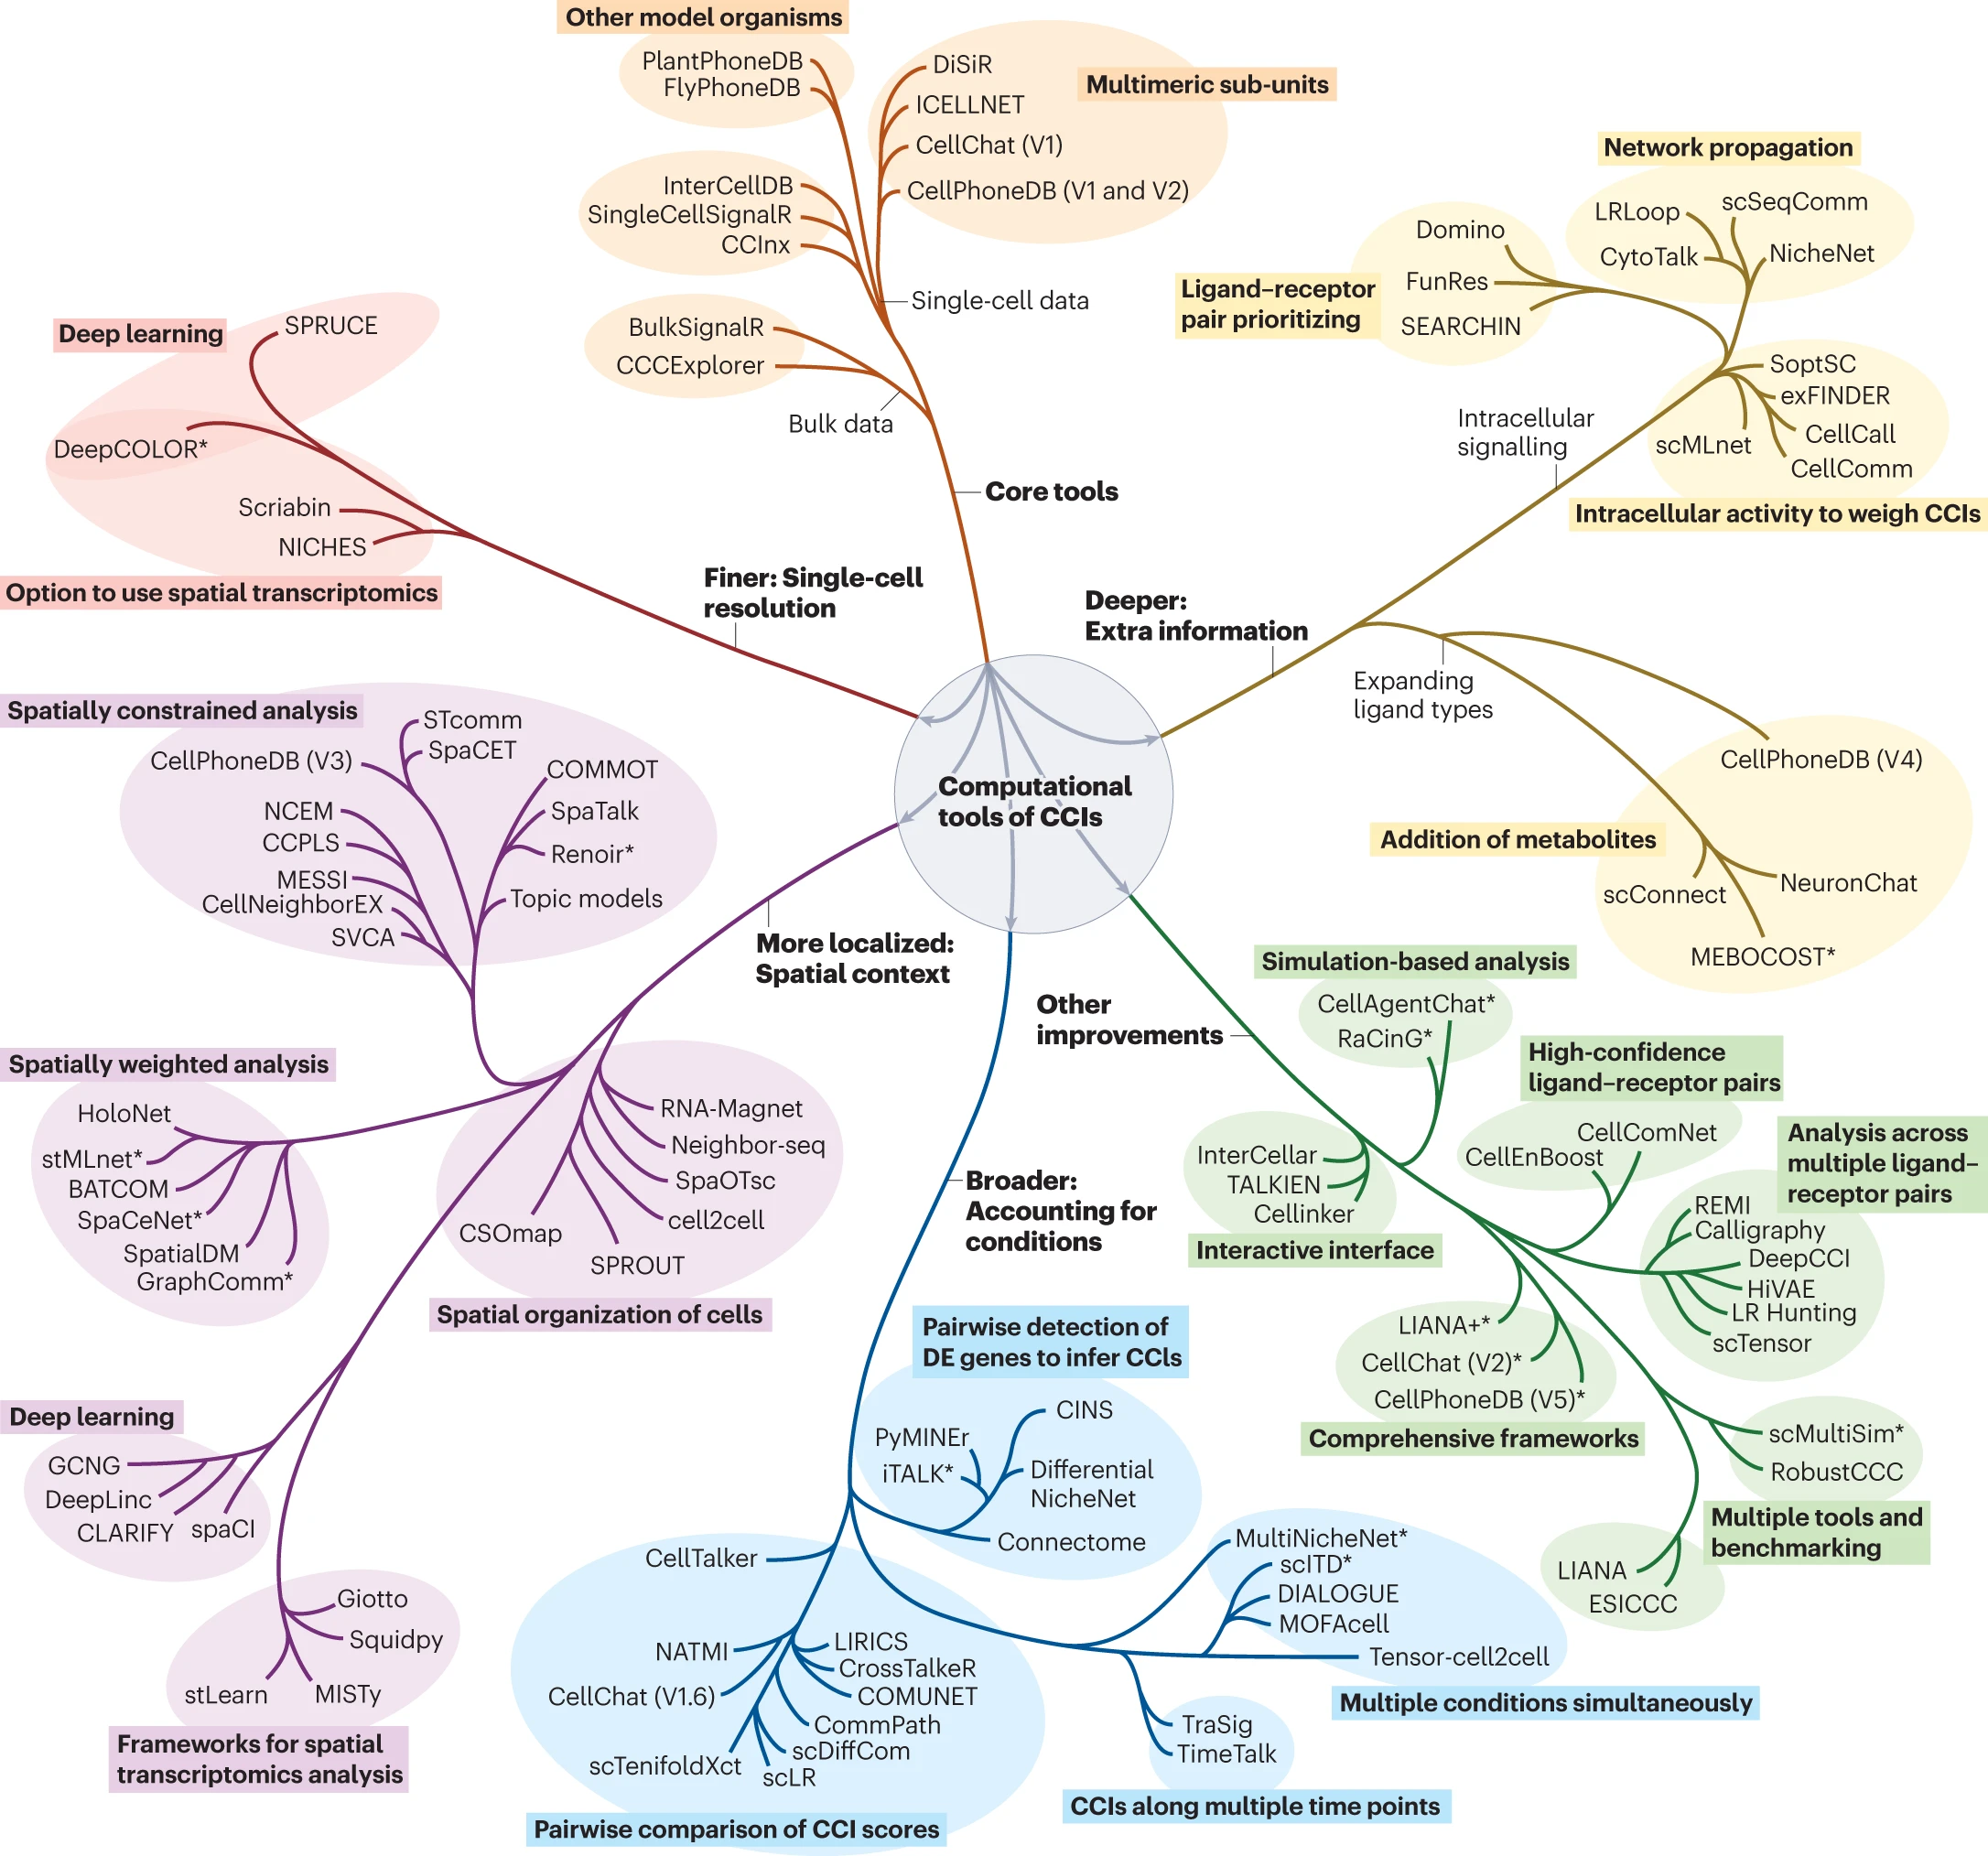
\includegraphics[width=0.85\linewidth,height=\textheight,keepaspectratio]{images/phylogenetic_tree_CCC.png}

}

\caption{\label{fig-phylo-CCC}Phylogenetic tree of computational tools
for inferring cell--cell interactions, from
\href{https://www.nature.com/articles/s41576-023-00685-8/figures/2}{\textcite{armingol2024nrg}}.
Tools published as a \textbf{preprint} are marked with an asterisk.}

\end{figure}%

Table~\ref{tbl-ccc-tools-intra} focuses on tools pairing
\textbf{intracellular signalling} and extra-cellular.

\global\setlength{\Oldarrayrulewidth}{\arrayrulewidth}

\global\setlength{\Oldtabcolsep}{\tabcolsep}

\setlength{\tabcolsep}{2pt}

\renewcommand*{\arraystretch}{1.5}



\providecommand{\ascline}[3]{\noalign{\global\arrayrulewidth #1}\arrayrulecolor[HTML]{#2}\cline{#3}}

\begin{longtable}[c]{ccccccccccccccccc}





\ascline{1.5pt}{666666}{1-17}

\multicolumn{1}{>{}l}{\textcolor[HTML]{000000}{\fontsize{11}{11}\selectfont{\global\setmainfont{Arial}{\textbf{Tool}}}}} & \multicolumn{1}{>{}l}{\textcolor[HTML]{000000}{\fontsize{11}{11}\selectfont{\global\setmainfont{Arial}{\textbf{Category}}}}} & \multicolumn{1}{>{}l}{\textcolor[HTML]{000000}{\fontsize{11}{11}\selectfont{\global\setmainfont{Arial}{\textbf{Method\ overview}}}}} & \multicolumn{1}{>{}l}{\textcolor[HTML]{000000}{\fontsize{11}{11}\selectfont{\global\setmainfont{Arial}{\textbf{Additional\ information}}}}} & \multicolumn{1}{>{}l}{\textcolor[HTML]{000000}{\fontsize{11}{11}\selectfont{\global\setmainfont{Arial}{\textbf{Tool\ classification}}}}} & \multicolumn{1}{>{}r}{\textcolor[HTML]{000000}{\fontsize{11}{11}\selectfont{\global\setmainfont{Arial}{\textbf{Intracellular}}}}} & \multicolumn{1}{>{}l}{\textcolor[HTML]{000000}{\fontsize{11}{11}\selectfont{\global\setmainfont{Arial}{\textbf{Language}}}}} & \multicolumn{1}{>{}l}{\textcolor[HTML]{000000}{\fontsize{11}{11}\selectfont{\global\setmainfont{Arial}{\textbf{Package}}}}} & \multicolumn{1}{>{}l}{\textcolor[HTML]{000000}{\fontsize{11}{11}\selectfont{\global\setmainfont{Arial}{\textbf{Refs}}}}} & \multicolumn{1}{>{}r}{\textcolor[HTML]{000000}{\fontsize{11}{11}\selectfont{\global\setmainfont{Arial}{\textbf{Year}}}}} & \multicolumn{1}{>{}r}{\textcolor[HTML]{000000}{\fontsize{11}{11}\selectfont{\global\setmainfont{Arial}{\textbf{Conditions}}}}} & \multicolumn{1}{>{}r}{\textcolor[HTML]{000000}{\fontsize{11}{11}\selectfont{\global\setmainfont{Arial}{\textbf{Spatial}}}}} & \multicolumn{1}{>{}r}{\textcolor[HTML]{000000}{\fontsize{11}{11}\selectfont{\global\setmainfont{Arial}{\textbf{Metabolites}}}}} & \multicolumn{1}{>{}r}{\textcolor[HTML]{000000}{\fontsize{11}{11}\selectfont{\global\setmainfont{Arial}{\textbf{Core\ Functions}}}}} & \multicolumn{1}{>{}r}{\textcolor[HTML]{000000}{\fontsize{11}{11}\selectfont{\global\setmainfont{Arial}{\textbf{Deep\ Learning}}}}} & \multicolumn{1}{>{}r}{\textcolor[HTML]{000000}{\fontsize{11}{11}\selectfont{\global\setmainfont{Arial}{\textbf{Classical\ Stats}}}}} & \multicolumn{1}{>{}r}{\textcolor[HTML]{000000}{\fontsize{11}{11}\selectfont{\global\setmainfont{Arial}{\textbf{Machine\ Learning}}}}} \\

\ascline{1.5pt}{666666}{1-17}\endfirsthead 

\ascline{1.5pt}{666666}{1-17}

\multicolumn{1}{>{}l}{\textcolor[HTML]{000000}{\fontsize{11}{11}\selectfont{\global\setmainfont{Arial}{\textbf{Tool}}}}} & \multicolumn{1}{>{}l}{\textcolor[HTML]{000000}{\fontsize{11}{11}\selectfont{\global\setmainfont{Arial}{\textbf{Category}}}}} & \multicolumn{1}{>{}l}{\textcolor[HTML]{000000}{\fontsize{11}{11}\selectfont{\global\setmainfont{Arial}{\textbf{Method\ overview}}}}} & \multicolumn{1}{>{}l}{\textcolor[HTML]{000000}{\fontsize{11}{11}\selectfont{\global\setmainfont{Arial}{\textbf{Additional\ information}}}}} & \multicolumn{1}{>{}l}{\textcolor[HTML]{000000}{\fontsize{11}{11}\selectfont{\global\setmainfont{Arial}{\textbf{Tool\ classification}}}}} & \multicolumn{1}{>{}r}{\textcolor[HTML]{000000}{\fontsize{11}{11}\selectfont{\global\setmainfont{Arial}{\textbf{Intracellular}}}}} & \multicolumn{1}{>{}l}{\textcolor[HTML]{000000}{\fontsize{11}{11}\selectfont{\global\setmainfont{Arial}{\textbf{Language}}}}} & \multicolumn{1}{>{}l}{\textcolor[HTML]{000000}{\fontsize{11}{11}\selectfont{\global\setmainfont{Arial}{\textbf{Package}}}}} & \multicolumn{1}{>{}l}{\textcolor[HTML]{000000}{\fontsize{11}{11}\selectfont{\global\setmainfont{Arial}{\textbf{Refs}}}}} & \multicolumn{1}{>{}r}{\textcolor[HTML]{000000}{\fontsize{11}{11}\selectfont{\global\setmainfont{Arial}{\textbf{Year}}}}} & \multicolumn{1}{>{}r}{\textcolor[HTML]{000000}{\fontsize{11}{11}\selectfont{\global\setmainfont{Arial}{\textbf{Conditions}}}}} & \multicolumn{1}{>{}r}{\textcolor[HTML]{000000}{\fontsize{11}{11}\selectfont{\global\setmainfont{Arial}{\textbf{Spatial}}}}} & \multicolumn{1}{>{}r}{\textcolor[HTML]{000000}{\fontsize{11}{11}\selectfont{\global\setmainfont{Arial}{\textbf{Metabolites}}}}} & \multicolumn{1}{>{}r}{\textcolor[HTML]{000000}{\fontsize{11}{11}\selectfont{\global\setmainfont{Arial}{\textbf{Core\ Functions}}}}} & \multicolumn{1}{>{}r}{\textcolor[HTML]{000000}{\fontsize{11}{11}\selectfont{\global\setmainfont{Arial}{\textbf{Deep\ Learning}}}}} & \multicolumn{1}{>{}r}{\textcolor[HTML]{000000}{\fontsize{11}{11}\selectfont{\global\setmainfont{Arial}{\textbf{Classical\ Stats}}}}} & \multicolumn{1}{>{}r}{\textcolor[HTML]{000000}{\fontsize{11}{11}\selectfont{\global\setmainfont{Arial}{\textbf{Machine\ Learning}}}}} \\

\ascline{1.5pt}{666666}{1-17}\endhead



\multicolumn{1}{>{}l}{\textcolor[HTML]{000000}{\fontsize{11}{11}\selectfont{\global\setmainfont{Arial}{MultiNicheNet}}}} & \multicolumn{1}{>{}l}{\textcolor[HTML]{000000}{\fontsize{11}{11}\selectfont{\global\setmainfont{Arial}{Broader:\ Accounting\ for\ multiple\ conditions}}}} & \multicolumn{1}{>{}l}{\textcolor[HTML]{000000}{\fontsize{11}{11}\selectfont{\global\setmainfont{Arial}{Prioritizes\ ligand-receptor\ pairs\ that\ are\ strongly\ expressed\ in\ the\ condition\ of\ interest,\ are\ cell-type\ specific,\ are\ present\ in\ most\ samples\ of\ the\ condition\ of\ interest,\ and\ whose\ target\ genes\ are\ enriched\ in\ the\ receiver\ cell\ type.\ It\ relies\ on\ edgeR\ analysis\ to\ score\ ligand-receptor\ pairs\ from\ differential\ expression\ and\ ligand\ activity.}}}} & \multicolumn{1}{>{}l}{\textcolor[HTML]{000000}{\fontsize{11}{11}\selectfont{\global\setmainfont{Arial}{Allows\ the\ study\ of\ between-\ and\ within-group\ differences.\ Batch\ and\ covariates\ variables\ can\ be\ added\ to\ the\ model\ to\ account\ for\ them\ when\ performing\ the\ DE\ analysis.}}}} & \multicolumn{1}{>{}l}{\textcolor[HTML]{000000}{\fontsize{11}{11}\selectfont{\global\setmainfont{Arial}{Data-driven}}}} & \multicolumn{1}{>{}r}{\textcolor[HTML]{000000}{\fontsize{11}{11}\selectfont{\global\setmainfont{Arial}{TRUE}}}} & \multicolumn{1}{>{}l}{\textcolor[HTML]{000000}{\fontsize{11}{11}\selectfont{\global\setmainfont{Arial}{R}}}} & \multicolumn{1}{>{}l}{\textcolor[HTML]{000000}{\fontsize{11}{11}\selectfont{\global\setmainfont{Arial}{https://github.com/saeyslab/multinichenetr}}}} & \multicolumn{1}{>{}l}{\textcolor[HTML]{000000}{\fontsize{11}{11}\selectfont{\global\setmainfont{Arial}{https://doi.org/10.1101/2023.06.13.544751}}}} & \multicolumn{1}{>{}r}{\textcolor[HTML]{000000}{\fontsize{11}{11}\selectfont{\global\setmainfont{Arial}{2,023}}}} & \multicolumn{1}{>{}r}{\textcolor[HTML]{000000}{\fontsize{11}{11}\selectfont{\global\setmainfont{Arial}{TRUE}}}} & \multicolumn{1}{>{}r}{\textcolor[HTML]{000000}{\fontsize{11}{11}\selectfont{\global\setmainfont{Arial}{FALSE}}}} & \multicolumn{1}{>{}r}{\textcolor[HTML]{000000}{\fontsize{11}{11}\selectfont{\global\setmainfont{Arial}{FALSE}}}} & \multicolumn{1}{>{}r}{\textcolor[HTML]{000000}{\fontsize{11}{11}\selectfont{\global\setmainfont{Arial}{TRUE}}}} & \multicolumn{1}{>{}r}{\textcolor[HTML]{000000}{\fontsize{11}{11}\selectfont{\global\setmainfont{Arial}{FALSE}}}} & \multicolumn{1}{>{}r}{\textcolor[HTML]{000000}{\fontsize{11}{11}\selectfont{\global\setmainfont{Arial}{TRUE}}}} & \multicolumn{1}{>{}r}{\textcolor[HTML]{000000}{\fontsize{11}{11}\selectfont{\global\setmainfont{Arial}{FALSE}}}} \\





\multicolumn{1}{>{}l}{\textcolor[HTML]{000000}{\fontsize{11}{11}\selectfont{\global\setmainfont{Arial}{TimeTalk}}}} & \multicolumn{1}{>{}l}{\textcolor[HTML]{000000}{\fontsize{11}{11}\selectfont{\global\setmainfont{Arial}{Broader:\ Accounting\ for\ multiple\ conditions}}}} & \multicolumn{1}{>{}l}{\textcolor[HTML]{000000}{\fontsize{11}{11}\selectfont{\global\setmainfont{Arial}{Designed\ for\ detecting\ CCIs\ in\ early\ embryo\ development.\ It\ computes\ a\ Spearman\ coefficient\ for\ LRIs\ between\ cell\ types\ along\ pseudotimes.\ Then,\ it\ computes\ a\ Granger's\ causality\ between\ the\ interaction\ score\ the\ co-varying\ LRI\ and\ the\ gene\ expression\ of\ their\ downstream\ master\ TFs.}}}} & \multicolumn{1}{>{}l}{\textcolor[HTML]{000000}{\fontsize{11}{11}\selectfont{\global\setmainfont{Arial}{This\ method\ prioritizes\ co-varying\ LRIs\ along\ pseudotimes\ that\ also\ form\ regulatory\ feedbacks\ with\ their\ downstream\ master\ TFs.}}}} & \multicolumn{1}{>{}l}{\textcolor[HTML]{000000}{\fontsize{11}{11}\selectfont{\global\setmainfont{Arial}{Data-driven}}}} & \multicolumn{1}{>{}r}{\textcolor[HTML]{000000}{\fontsize{11}{11}\selectfont{\global\setmainfont{Arial}{TRUE}}}} & \multicolumn{1}{>{}l}{\textcolor[HTML]{000000}{\fontsize{11}{11}\selectfont{\global\setmainfont{Arial}{R}}}} & \multicolumn{1}{>{}l}{\textcolor[HTML]{000000}{\fontsize{11}{11}\selectfont{\global\setmainfont{Arial}{https://github.com/ChengLiLab/TimeTalk}}}} & \multicolumn{1}{>{}l}{\textcolor[HTML]{000000}{\fontsize{11}{11}\selectfont{\global\setmainfont{Arial}{https://doi.org/10.1038/s42003-023-05283-2}}}} & \multicolumn{1}{>{}r}{\textcolor[HTML]{000000}{\fontsize{11}{11}\selectfont{\global\setmainfont{Arial}{2,023}}}} & \multicolumn{1}{>{}r}{\textcolor[HTML]{000000}{\fontsize{11}{11}\selectfont{\global\setmainfont{Arial}{TRUE}}}} & \multicolumn{1}{>{}r}{\textcolor[HTML]{000000}{\fontsize{11}{11}\selectfont{\global\setmainfont{Arial}{FALSE}}}} & \multicolumn{1}{>{}r}{\textcolor[HTML]{000000}{\fontsize{11}{11}\selectfont{\global\setmainfont{Arial}{FALSE}}}} & \multicolumn{1}{>{}r}{\textcolor[HTML]{000000}{\fontsize{11}{11}\selectfont{\global\setmainfont{Arial}{TRUE}}}} & \multicolumn{1}{>{}r}{\textcolor[HTML]{000000}{\fontsize{11}{11}\selectfont{\global\setmainfont{Arial}{FALSE}}}} & \multicolumn{1}{>{}r}{\textcolor[HTML]{000000}{\fontsize{11}{11}\selectfont{\global\setmainfont{Arial}{TRUE}}}} & \multicolumn{1}{>{}r}{\textcolor[HTML]{000000}{\fontsize{11}{11}\selectfont{\global\setmainfont{Arial}{FALSE}}}} \\





\multicolumn{1}{>{}l}{\textcolor[HTML]{000000}{\fontsize{11}{11}\selectfont{\global\setmainfont{Arial}{CommPath}}}} & \multicolumn{1}{>{}l}{\textcolor[HTML]{000000}{\fontsize{11}{11}\selectfont{\global\setmainfont{Arial}{Broader:\ Accounting\ for\ multiple\ conditions}}}} & \multicolumn{1}{>{}l}{\textcolor[HTML]{000000}{\fontsize{11}{11}\selectfont{\global\setmainfont{Arial}{Evaluates\ cell-cell\ communication\ chains,\ which\ corresponds\ to\ the\ effect\ that\ a\ receiver\ cell\ could\ have\ on\ a\ third\ cell.\ It\ uses\ CellA-CellB-CellC\ chain\ by\ weighting\ ligands\ from\ Cell\ A\ to\ receptors\ on\ Cell\ B,\ and\ ligand\ from\ Cell\ B\ to\ receptors\ on\ Cell\ C.\ Also\ evaluates\ the\ intracellular\ changes\ within\ Cell\ B\ connecting\ activity\ from\ Cell\ A\ to\ C.\ Identifies\ the\ differential\ activation\ of\ pathways\ between\ two\ conditions.}}}} & \multicolumn{1}{>{}l}{\textcolor[HTML]{000000}{\fontsize{11}{11}\selectfont{\global\setmainfont{Arial}{Performs\ pairwise\ comparisons\ between\ the\ CCC\ inferred\ for\ each\ condition\ separately.\ Also\ available\ in\ a\ web\ interface.}}}} & \multicolumn{1}{>{}l}{\textcolor[HTML]{000000}{\fontsize{11}{11}\selectfont{\global\setmainfont{Arial}{Data-driven}}}} & \multicolumn{1}{>{}r}{\textcolor[HTML]{000000}{\fontsize{11}{11}\selectfont{\global\setmainfont{Arial}{TRUE}}}} & \multicolumn{1}{>{}l}{\textcolor[HTML]{000000}{\fontsize{11}{11}\selectfont{\global\setmainfont{Arial}{R}}}} & \multicolumn{1}{>{}l}{\textcolor[HTML]{000000}{\fontsize{11}{11}\selectfont{\global\setmainfont{Arial}{https://github.com/yingyonghui/CommPath}}}} & \multicolumn{1}{>{}l}{\textcolor[HTML]{000000}{\fontsize{11}{11}\selectfont{\global\setmainfont{Arial}{https://doi.org/10.1016/j.csbj.2022.10.028}}}} & \multicolumn{1}{>{}r}{\textcolor[HTML]{000000}{\fontsize{11}{11}\selectfont{\global\setmainfont{Arial}{2,022}}}} & \multicolumn{1}{>{}r}{\textcolor[HTML]{000000}{\fontsize{11}{11}\selectfont{\global\setmainfont{Arial}{TRUE}}}} & \multicolumn{1}{>{}r}{\textcolor[HTML]{000000}{\fontsize{11}{11}\selectfont{\global\setmainfont{Arial}{FALSE}}}} & \multicolumn{1}{>{}r}{\textcolor[HTML]{000000}{\fontsize{11}{11}\selectfont{\global\setmainfont{Arial}{FALSE}}}} & \multicolumn{1}{>{}r}{\textcolor[HTML]{000000}{\fontsize{11}{11}\selectfont{\global\setmainfont{Arial}{TRUE}}}} & \multicolumn{1}{>{}r}{\textcolor[HTML]{000000}{\fontsize{11}{11}\selectfont{\global\setmainfont{Arial}{FALSE}}}} & \multicolumn{1}{>{}r}{\textcolor[HTML]{000000}{\fontsize{11}{11}\selectfont{\global\setmainfont{Arial}{FALSE}}}} & \multicolumn{1}{>{}r}{\textcolor[HTML]{000000}{\fontsize{11}{11}\selectfont{\global\setmainfont{Arial}{FALSE}}}} \\





\multicolumn{1}{>{}l}{\textcolor[HTML]{000000}{\fontsize{11}{11}\selectfont{\global\setmainfont{Arial}{DIALOGUE}}}} & \multicolumn{1}{>{}l}{\textcolor[HTML]{000000}{\fontsize{11}{11}\selectfont{\global\setmainfont{Arial}{Broader:\ Accounting\ for\ multiple\ conditions}}}} & \multicolumn{1}{>{}l}{\textcolor[HTML]{000000}{\fontsize{11}{11}\selectfont{\global\setmainfont{Arial}{Uses\ a\ matrix\ factorization\ method\ to\ identify\ MultiCellular\ Programs\ (MCPs)\ across\ multiple\ niches\ within\ the\ same\ tissue,\ or\ across\ multiple\ samples\ from\ different\ individuals.\ A\ MCP\ is\ captured\ per\ factor,\ and\ they\ can\ be\ integrated\ with\ ligand-receptor\ interactions\ to\ summarize\ communication\ represented\ by\ each\ MCP.}}}} & \multicolumn{1}{>{}l}{\textcolor[HTML]{000000}{\fontsize{11}{11}\selectfont{\global\setmainfont{Arial}{Detects\ factors\ or\ latent\ patterns\ of\ gene\ expression\ across\ multiple\ samples\ simultaneously,\ which\ can\ be\ used\ a\ posteriori\ to\ infer\ CCC.\ Dimensionality\ reduction\ method.}}}} & \multicolumn{1}{>{}l}{\textcolor[HTML]{000000}{\fontsize{11}{11}\selectfont{\global\setmainfont{Arial}{Data-driven}}}} & \multicolumn{1}{>{}r}{\textcolor[HTML]{000000}{\fontsize{11}{11}\selectfont{\global\setmainfont{Arial}{TRUE}}}} & \multicolumn{1}{>{}l}{\textcolor[HTML]{000000}{\fontsize{11}{11}\selectfont{\global\setmainfont{Arial}{R}}}} & \multicolumn{1}{>{}l}{\textcolor[HTML]{000000}{\fontsize{11}{11}\selectfont{\global\setmainfont{Arial}{https://github.com/livnatje/DIALOGUE}}}} & \multicolumn{1}{>{}l}{\textcolor[HTML]{000000}{\fontsize{11}{11}\selectfont{\global\setmainfont{Arial}{https://doi.org/10.1038/s41587-022-01288-0}}}} & \multicolumn{1}{>{}r}{\textcolor[HTML]{000000}{\fontsize{11}{11}\selectfont{\global\setmainfont{Arial}{2,022}}}} & \multicolumn{1}{>{}r}{\textcolor[HTML]{000000}{\fontsize{11}{11}\selectfont{\global\setmainfont{Arial}{TRUE}}}} & \multicolumn{1}{>{}r}{\textcolor[HTML]{000000}{\fontsize{11}{11}\selectfont{\global\setmainfont{Arial}{TRUE}}}} & \multicolumn{1}{>{}r}{\textcolor[HTML]{000000}{\fontsize{11}{11}\selectfont{\global\setmainfont{Arial}{FALSE}}}} & \multicolumn{1}{>{}r}{\textcolor[HTML]{000000}{\fontsize{11}{11}\selectfont{\global\setmainfont{Arial}{FALSE}}}} & \multicolumn{1}{>{}r}{\textcolor[HTML]{000000}{\fontsize{11}{11}\selectfont{\global\setmainfont{Arial}{FALSE}}}} & \multicolumn{1}{>{}r}{\textcolor[HTML]{000000}{\fontsize{11}{11}\selectfont{\global\setmainfont{Arial}{FALSE}}}} & \multicolumn{1}{>{}r}{\textcolor[HTML]{000000}{\fontsize{11}{11}\selectfont{\global\setmainfont{Arial}{TRUE}}}} \\





\multicolumn{1}{>{}l}{\textcolor[HTML]{000000}{\fontsize{11}{11}\selectfont{\global\setmainfont{Arial}{Differential\ NicheNet}}}} & \multicolumn{1}{>{}l}{\textcolor[HTML]{000000}{\fontsize{11}{11}\selectfont{\global\setmainfont{Arial}{Broader:\ Accounting\ for\ multiple\ conditions}}}} & \multicolumn{1}{>{}l}{\textcolor[HTML]{000000}{\fontsize{11}{11}\selectfont{\global\setmainfont{Arial}{Combines\ NicheNet\ with\ differential\ expression\ analysis\ between\ two\ conditions.\ This\ method\ returns\ a\ score\ that\ prioritizes\ up-regulation\ of\ the\ ligand\ and/or\ receptor\ in\ the\ condition\ of\ interest,\ expression\ level\ within\ the\ group,\ cell-type-specific\ expression,\ and\ high\ NicheNet\ score.}}}} & \multicolumn{1}{>{}l}{\textcolor[HTML]{000000}{\fontsize{11}{11}\selectfont{\global\setmainfont{Arial}{Performs\ pairwise\ comparisons\ between\ two\ conditions\ through\ a\ DE\ analysis.\ The\ method\ is\ powered\ by\ NicheNet.}}}} & \multicolumn{1}{>{}l}{\textcolor[HTML]{000000}{\fontsize{11}{11}\selectfont{\global\setmainfont{Arial}{Data-driven}}}} & \multicolumn{1}{>{}r}{\textcolor[HTML]{000000}{\fontsize{11}{11}\selectfont{\global\setmainfont{Arial}{TRUE}}}} & \multicolumn{1}{>{}l}{\textcolor[HTML]{000000}{\fontsize{11}{11}\selectfont{\global\setmainfont{Arial}{R}}}} & \multicolumn{1}{>{}l}{\textcolor[HTML]{000000}{\fontsize{11}{11}\selectfont{\global\setmainfont{Arial}{https://github.com/saeyslab/nichenetr/}}}} & \multicolumn{1}{>{}l}{\textcolor[HTML]{000000}{\fontsize{11}{11}\selectfont{\global\setmainfont{Arial}{https://doi.org/10.1016/j.cell.2021.12.018}}}} & \multicolumn{1}{>{}r}{\textcolor[HTML]{000000}{\fontsize{11}{11}\selectfont{\global\setmainfont{Arial}{2,022}}}} & \multicolumn{1}{>{}r}{\textcolor[HTML]{000000}{\fontsize{11}{11}\selectfont{\global\setmainfont{Arial}{TRUE}}}} & \multicolumn{1}{>{}r}{\textcolor[HTML]{000000}{\fontsize{11}{11}\selectfont{\global\setmainfont{Arial}{FALSE}}}} & \multicolumn{1}{>{}r}{\textcolor[HTML]{000000}{\fontsize{11}{11}\selectfont{\global\setmainfont{Arial}{FALSE}}}} & \multicolumn{1}{>{}r}{\textcolor[HTML]{000000}{\fontsize{11}{11}\selectfont{\global\setmainfont{Arial}{TRUE}}}} & \multicolumn{1}{>{}r}{\textcolor[HTML]{000000}{\fontsize{11}{11}\selectfont{\global\setmainfont{Arial}{FALSE}}}} & \multicolumn{1}{>{}r}{\textcolor[HTML]{000000}{\fontsize{11}{11}\selectfont{\global\setmainfont{Arial}{TRUE}}}} & \multicolumn{1}{>{}r}{\textcolor[HTML]{000000}{\fontsize{11}{11}\selectfont{\global\setmainfont{Arial}{TRUE}}}} \\





\multicolumn{1}{>{}l}{\textcolor[HTML]{000000}{\fontsize{11}{11}\selectfont{\global\setmainfont{Arial}{CellChat\ (V1.6)}}}} & \multicolumn{1}{>{}l}{\textcolor[HTML]{000000}{\fontsize{11}{11}\selectfont{\global\setmainfont{Arial}{Broader:\ Accounting\ for\ multiple\ conditions}}}} & \multicolumn{1}{>{}l}{\textcolor[HTML]{000000}{\fontsize{11}{11}\selectfont{\global\setmainfont{Arial}{Compares\ multiple\ cell-cell\ communication\ across\ multiple\ scRNA-seq\ datasets\ by\ leveraging\ CellChat\ V1.}}}} & \multicolumn{1}{>{}l}{\textcolor[HTML]{000000}{\fontsize{11}{11}\selectfont{\global\setmainfont{Arial}{Performs\ pairwise\ comparisons\ between\ the\ CCC\ inferred\ for\ each\ dataset\ separately.\ Integrates\ intracellular\ signaling\ as\ well\ to\ compute\ the\ communication\ scores.}}}} & \multicolumn{1}{>{}l}{\textcolor[HTML]{000000}{\fontsize{11}{11}\selectfont{\global\setmainfont{Arial}{Hybrid}}}} & \multicolumn{1}{>{}r}{\textcolor[HTML]{000000}{\fontsize{11}{11}\selectfont{\global\setmainfont{Arial}{TRUE}}}} & \multicolumn{1}{>{}l}{\textcolor[HTML]{000000}{\fontsize{11}{11}\selectfont{\global\setmainfont{Arial}{R}}}} & \multicolumn{1}{>{}l}{\textcolor[HTML]{000000}{\fontsize{11}{11}\selectfont{\global\setmainfont{Arial}{https://github.com/sqjin/CellChat}}}} & \multicolumn{1}{>{}l}{\textcolor[HTML]{000000}{\fontsize{11}{11}\selectfont{\global\setmainfont{Arial}{https://doi.org/10.3389/fgene.2021.751158}}}} & \multicolumn{1}{>{}r}{\textcolor[HTML]{000000}{\fontsize{11}{11}\selectfont{\global\setmainfont{Arial}{2,021}}}} & \multicolumn{1}{>{}r}{\textcolor[HTML]{000000}{\fontsize{11}{11}\selectfont{\global\setmainfont{Arial}{TRUE}}}} & \multicolumn{1}{>{}r}{\textcolor[HTML]{000000}{\fontsize{11}{11}\selectfont{\global\setmainfont{Arial}{FALSE}}}} & \multicolumn{1}{>{}r}{\textcolor[HTML]{000000}{\fontsize{11}{11}\selectfont{\global\setmainfont{Arial}{FALSE}}}} & \multicolumn{1}{>{}r}{\textcolor[HTML]{000000}{\fontsize{11}{11}\selectfont{\global\setmainfont{Arial}{TRUE}}}} & \multicolumn{1}{>{}r}{\textcolor[HTML]{000000}{\fontsize{11}{11}\selectfont{\global\setmainfont{Arial}{FALSE}}}} & \multicolumn{1}{>{}r}{\textcolor[HTML]{000000}{\fontsize{11}{11}\selectfont{\global\setmainfont{Arial}{TRUE}}}} & \multicolumn{1}{>{}r}{\textcolor[HTML]{000000}{\fontsize{11}{11}\selectfont{\global\setmainfont{Arial}{FALSE}}}} \\





\multicolumn{1}{>{}l}{\textcolor[HTML]{000000}{\fontsize{11}{11}\selectfont{\global\setmainfont{Arial}{BulkSignalR}}}} & \multicolumn{1}{>{}l}{\textcolor[HTML]{000000}{\fontsize{11}{11}\selectfont{\global\setmainfont{Arial}{Core\ Tool}}}} & \multicolumn{1}{>{}l}{\textcolor[HTML]{000000}{\fontsize{11}{11}\selectfont{\global\setmainfont{Arial}{Computes\ a\ Spearman\ correlation\ between\ ligands\ (L),\ and\ receptors\ (R),\ and\ another\ between\ receptors\ and\ target\ genes\ (T).\ To\ compute\ significance,\ relies\ on\ a\ null\ distribution\ of\ Spearman\ coefficients\ generated\ from\ randomized\ expression\ datasets.\ Assuming\ that\ distributions\ of\ LR\ and\ RT\ are\ independent,\ joint\ significance\ is\ the\ multiplication\ of\ their\ individual\ significances.}}}} & \multicolumn{1}{>{}l}{\textcolor[HTML]{000000}{\fontsize{11}{11}\selectfont{\global\setmainfont{Arial}{BulkSignalR\ can\ be\ applied\ to\ spatial\ transcriptomics\ with\ localized\ bulk\ data\ (e.g.,\ spots).\ Compares\ samples\ by\ standardizing\ the\ communication\ scores\ across\ samples.\ Employs\ a\ non-negative\ LASSO\ model\ to\ associate\ LRI\ with\ cell\ types.}}}} & \multicolumn{1}{>{}l}{\textcolor[HTML]{000000}{\fontsize{11}{11}\selectfont{\global\setmainfont{Arial}{Data-driven}}}} & \multicolumn{1}{>{}r}{\textcolor[HTML]{000000}{\fontsize{11}{11}\selectfont{\global\setmainfont{Arial}{TRUE}}}} & \multicolumn{1}{>{}l}{\textcolor[HTML]{000000}{\fontsize{11}{11}\selectfont{\global\setmainfont{Arial}{R}}}} & \multicolumn{1}{>{}l}{\textcolor[HTML]{000000}{\fontsize{11}{11}\selectfont{\global\setmainfont{Arial}{https://github.com/jcolinge/BulkSignalR}}}} & \multicolumn{1}{>{}l}{\textcolor[HTML]{000000}{\fontsize{11}{11}\selectfont{\global\setmainfont{Arial}{https://doi.org/10.1093/nar/gkad352}}}} & \multicolumn{1}{>{}r}{\textcolor[HTML]{000000}{\fontsize{11}{11}\selectfont{\global\setmainfont{Arial}{2,023}}}} & \multicolumn{1}{>{}r}{\textcolor[HTML]{000000}{\fontsize{11}{11}\selectfont{\global\setmainfont{Arial}{TRUE}}}} & \multicolumn{1}{>{}r}{\textcolor[HTML]{000000}{\fontsize{11}{11}\selectfont{\global\setmainfont{Arial}{TRUE}}}} & \multicolumn{1}{>{}r}{\textcolor[HTML]{000000}{\fontsize{11}{11}\selectfont{\global\setmainfont{Arial}{FALSE}}}} & \multicolumn{1}{>{}r}{\textcolor[HTML]{000000}{\fontsize{11}{11}\selectfont{\global\setmainfont{Arial}{TRUE}}}} & \multicolumn{1}{>{}r}{\textcolor[HTML]{000000}{\fontsize{11}{11}\selectfont{\global\setmainfont{Arial}{FALSE}}}} & \multicolumn{1}{>{}r}{\textcolor[HTML]{000000}{\fontsize{11}{11}\selectfont{\global\setmainfont{Arial}{TRUE}}}} & \multicolumn{1}{>{}r}{\textcolor[HTML]{000000}{\fontsize{11}{11}\selectfont{\global\setmainfont{Arial}{TRUE}}}} \\





\multicolumn{1}{>{}l}{\textcolor[HTML]{000000}{\fontsize{11}{11}\selectfont{\global\setmainfont{Arial}{CCCExplorer}}}} & \multicolumn{1}{>{}l}{\textcolor[HTML]{000000}{\fontsize{11}{11}\selectfont{\global\setmainfont{Arial}{Core\ Tool}}}} & \multicolumn{1}{>{}l}{\textcolor[HTML]{000000}{\fontsize{11}{11}\selectfont{\global\setmainfont{Arial}{Uses\ networks\ of\ ligand-receptor\ interactions\ connected\ to\ their\ TFs,\ and\ links\ the\ TFs\ with\ their\ target\ genes.\ CCCExplorer\ is\ based\ on\ differential\ expression\ of\ ligands\ and\ target\ genes\ (vs\ WT),\ while\ receptors\ and\ TFs\ are\ considered\ expressed\ if\ they\ are\ over\ a\ threshold.}}}} & \multicolumn{1}{>{}l}{\textcolor[HTML]{000000}{\fontsize{11}{11}\selectfont{\global\setmainfont{Arial}{Uses\ bulk\ RNA-seq\ data\ coming\ from\ multiple\ cell\ types\ separately.}}}} & \multicolumn{1}{>{}l}{\textcolor[HTML]{000000}{\fontsize{11}{11}\selectfont{\global\setmainfont{Arial}{Data-driven}}}} & \multicolumn{1}{>{}r}{\textcolor[HTML]{000000}{\fontsize{11}{11}\selectfont{\global\setmainfont{Arial}{TRUE}}}} & \multicolumn{1}{>{}l}{\textcolor[HTML]{000000}{\fontsize{11}{11}\selectfont{\global\setmainfont{Arial}{Standalone\ application}}}} & \multicolumn{1}{>{}l}{\textcolor[HTML]{000000}{\fontsize{11}{11}\selectfont{\global\setmainfont{Arial}{https://github.com/methodistsmab/CCCExplorer}}}} & \multicolumn{1}{>{}l}{\textcolor[HTML]{000000}{\fontsize{11}{11}\selectfont{\global\setmainfont{Arial}{https://doi.org/10.1016/j.celrep.2015.01.040}}}} & \multicolumn{1}{>{}r}{\textcolor[HTML]{000000}{\fontsize{11}{11}\selectfont{\global\setmainfont{Arial}{2,015}}}} & \multicolumn{1}{>{}r}{\textcolor[HTML]{000000}{\fontsize{11}{11}\selectfont{\global\setmainfont{Arial}{TRUE}}}} & \multicolumn{1}{>{}r}{\textcolor[HTML]{000000}{\fontsize{11}{11}\selectfont{\global\setmainfont{Arial}{FALSE}}}} & \multicolumn{1}{>{}r}{\textcolor[HTML]{000000}{\fontsize{11}{11}\selectfont{\global\setmainfont{Arial}{FALSE}}}} & \multicolumn{1}{>{}r}{\textcolor[HTML]{000000}{\fontsize{11}{11}\selectfont{\global\setmainfont{Arial}{TRUE}}}} & \multicolumn{1}{>{}r}{\textcolor[HTML]{000000}{\fontsize{11}{11}\selectfont{\global\setmainfont{Arial}{FALSE}}}} & \multicolumn{1}{>{}r}{\textcolor[HTML]{000000}{\fontsize{11}{11}\selectfont{\global\setmainfont{Arial}{TRUE}}}} & \multicolumn{1}{>{}r}{\textcolor[HTML]{000000}{\fontsize{11}{11}\selectfont{\global\setmainfont{Arial}{FALSE}}}} \\





\multicolumn{1}{>{}l}{\textcolor[HTML]{000000}{\fontsize{11}{11}\selectfont{\global\setmainfont{Arial}{PlantPhoneDB}}}} & \multicolumn{1}{>{}l}{\textcolor[HTML]{000000}{\fontsize{11}{11}\selectfont{\global\setmainfont{Arial}{Core\ Tool}}}} & \multicolumn{1}{>{}l}{\textcolor[HTML]{000000}{\fontsize{11}{11}\selectfont{\global\setmainfont{Arial}{Implements\ multiple\ communication\ scores,\ including\ a\ regularized\ product,\ weight\ product,\ mean,\ and\ product\ of\ gene\ expression\ between\ the\ ligand\ and\ the\ receptor\ in\ a\ pair\ of\ cell\ types.\ Uses\ target\ genes\ of\ the\ receptors\ to\ inspect\ intracellular\ signaling.\ For\ target\ genes,\ it\ uses\ differential\ expression\ analysis.}}}} & \multicolumn{1}{>{}l}{\textcolor[HTML]{000000}{\fontsize{11}{11}\selectfont{\global\setmainfont{Arial}{It\ performs\ permutations\ to\ select\ significant\ interactions.\ Intended\ for\ studying\ 5\ different\ species\ of\ plants.}}}} & \multicolumn{1}{>{}l}{\textcolor[HTML]{000000}{\fontsize{11}{11}\selectfont{\global\setmainfont{Arial}{Hybrid}}}} & \multicolumn{1}{>{}r}{\textcolor[HTML]{000000}{\fontsize{11}{11}\selectfont{\global\setmainfont{Arial}{TRUE}}}} & \multicolumn{1}{>{}l}{\textcolor[HTML]{000000}{\fontsize{11}{11}\selectfont{\global\setmainfont{Arial}{R}}}} & \multicolumn{1}{>{}l}{\textcolor[HTML]{000000}{\fontsize{11}{11}\selectfont{\global\setmainfont{Arial}{https://github.com/Jasonxu0109/PlantPhoneDB}}}} & \multicolumn{1}{>{}l}{\textcolor[HTML]{000000}{\fontsize{11}{11}\selectfont{\global\setmainfont{Arial}{https://doi.org/10.1111/pbi.13893}}}} & \multicolumn{1}{>{}r}{\textcolor[HTML]{000000}{\fontsize{11}{11}\selectfont{\global\setmainfont{Arial}{2,022}}}} & \multicolumn{1}{>{}r}{\textcolor[HTML]{000000}{\fontsize{11}{11}\selectfont{\global\setmainfont{Arial}{FALSE}}}} & \multicolumn{1}{>{}r}{\textcolor[HTML]{000000}{\fontsize{11}{11}\selectfont{\global\setmainfont{Arial}{FALSE}}}} & \multicolumn{1}{>{}r}{\textcolor[HTML]{000000}{\fontsize{11}{11}\selectfont{\global\setmainfont{Arial}{FALSE}}}} & \multicolumn{1}{>{}r}{\textcolor[HTML]{000000}{\fontsize{11}{11}\selectfont{\global\setmainfont{Arial}{TRUE}}}} & \multicolumn{1}{>{}r}{\textcolor[HTML]{000000}{\fontsize{11}{11}\selectfont{\global\setmainfont{Arial}{FALSE}}}} & \multicolumn{1}{>{}r}{\textcolor[HTML]{000000}{\fontsize{11}{11}\selectfont{\global\setmainfont{Arial}{TRUE}}}} & \multicolumn{1}{>{}r}{\textcolor[HTML]{000000}{\fontsize{11}{11}\selectfont{\global\setmainfont{Arial}{FALSE}}}} \\





\multicolumn{1}{>{}l}{\textcolor[HTML]{000000}{\fontsize{11}{11}\selectfont{\global\setmainfont{Arial}{LRLoop}}}} & \multicolumn{1}{>{}l}{\textcolor[HTML]{000000}{\fontsize{11}{11}\selectfont{\global\setmainfont{Arial}{Deeper:\ New\ ligand\ types\ and\ intracellular\ signaling}}}} & \multicolumn{1}{>{}l}{\textcolor[HTML]{000000}{\fontsize{11}{11}\selectfont{\global\setmainfont{Arial}{Builds\ upon\ NicheNet\ to\ compute\ the\ regulatory\ potential\ between\ receptors\ and\ target\ genes,\ instead\ of\ ligands\ and\ target\ genes.\ By\ using\ a\ Personalized\ PageRank\ to\ compute\ that\ potential,\ it\ is\ able\ to\ detect\ responsive\ ligands\ and\ receptors,\ connected\ through\ the\ intracellular\ signaling\ information.\ Thus,\ LRLoop\ detects\ [L1–R1]<->[L2–R2]\ interactions\ where\ L1\ and\ L2\ are\ ligands\ that\ are\ among\ the\ target\ genes\ of\ R2\ and\ R1\ receptors,\ respectively.}}}} & \multicolumn{1}{>{}l}{\textcolor[HTML]{000000}{\fontsize{11}{11}\selectfont{\global\setmainfont{Arial}{LRLoop\ prioritizes\ bi-directional\ ligand–receptor\ interactions\ forming\ a\ closed\ feedback\ loop.}}}} & \multicolumn{1}{>{}l}{\textcolor[HTML]{000000}{\fontsize{11}{11}\selectfont{\global\setmainfont{Arial}{Data-driven}}}} & \multicolumn{1}{>{}r}{\textcolor[HTML]{000000}{\fontsize{11}{11}\selectfont{\global\setmainfont{Arial}{TRUE}}}} & \multicolumn{1}{>{}l}{\textcolor[HTML]{000000}{\fontsize{11}{11}\selectfont{\global\setmainfont{Arial}{R}}}} & \multicolumn{1}{>{}l}{\textcolor[HTML]{000000}{\fontsize{11}{11}\selectfont{\global\setmainfont{Arial}{https://github.com/Pinlyu3/LRLoop}}}} & \multicolumn{1}{>{}l}{\textcolor[HTML]{000000}{\fontsize{11}{11}\selectfont{\global\setmainfont{Arial}{https://doi.org/10.1093/bioinformatics/btac447}}}} & \multicolumn{1}{>{}r}{\textcolor[HTML]{000000}{\fontsize{11}{11}\selectfont{\global\setmainfont{Arial}{2,022}}}} & \multicolumn{1}{>{}r}{\textcolor[HTML]{000000}{\fontsize{11}{11}\selectfont{\global\setmainfont{Arial}{TRUE}}}} & \multicolumn{1}{>{}r}{\textcolor[HTML]{000000}{\fontsize{11}{11}\selectfont{\global\setmainfont{Arial}{FALSE}}}} & \multicolumn{1}{>{}r}{\textcolor[HTML]{000000}{\fontsize{11}{11}\selectfont{\global\setmainfont{Arial}{FALSE}}}} & \multicolumn{1}{>{}r}{\textcolor[HTML]{000000}{\fontsize{11}{11}\selectfont{\global\setmainfont{Arial}{FALSE}}}} & \multicolumn{1}{>{}r}{\textcolor[HTML]{000000}{\fontsize{11}{11}\selectfont{\global\setmainfont{Arial}{FALSE}}}} & \multicolumn{1}{>{}r}{\textcolor[HTML]{000000}{\fontsize{11}{11}\selectfont{\global\setmainfont{Arial}{FALSE}}}} & \multicolumn{1}{>{}r}{\textcolor[HTML]{000000}{\fontsize{11}{11}\selectfont{\global\setmainfont{Arial}{TRUE}}}} \\





\multicolumn{1}{>{}l}{\textcolor[HTML]{000000}{\fontsize{11}{11}\selectfont{\global\setmainfont{Arial}{scSeqComm}}}} & \multicolumn{1}{>{}l}{\textcolor[HTML]{000000}{\fontsize{11}{11}\selectfont{\global\setmainfont{Arial}{Deeper:\ New\ ligand\ types\ and\ intracellular\ signaling}}}} & \multicolumn{1}{>{}l}{\textcolor[HTML]{000000}{\fontsize{11}{11}\selectfont{\global\setmainfont{Arial}{Predicts\ communication\ scores\ by\ selecting\ the\ minimum\ expression\ between\ a\ ligand\ and\ a\ receptor.\ It\ incorporates\ intracellular\ signaling\ by\ assigning\ scores\ to\ receptor-TF\ associations\ using\ a\ Personalized\ PageRank\ algorithm.\ It\ also\ includes\ TF\ activity\ on\ the\ final\ score.}}}} & \multicolumn{1}{>{}l}{\textcolor[HTML]{000000}{\fontsize{11}{11}\selectfont{\global\setmainfont{Arial}{It\ performs\ permutations\ to\ select\ significant\ interactions.}}}} & \multicolumn{1}{>{}l}{\textcolor[HTML]{000000}{\fontsize{11}{11}\selectfont{\global\setmainfont{Arial}{Data-driven}}}} & \multicolumn{1}{>{}r}{\textcolor[HTML]{000000}{\fontsize{11}{11}\selectfont{\global\setmainfont{Arial}{TRUE}}}} & \multicolumn{1}{>{}l}{\textcolor[HTML]{000000}{\fontsize{11}{11}\selectfont{\global\setmainfont{Arial}{R}}}} & \multicolumn{1}{>{}l}{\textcolor[HTML]{000000}{\fontsize{11}{11}\selectfont{\global\setmainfont{Arial}{https://gitlab.com/sysbiobig/scseqcomm}}}} & \multicolumn{1}{>{}l}{\textcolor[HTML]{000000}{\fontsize{11}{11}\selectfont{\global\setmainfont{Arial}{https://doi.org/10.1093/bioinformatics/btac036}}}} & \multicolumn{1}{>{}r}{\textcolor[HTML]{000000}{\fontsize{11}{11}\selectfont{\global\setmainfont{Arial}{2,022}}}} & \multicolumn{1}{>{}r}{\textcolor[HTML]{000000}{\fontsize{11}{11}\selectfont{\global\setmainfont{Arial}{FALSE}}}} & \multicolumn{1}{>{}r}{\textcolor[HTML]{000000}{\fontsize{11}{11}\selectfont{\global\setmainfont{Arial}{TRUE}}}} & \multicolumn{1}{>{}r}{\textcolor[HTML]{000000}{\fontsize{11}{11}\selectfont{\global\setmainfont{Arial}{FALSE}}}} & \multicolumn{1}{>{}r}{\textcolor[HTML]{000000}{\fontsize{11}{11}\selectfont{\global\setmainfont{Arial}{FALSE}}}} & \multicolumn{1}{>{}r}{\textcolor[HTML]{000000}{\fontsize{11}{11}\selectfont{\global\setmainfont{Arial}{FALSE}}}} & \multicolumn{1}{>{}r}{\textcolor[HTML]{000000}{\fontsize{11}{11}\selectfont{\global\setmainfont{Arial}{TRUE}}}} & \multicolumn{1}{>{}r}{\textcolor[HTML]{000000}{\fontsize{11}{11}\selectfont{\global\setmainfont{Arial}{TRUE}}}} \\





\multicolumn{1}{>{}l}{\textcolor[HTML]{000000}{\fontsize{11}{11}\selectfont{\global\setmainfont{Arial}{CytoTalk}}}} & \multicolumn{1}{>{}l}{\textcolor[HTML]{000000}{\fontsize{11}{11}\selectfont{\global\setmainfont{Arial}{Deeper:\ New\ ligand\ types\ and\ intracellular\ signaling}}}} & \multicolumn{1}{>{}l}{\textcolor[HTML]{000000}{\fontsize{11}{11}\selectfont{\global\setmainfont{Arial}{Connects\ two\ intracellular\ networks\ (from\ different\ cells)\ through\ known\ ligand-receptor\ interactions.\ It\ prioritizes\ LR\ pairs\ that\ are\ not\ used\ for\ autocrine\ interactions\ (low\ correlation\ within\ the\ same\ cluster)\ to\ assign\ a\ high\ crosstalk\ score.\ Then,\ it\ employs\ a\ network\ propagation\ based\ on\ the\ gene\ expression\ of\ intracellular\ genes.\ Finally\ it\ identifies\ signaling\ networks\ as\ a\ prize-collecting\ steiner\ forest\ problem\ to\ find\ intracellular\ genes\ that\ are\ close\ to\ highly-scored\ LR\ pairs.}}}} & \multicolumn{1}{>{}l}{\textcolor[HTML]{000000}{\fontsize{11}{11}\selectfont{\global\setmainfont{Arial}{Employs\ a\ degree-preserving\ network\ permutation\ to\ reduce\ false\ positives.}}}} & \multicolumn{1}{>{}l}{\textcolor[HTML]{000000}{\fontsize{11}{11}\selectfont{\global\setmainfont{Arial}{Data-driven}}}} & \multicolumn{1}{>{}r}{\textcolor[HTML]{000000}{\fontsize{11}{11}\selectfont{\global\setmainfont{Arial}{TRUE}}}} & \multicolumn{1}{>{}l}{\textcolor[HTML]{000000}{\fontsize{11}{11}\selectfont{\global\setmainfont{Arial}{R}}}} & \multicolumn{1}{>{}l}{\textcolor[HTML]{000000}{\fontsize{11}{11}\selectfont{\global\setmainfont{Arial}{https://github.com/tanlabcode/CytoTalk}}}} & \multicolumn{1}{>{}l}{\textcolor[HTML]{000000}{\fontsize{11}{11}\selectfont{\global\setmainfont{Arial}{https://doi.org/10.1126/sciadv.abf1356}}}} & \multicolumn{1}{>{}r}{\textcolor[HTML]{000000}{\fontsize{11}{11}\selectfont{\global\setmainfont{Arial}{2,021}}}} & \multicolumn{1}{>{}r}{\textcolor[HTML]{000000}{\fontsize{11}{11}\selectfont{\global\setmainfont{Arial}{FALSE}}}} & \multicolumn{1}{>{}r}{\textcolor[HTML]{000000}{\fontsize{11}{11}\selectfont{\global\setmainfont{Arial}{FALSE}}}} & \multicolumn{1}{>{}r}{\textcolor[HTML]{000000}{\fontsize{11}{11}\selectfont{\global\setmainfont{Arial}{FALSE}}}} & \multicolumn{1}{>{}r}{\textcolor[HTML]{000000}{\fontsize{11}{11}\selectfont{\global\setmainfont{Arial}{FALSE}}}} & \multicolumn{1}{>{}r}{\textcolor[HTML]{000000}{\fontsize{11}{11}\selectfont{\global\setmainfont{Arial}{FALSE}}}} & \multicolumn{1}{>{}r}{\textcolor[HTML]{000000}{\fontsize{11}{11}\selectfont{\global\setmainfont{Arial}{TRUE}}}} & \multicolumn{1}{>{}r}{\textcolor[HTML]{000000}{\fontsize{11}{11}\selectfont{\global\setmainfont{Arial}{FALSE}}}} \\





\multicolumn{1}{>{}l}{\textcolor[HTML]{000000}{\fontsize{11}{11}\selectfont{\global\setmainfont{Arial}{Domino}}}} & \multicolumn{1}{>{}l}{\textcolor[HTML]{000000}{\fontsize{11}{11}\selectfont{\global\setmainfont{Arial}{Deeper:\ New\ ligand\ types\ and\ intracellular\ signaling}}}} & \multicolumn{1}{>{}l}{\textcolor[HTML]{000000}{\fontsize{11}{11}\selectfont{\global\setmainfont{Arial}{Uses\ a\ network\ of\ ligand-receptor-TF-targets,\ and\ considers\ only\ pathways\ whose\ ligands\ and\ receptors\ are\ expressed.\ This\ means\ that\ they\ are\ over\ a\ z-value\ when\ comparing\ all\ clusters\ or\ cell\ types.\ It\ connects\ receptors\ to\ TF\ using\ Pearson\ correlation.\ It\ excludes\ receptors\ that\ are\ downstream\ to\ a\ TF\ in\ the\ network.}}}} & \multicolumn{1}{>{}l}{\textcolor[HTML]{000000}{\fontsize{11}{11}\selectfont{\global\setmainfont{Arial}{Domino\ is\ able\ to\ compare\ two\ conditions.\ Also,\ it\ can\ extract\ condition-specific\ signaling.}}}} & \multicolumn{1}{>{}l}{\textcolor[HTML]{000000}{\fontsize{11}{11}\selectfont{\global\setmainfont{Arial}{Data-driven}}}} & \multicolumn{1}{>{}r}{\textcolor[HTML]{000000}{\fontsize{11}{11}\selectfont{\global\setmainfont{Arial}{TRUE}}}} & \multicolumn{1}{>{}l}{\textcolor[HTML]{000000}{\fontsize{11}{11}\selectfont{\global\setmainfont{Arial}{R}}}} & \multicolumn{1}{>{}l}{\textcolor[HTML]{000000}{\fontsize{11}{11}\selectfont{\global\setmainfont{Arial}{https://github.com/chris-cherry/domino}}}} & \multicolumn{1}{>{}l}{\textcolor[HTML]{000000}{\fontsize{11}{11}\selectfont{\global\setmainfont{Arial}{https://doi.org/10.1038/s41551-021-00770-5}}}} & \multicolumn{1}{>{}r}{\textcolor[HTML]{000000}{\fontsize{11}{11}\selectfont{\global\setmainfont{Arial}{2,021}}}} & \multicolumn{1}{>{}r}{\textcolor[HTML]{000000}{\fontsize{11}{11}\selectfont{\global\setmainfont{Arial}{TRUE}}}} & \multicolumn{1}{>{}r}{\textcolor[HTML]{000000}{\fontsize{11}{11}\selectfont{\global\setmainfont{Arial}{FALSE}}}} & \multicolumn{1}{>{}r}{\textcolor[HTML]{000000}{\fontsize{11}{11}\selectfont{\global\setmainfont{Arial}{FALSE}}}} & \multicolumn{1}{>{}r}{\textcolor[HTML]{000000}{\fontsize{11}{11}\selectfont{\global\setmainfont{Arial}{FALSE}}}} & \multicolumn{1}{>{}r}{\textcolor[HTML]{000000}{\fontsize{11}{11}\selectfont{\global\setmainfont{Arial}{FALSE}}}} & \multicolumn{1}{>{}r}{\textcolor[HTML]{000000}{\fontsize{11}{11}\selectfont{\global\setmainfont{Arial}{TRUE}}}} & \multicolumn{1}{>{}r}{\textcolor[HTML]{000000}{\fontsize{11}{11}\selectfont{\global\setmainfont{Arial}{FALSE}}}} \\





\multicolumn{1}{>{}l}{\textcolor[HTML]{000000}{\fontsize{11}{11}\selectfont{\global\setmainfont{Arial}{FunRes}}}} & \multicolumn{1}{>{}l}{\textcolor[HTML]{000000}{\fontsize{11}{11}\selectfont{\global\setmainfont{Arial}{Deeper:\ New\ ligand\ types\ and\ intracellular\ signaling}}}} & \multicolumn{1}{>{}l}{\textcolor[HTML]{000000}{\fontsize{11}{11}\selectfont{\global\setmainfont{Arial}{Binary\ presence\ of\ TFs\ by\ fraction\ of\ cells\ within\ a\ cluster.\ It\ uses\ a\ Markov\ Chain\ model\ to\ infer\ the\ probability\ of\ a\ receptor\ to\ induce\ present\ TFs,\ considering\ intermediate\ genes.\ Finally\ computes\ LR\ score\ as\ the\ product\ of\ the\ average\ expression\ of\ the\ ligand\ and\ the\ receptor\ in\ their\ respective\ populations\ (only\ applies\ for\ ligands\ and\ receptors\ selected\ in\ a\ CCI\ scaffold)}}}} & \multicolumn{1}{>{}l}{\textcolor[HTML]{000000}{\fontsize{11}{11}\selectfont{\global\setmainfont{Arial}{FunRes\ builds\ a\ CCI\ network\ from\ LR\ pairs\ with\ significantly\ higher\ score\ compared\ to\ other\ interactions\ in\ the\ interaction\ scaffold.}}}} & \multicolumn{1}{>{}l}{\textcolor[HTML]{000000}{\fontsize{11}{11}\selectfont{\global\setmainfont{Arial}{Data-driven}}}} & \multicolumn{1}{>{}r}{\textcolor[HTML]{000000}{\fontsize{11}{11}\selectfont{\global\setmainfont{Arial}{TRUE}}}} & \multicolumn{1}{>{}l}{\textcolor[HTML]{000000}{\fontsize{11}{11}\selectfont{\global\setmainfont{Arial}{R}}}} & \multicolumn{1}{>{}l}{\textcolor[HTML]{000000}{\fontsize{11}{11}\selectfont{\global\setmainfont{Arial}{https://git-r3lab.uni.lu/kartikeya.singh/funres}}}} & \multicolumn{1}{>{}l}{\textcolor[HTML]{000000}{\fontsize{11}{11}\selectfont{\global\setmainfont{Arial}{https://doi.org/10.1093/bib/bbaa283}}}} & \multicolumn{1}{>{}r}{\textcolor[HTML]{000000}{\fontsize{11}{11}\selectfont{\global\setmainfont{Arial}{2,021}}}} & \multicolumn{1}{>{}r}{\textcolor[HTML]{000000}{\fontsize{11}{11}\selectfont{\global\setmainfont{Arial}{FALSE}}}} & \multicolumn{1}{>{}r}{\textcolor[HTML]{000000}{\fontsize{11}{11}\selectfont{\global\setmainfont{Arial}{FALSE}}}} & \multicolumn{1}{>{}r}{\textcolor[HTML]{000000}{\fontsize{11}{11}\selectfont{\global\setmainfont{Arial}{FALSE}}}} & \multicolumn{1}{>{}r}{\textcolor[HTML]{000000}{\fontsize{11}{11}\selectfont{\global\setmainfont{Arial}{TRUE}}}} & \multicolumn{1}{>{}r}{\textcolor[HTML]{000000}{\fontsize{11}{11}\selectfont{\global\setmainfont{Arial}{FALSE}}}} & \multicolumn{1}{>{}r}{\textcolor[HTML]{000000}{\fontsize{11}{11}\selectfont{\global\setmainfont{Arial}{TRUE}}}} & \multicolumn{1}{>{}r}{\textcolor[HTML]{000000}{\fontsize{11}{11}\selectfont{\global\setmainfont{Arial}{TRUE}}}} \\





\multicolumn{1}{>{}l}{\textcolor[HTML]{000000}{\fontsize{11}{11}\selectfont{\global\setmainfont{Arial}{scMLnet}}}} & \multicolumn{1}{>{}l}{\textcolor[HTML]{000000}{\fontsize{11}{11}\selectfont{\global\setmainfont{Arial}{Deeper:\ New\ ligand\ types\ and\ intracellular\ signaling}}}} & \multicolumn{1}{>{}l}{\textcolor[HTML]{000000}{\fontsize{11}{11}\selectfont{\global\setmainfont{Arial}{Builds\ a\ multilayer\ network\ of\ Ligand-Receptor\ pairs,\ Receptor-TF\ pathways,\ and\ TF-target\ genes.\ It\ uses\ the\ cell-type-specific\ highly-expressed\ genes\ to\ infer\ CCIs.\ LR\ pairs\ are\ scored\ with\ their\ expression\ product.\ It\ uses\ Fisher's\ exact\ test\ to\ consider\ active\ TFs,\ by\ using\ information\ of\ expressed\ target\ genes.\ Then\ LR\ pairs\ and\ enriched\ TFs\ are\ connected\ with\ another\ Fisher's\ test,\ considering\ whether\ active\ TFs\ are\ enriched\ in\ a\ given\ receptor.\ Thus,\ only\ LR\ pairs\ passing\ these\ test\ are\ retained.}}}} & \multicolumn{1}{>{}l}{\textcolor[HTML]{000000}{\fontsize{11}{11}\selectfont{\global\setmainfont{Arial}{Method\ based\ on\ multilayer\ networks.}}}} & \multicolumn{1}{>{}l}{\textcolor[HTML]{000000}{\fontsize{11}{11}\selectfont{\global\setmainfont{Arial}{Data-driven}}}} & \multicolumn{1}{>{}r}{\textcolor[HTML]{000000}{\fontsize{11}{11}\selectfont{\global\setmainfont{Arial}{TRUE}}}} & \multicolumn{1}{>{}l}{\textcolor[HTML]{000000}{\fontsize{11}{11}\selectfont{\global\setmainfont{Arial}{R}}}} & \multicolumn{1}{>{}l}{\textcolor[HTML]{000000}{\fontsize{11}{11}\selectfont{\global\setmainfont{Arial}{https://github.com/SunXQlab/scMLnet}}}} & \multicolumn{1}{>{}l}{\textcolor[HTML]{000000}{\fontsize{11}{11}\selectfont{\global\setmainfont{Arial}{https://doi.org/10.1093/bib/bbaa327}}}} & \multicolumn{1}{>{}r}{\textcolor[HTML]{000000}{\fontsize{11}{11}\selectfont{\global\setmainfont{Arial}{2,020}}}} & \multicolumn{1}{>{}r}{\textcolor[HTML]{000000}{\fontsize{11}{11}\selectfont{\global\setmainfont{Arial}{FALSE}}}} & \multicolumn{1}{>{}r}{\textcolor[HTML]{000000}{\fontsize{11}{11}\selectfont{\global\setmainfont{Arial}{FALSE}}}} & \multicolumn{1}{>{}r}{\textcolor[HTML]{000000}{\fontsize{11}{11}\selectfont{\global\setmainfont{Arial}{FALSE}}}} & \multicolumn{1}{>{}r}{\textcolor[HTML]{000000}{\fontsize{11}{11}\selectfont{\global\setmainfont{Arial}{TRUE}}}} & \multicolumn{1}{>{}r}{\textcolor[HTML]{000000}{\fontsize{11}{11}\selectfont{\global\setmainfont{Arial}{FALSE}}}} & \multicolumn{1}{>{}r}{\textcolor[HTML]{000000}{\fontsize{11}{11}\selectfont{\global\setmainfont{Arial}{TRUE}}}} & \multicolumn{1}{>{}r}{\textcolor[HTML]{000000}{\fontsize{11}{11}\selectfont{\global\setmainfont{Arial}{FALSE}}}} \\





\multicolumn{1}{>{}l}{\textcolor[HTML]{000000}{\fontsize{11}{11}\selectfont{\global\setmainfont{Arial}{SEARCHIN}}}} & \multicolumn{1}{>{}l}{\textcolor[HTML]{000000}{\fontsize{11}{11}\selectfont{\global\setmainfont{Arial}{Deeper:\ New\ ligand\ types\ and\ intracellular\ signaling}}}} & \multicolumn{1}{>{}l}{\textcolor[HTML]{000000}{\fontsize{11}{11}\selectfont{\global\setmainfont{Arial}{Integrates\ multiple\ sources\ of\ information\ such\ as\ PPI\ networks\ and\ membrane-receptor\ regulatory\ networks.\ It\ relies\ on\ other\ tools\ to\ compute\ the\ receptor\ activity\ as\ a\ regulator\ of\ target\ genes.\ Finally,\ aggregates\ all\ the\ scores\ through\ a\ Robust\ Rank\ Aggregation\ method,\ generating\ a\ final\ rank\ of\ LR\ pairs.}}}} & \multicolumn{1}{>{}l}{\textcolor[HTML]{000000}{\fontsize{11}{11}\selectfont{\global\setmainfont{Arial}{Includes\ multiple\ sources\ of\ information,\ such\ as\ mass\ spec\ data,\ prior-knowledge\ of\ protein-protein\ interactions\ and\ regulation.\ It\ computes\ a\ consensus\ score\ across\ "experimental"\ evidence.}}}} & \multicolumn{1}{>{}l}{\textcolor[HTML]{000000}{\fontsize{11}{11}\selectfont{\global\setmainfont{Arial}{Data-driven}}}} & \multicolumn{1}{>{}r}{\textcolor[HTML]{000000}{\fontsize{11}{11}\selectfont{\global\setmainfont{Arial}{TRUE}}}} & \multicolumn{1}{>{}l}{\textcolor[HTML]{000000}{\fontsize{11}{11}\selectfont{\global\setmainfont{Arial}{R}}}} & \multicolumn{1}{>{}l}{\textcolor[HTML]{000000}{\fontsize{11}{11}\selectfont{\global\setmainfont{Arial}{https://github.com/califano-lab/SEARCHIN/}}}} & \multicolumn{1}{>{}l}{\textcolor[HTML]{000000}{\fontsize{11}{11}\selectfont{\global\setmainfont{Arial}{https://doi.org/10.1038/s41467-020-19177-y}}}} & \multicolumn{1}{>{}r}{\textcolor[HTML]{000000}{\fontsize{11}{11}\selectfont{\global\setmainfont{Arial}{2,020}}}} & \multicolumn{1}{>{}r}{\textcolor[HTML]{000000}{\fontsize{11}{11}\selectfont{\global\setmainfont{Arial}{FALSE}}}} & \multicolumn{1}{>{}r}{\textcolor[HTML]{000000}{\fontsize{11}{11}\selectfont{\global\setmainfont{Arial}{FALSE}}}} & \multicolumn{1}{>{}r}{\textcolor[HTML]{000000}{\fontsize{11}{11}\selectfont{\global\setmainfont{Arial}{FALSE}}}} & \multicolumn{1}{>{}r}{\textcolor[HTML]{000000}{\fontsize{11}{11}\selectfont{\global\setmainfont{Arial}{FALSE}}}} & \multicolumn{1}{>{}r}{\textcolor[HTML]{000000}{\fontsize{11}{11}\selectfont{\global\setmainfont{Arial}{FALSE}}}} & \multicolumn{1}{>{}r}{\textcolor[HTML]{000000}{\fontsize{11}{11}\selectfont{\global\setmainfont{Arial}{TRUE}}}} & \multicolumn{1}{>{}r}{\textcolor[HTML]{000000}{\fontsize{11}{11}\selectfont{\global\setmainfont{Arial}{TRUE}}}} \\





\multicolumn{1}{>{}l}{\textcolor[HTML]{000000}{\fontsize{11}{11}\selectfont{\global\setmainfont{Arial}{NicheNet}}}} & \multicolumn{1}{>{}l}{\textcolor[HTML]{000000}{\fontsize{11}{11}\selectfont{\global\setmainfont{Arial}{Deeper:\ New\ ligand\ types\ and\ intracellular\ signaling}}}} & \multicolumn{1}{>{}l}{\textcolor[HTML]{000000}{\fontsize{11}{11}\selectfont{\global\setmainfont{Arial}{Uses\ a\ Personalized\ PageRank\ algorithm\ to\ identify\ important\ ligands\ having\ an\ effect\ on\ downstream\ target\ genes.\ Its\ analysis\ incorporates\ gene\ expression\ of\ the\ ligand\ in\ the\ sender\ cells,\ and\ the\ target\ genes\ in\ the\ receiver\ cells.}}}} & \multicolumn{1}{>{}l}{\textcolor[HTML]{000000}{\fontsize{11}{11}\selectfont{\global\setmainfont{Arial}{Allows\ detecting\ important\ ligands\ based\ on\ their\ potential\ to\ regulate\ specific\ gene\ sets\ (e.g.\ within\ a\ given\ pathway)}}}} & \multicolumn{1}{>{}l}{\textcolor[HTML]{000000}{\fontsize{11}{11}\selectfont{\global\setmainfont{Arial}{Data-driven}}}} & \multicolumn{1}{>{}r}{\textcolor[HTML]{000000}{\fontsize{11}{11}\selectfont{\global\setmainfont{Arial}{TRUE}}}} & \multicolumn{1}{>{}l}{\textcolor[HTML]{000000}{\fontsize{11}{11}\selectfont{\global\setmainfont{Arial}{R}}}} & \multicolumn{1}{>{}l}{\textcolor[HTML]{000000}{\fontsize{11}{11}\selectfont{\global\setmainfont{Arial}{https://github.com/saeyslab/nichenetr/}}}} & \multicolumn{1}{>{}l}{\textcolor[HTML]{000000}{\fontsize{11}{11}\selectfont{\global\setmainfont{Arial}{https://doi.org/10.1038/s41592-019-0667-5}}}} & \multicolumn{1}{>{}r}{\textcolor[HTML]{000000}{\fontsize{11}{11}\selectfont{\global\setmainfont{Arial}{2,019}}}} & \multicolumn{1}{>{}r}{\textcolor[HTML]{000000}{\fontsize{11}{11}\selectfont{\global\setmainfont{Arial}{FALSE}}}} & \multicolumn{1}{>{}r}{\textcolor[HTML]{000000}{\fontsize{11}{11}\selectfont{\global\setmainfont{Arial}{FALSE}}}} & \multicolumn{1}{>{}r}{\textcolor[HTML]{000000}{\fontsize{11}{11}\selectfont{\global\setmainfont{Arial}{FALSE}}}} & \multicolumn{1}{>{}r}{\textcolor[HTML]{000000}{\fontsize{11}{11}\selectfont{\global\setmainfont{Arial}{FALSE}}}} & \multicolumn{1}{>{}r}{\textcolor[HTML]{000000}{\fontsize{11}{11}\selectfont{\global\setmainfont{Arial}{FALSE}}}} & \multicolumn{1}{>{}r}{\textcolor[HTML]{000000}{\fontsize{11}{11}\selectfont{\global\setmainfont{Arial}{TRUE}}}} & \multicolumn{1}{>{}r}{\textcolor[HTML]{000000}{\fontsize{11}{11}\selectfont{\global\setmainfont{Arial}{TRUE}}}} \\





\multicolumn{1}{>{}l}{\textcolor[HTML]{000000}{\fontsize{11}{11}\selectfont{\global\setmainfont{Arial}{NeuronChat}}}} & \multicolumn{1}{>{}l}{\textcolor[HTML]{000000}{\fontsize{11}{11}\selectfont{\global\setmainfont{Arial}{Deeper:\ New\ ligand\ types\ and\ intracellular\ signaling}}}} & \multicolumn{1}{>{}l}{\textcolor[HTML]{000000}{\fontsize{11}{11}\selectfont{\global\setmainfont{Arial}{Computes\ communication\ scores\ as\ the\ product\ of\ ligand\ and\ receptor-target\ abundances.\ Ligand\ abundances\ of\ metabolites\ are\ inferred\ from\ the\ gene\ expression\ of\ producing\ enzymes\ and\ transporters.}}}} & \multicolumn{1}{>{}l}{\textcolor[HTML]{000000}{\fontsize{11}{11}\selectfont{\global\setmainfont{Arial}{Its\ database\ is\ focused\ on\ neuronal\ communication\ and\ includes\ small-molecule\ neurotransmitters,\ neuropeptides,\ gap\ junction\ proteins,\ gasotransmitters,\ and\ synaptic\ adhesion\ molecules.\ In\ addition,\ NeuronChat\ allows\ visualizing\ communication\ scores\ in\ raw\ images\ of\ spatial\ transcriptomics.\ It\ performs\ permutations\ to\ select\ significant\ interactions.}}}} & \multicolumn{1}{>{}l}{\textcolor[HTML]{000000}{\fontsize{11}{11}\selectfont{\global\setmainfont{Arial}{Hybrid}}}} & \multicolumn{1}{>{}r}{\textcolor[HTML]{000000}{\fontsize{11}{11}\selectfont{\global\setmainfont{Arial}{FALSE}}}} & \multicolumn{1}{>{}l}{\textcolor[HTML]{000000}{\fontsize{11}{11}\selectfont{\global\setmainfont{Arial}{R}}}} & \multicolumn{1}{>{}l}{\textcolor[HTML]{000000}{\fontsize{11}{11}\selectfont{\global\setmainfont{Arial}{https://github.com/Wei-BioMath/NeuronChat}}}} & \multicolumn{1}{>{}l}{\textcolor[HTML]{000000}{\fontsize{11}{11}\selectfont{\global\setmainfont{Arial}{https://doi.org/10.1038/s41467-023-36800-w}}}} & \multicolumn{1}{>{}r}{\textcolor[HTML]{000000}{\fontsize{11}{11}\selectfont{\global\setmainfont{Arial}{2,023}}}} & \multicolumn{1}{>{}r}{\textcolor[HTML]{000000}{\fontsize{11}{11}\selectfont{\global\setmainfont{Arial}{TRUE}}}} & \multicolumn{1}{>{}r}{\textcolor[HTML]{000000}{\fontsize{11}{11}\selectfont{\global\setmainfont{Arial}{TRUE}}}} & \multicolumn{1}{>{}r}{\textcolor[HTML]{000000}{\fontsize{11}{11}\selectfont{\global\setmainfont{Arial}{TRUE}}}} & \multicolumn{1}{>{}r}{\textcolor[HTML]{000000}{\fontsize{11}{11}\selectfont{\global\setmainfont{Arial}{TRUE}}}} & \multicolumn{1}{>{}r}{\textcolor[HTML]{000000}{\fontsize{11}{11}\selectfont{\global\setmainfont{Arial}{FALSE}}}} & \multicolumn{1}{>{}r}{\textcolor[HTML]{000000}{\fontsize{11}{11}\selectfont{\global\setmainfont{Arial}{TRUE}}}} & \multicolumn{1}{>{}r}{\textcolor[HTML]{000000}{\fontsize{11}{11}\selectfont{\global\setmainfont{Arial}{TRUE}}}} \\





\multicolumn{1}{>{}l}{\textcolor[HTML]{000000}{\fontsize{11}{11}\selectfont{\global\setmainfont{Arial}{CellPhoneDB\ (V4)}}}} & \multicolumn{1}{>{}l}{\textcolor[HTML]{000000}{\fontsize{11}{11}\selectfont{\global\setmainfont{Arial}{Deeper:\ New\ ligand\ types\ and\ intracellular\ signaling}}}} & \multicolumn{1}{>{}l}{\textcolor[HTML]{000000}{\fontsize{11}{11}\selectfont{\global\setmainfont{Arial}{Accounts\ for\ non-protein\ ligands\ by\ considering\ the\ gene\ expression\ of\ their\ last\ bona\ fide\ enzyme\ in\ the\ biosynthesis\ pathway.\ It\ computes\ a\ communication\ score\ as\ the\ mean\ of\ the\ ligand\ and\ receptor\ expressions.\ It\ builds\ upon\ previous\ versions\ of\ CellPhoneDB,\ so\ it\ also\ incorporates\ protein\ complexes\ and\ spatial\ location\ of\ cells.}}}} & \multicolumn{1}{>{}l}{\textcolor[HTML]{000000}{\fontsize{11}{11}\selectfont{\global\setmainfont{Arial}{Additionally\ incorporates\ intracellular\ signaling\ through\ a\ module\ called\ CellSign.\ This\ module\ accounts\ for\ receptor-TF\ associations.\ This\ version\ can\ identify\ differences\ between\ conditions\ by\ using\ information\ from\ differential\ expression\ analysis.\ It\ performs\ permutations\ to\ select\ significant\ interactions.}}}} & \multicolumn{1}{>{}l}{\textcolor[HTML]{000000}{\fontsize{11}{11}\selectfont{\global\setmainfont{Arial}{Hybrid}}}} & \multicolumn{1}{>{}r}{\textcolor[HTML]{000000}{\fontsize{11}{11}\selectfont{\global\setmainfont{Arial}{TRUE}}}} & \multicolumn{1}{>{}l}{\textcolor[HTML]{000000}{\fontsize{11}{11}\selectfont{\global\setmainfont{Arial}{Python}}}} & \multicolumn{1}{>{}l}{\textcolor[HTML]{000000}{\fontsize{11}{11}\selectfont{\global\setmainfont{Arial}{https://github.com/ventolab/CellphoneDB}}}} & \multicolumn{1}{>{}l}{\textcolor[HTML]{000000}{\fontsize{11}{11}\selectfont{\global\setmainfont{Arial}{https://doi.org/10.1038/s41586-022-04918-4}}}} & \multicolumn{1}{>{}r}{\textcolor[HTML]{000000}{\fontsize{11}{11}\selectfont{\global\setmainfont{Arial}{2,022}}}} & \multicolumn{1}{>{}r}{\textcolor[HTML]{000000}{\fontsize{11}{11}\selectfont{\global\setmainfont{Arial}{TRUE}}}} & \multicolumn{1}{>{}r}{\textcolor[HTML]{000000}{\fontsize{11}{11}\selectfont{\global\setmainfont{Arial}{TRUE}}}} & \multicolumn{1}{>{}r}{\textcolor[HTML]{000000}{\fontsize{11}{11}\selectfont{\global\setmainfont{Arial}{TRUE}}}} & \multicolumn{1}{>{}r}{\textcolor[HTML]{000000}{\fontsize{11}{11}\selectfont{\global\setmainfont{Arial}{TRUE}}}} & \multicolumn{1}{>{}r}{\textcolor[HTML]{000000}{\fontsize{11}{11}\selectfont{\global\setmainfont{Arial}{FALSE}}}} & \multicolumn{1}{>{}r}{\textcolor[HTML]{000000}{\fontsize{11}{11}\selectfont{\global\setmainfont{Arial}{TRUE}}}} & \multicolumn{1}{>{}r}{\textcolor[HTML]{000000}{\fontsize{11}{11}\selectfont{\global\setmainfont{Arial}{FALSE}}}} \\





\multicolumn{1}{>{}l}{\textcolor[HTML]{000000}{\fontsize{11}{11}\selectfont{\global\setmainfont{Arial}{MEBOCOST}}}} & \multicolumn{1}{>{}l}{\textcolor[HTML]{000000}{\fontsize{11}{11}\selectfont{\global\setmainfont{Arial}{Deeper:\ New\ ligand\ types\ and\ intracellular\ signaling}}}} & \multicolumn{1}{>{}l}{\textcolor[HTML]{000000}{\fontsize{11}{11}\selectfont{\global\setmainfont{Arial}{Infers\ metabolite-mediated\ intercellular\ communication\ from\ the\ gene\ expression\ level\ of\ producing\ and\ consuming\ enzymes\ of\ the\ metabolite\ and\ the\ cognate\ receptor.\ The\ metabolite\ score\ is\ computed\ as\ the\ difference\ between\ the\ expression\ of\ the\ producing\ and\ consuming\ enzymes.\ This\ score\ is\ later\ used\ with\ the\ expression\ level\ of\ the\ receptor\ to\ compute\ a\ final\ communication\ score\ for\ the\ metabolite-receptor\ interaction.}}}} & \multicolumn{1}{>{}l}{\textcolor[HTML]{000000}{\fontsize{11}{11}\selectfont{\global\setmainfont{Arial}{MEBOCOST\ includes\ a\ database\ of\ multiple\ metabolite-sensor\ interactions,\ where\ sensors\ can\ be\ nuclear\ receptors,\ surface\ receptors,\ or\ surface\ transporters.\ It\ performs\ permutations\ to\ select\ significant\ interactions.}}}} & \multicolumn{1}{>{}l}{\textcolor[HTML]{000000}{\fontsize{11}{11}\selectfont{\global\setmainfont{Arial}{Hybrid}}}} & \multicolumn{1}{>{}r}{\textcolor[HTML]{000000}{\fontsize{11}{11}\selectfont{\global\setmainfont{Arial}{FALSE}}}} & \multicolumn{1}{>{}l}{\textcolor[HTML]{000000}{\fontsize{11}{11}\selectfont{\global\setmainfont{Arial}{Python}}}} & \multicolumn{1}{>{}l}{\textcolor[HTML]{000000}{\fontsize{11}{11}\selectfont{\global\setmainfont{Arial}{https://github.com/zhengrongbin/MEBOCOST}}}} & \multicolumn{1}{>{}l}{\textcolor[HTML]{000000}{\fontsize{11}{11}\selectfont{\global\setmainfont{Arial}{https://doi.org/10.1101/2022.05.30.494067}}}} & \multicolumn{1}{>{}r}{\textcolor[HTML]{000000}{\fontsize{11}{11}\selectfont{\global\setmainfont{Arial}{2,022}}}} & \multicolumn{1}{>{}r}{\textcolor[HTML]{000000}{\fontsize{11}{11}\selectfont{\global\setmainfont{Arial}{TRUE}}}} & \multicolumn{1}{>{}r}{\textcolor[HTML]{000000}{\fontsize{11}{11}\selectfont{\global\setmainfont{Arial}{FALSE}}}} & \multicolumn{1}{>{}r}{\textcolor[HTML]{000000}{\fontsize{11}{11}\selectfont{\global\setmainfont{Arial}{TRUE}}}} & \multicolumn{1}{>{}r}{\textcolor[HTML]{000000}{\fontsize{11}{11}\selectfont{\global\setmainfont{Arial}{FALSE}}}} & \multicolumn{1}{>{}r}{\textcolor[HTML]{000000}{\fontsize{11}{11}\selectfont{\global\setmainfont{Arial}{FALSE}}}} & \multicolumn{1}{>{}r}{\textcolor[HTML]{000000}{\fontsize{11}{11}\selectfont{\global\setmainfont{Arial}{TRUE}}}} & \multicolumn{1}{>{}r}{\textcolor[HTML]{000000}{\fontsize{11}{11}\selectfont{\global\setmainfont{Arial}{FALSE}}}} \\





\multicolumn{1}{>{}l}{\textcolor[HTML]{000000}{\fontsize{11}{11}\selectfont{\global\setmainfont{Arial}{CellComm}}}} & \multicolumn{1}{>{}l}{\textcolor[HTML]{000000}{\fontsize{11}{11}\selectfont{\global\setmainfont{Arial}{Deeper:\ New\ ligand\ types\ and\ intracellular\ signaling}}}} & \multicolumn{1}{>{}l}{\textcolor[HTML]{000000}{\fontsize{11}{11}\selectfont{\global\setmainfont{Arial}{Computes\ a\ score\ for\ each\ LR\ pair\ based\ on\ their\ expression\ levels\ in\ each\ interacting\ cluster.\ It\ associates\ this\ score\ with\ target\ genes\ by\ computing\ a\ pathway\ activity\ score\ from\ a\ weighted\ protein-protein\ interaction\ network.\ This\ activity\ is\ computed\ from\ a\ gene\ set\ enrichment\ analysis\ on\ the\ regulons\ of\ a\ transcriptional\ regulator.}}}} & \multicolumn{1}{>{}l}{\textcolor[HTML]{000000}{\fontsize{11}{11}\selectfont{\global\setmainfont{Arial}{CellComm\ has\ been\ applied\ to\ spatial\ transcriptomics\ by\ using\ the\ centroid\ of\ the\ distinct\ clusters/cell\ types\ to\ compute\ the\ physical\ distance.\ It\ uses\ the\ normalized\ distance\ to\ weigh\ the\ CCI\ score.}}}} & \multicolumn{1}{>{}l}{\textcolor[HTML]{000000}{\fontsize{11}{11}\selectfont{\global\setmainfont{Arial}{Hybrid}}}} & \multicolumn{1}{>{}r}{\textcolor[HTML]{000000}{\fontsize{11}{11}\selectfont{\global\setmainfont{Arial}{TRUE}}}} & \multicolumn{1}{>{}l}{\textcolor[HTML]{000000}{\fontsize{11}{11}\selectfont{\global\setmainfont{Arial}{R}}}} & \multicolumn{1}{>{}l}{\textcolor[HTML]{000000}{\fontsize{11}{11}\selectfont{\global\setmainfont{Arial}{https://github.com/edroaldo/fusca}}}} & \multicolumn{1}{>{}l}{\textcolor[HTML]{000000}{\fontsize{11}{11}\selectfont{\global\setmainfont{Arial}{https://doi.org/10.1038/s41556-022-00884-1}}}} & \multicolumn{1}{>{}r}{\textcolor[HTML]{000000}{\fontsize{11}{11}\selectfont{\global\setmainfont{Arial}{2,022}}}} & \multicolumn{1}{>{}r}{\textcolor[HTML]{000000}{\fontsize{11}{11}\selectfont{\global\setmainfont{Arial}{FALSE}}}} & \multicolumn{1}{>{}r}{\textcolor[HTML]{000000}{\fontsize{11}{11}\selectfont{\global\setmainfont{Arial}{TRUE}}}} & \multicolumn{1}{>{}r}{\textcolor[HTML]{000000}{\fontsize{11}{11}\selectfont{\global\setmainfont{Arial}{FALSE}}}} & \multicolumn{1}{>{}r}{\textcolor[HTML]{000000}{\fontsize{11}{11}\selectfont{\global\setmainfont{Arial}{TRUE}}}} & \multicolumn{1}{>{}r}{\textcolor[HTML]{000000}{\fontsize{11}{11}\selectfont{\global\setmainfont{Arial}{FALSE}}}} & \multicolumn{1}{>{}r}{\textcolor[HTML]{000000}{\fontsize{11}{11}\selectfont{\global\setmainfont{Arial}{TRUE}}}} & \multicolumn{1}{>{}r}{\textcolor[HTML]{000000}{\fontsize{11}{11}\selectfont{\global\setmainfont{Arial}{FALSE}}}} \\





\multicolumn{1}{>{}l}{\textcolor[HTML]{000000}{\fontsize{11}{11}\selectfont{\global\setmainfont{Arial}{scConnect}}}} & \multicolumn{1}{>{}l}{\textcolor[HTML]{000000}{\fontsize{11}{11}\selectfont{\global\setmainfont{Arial}{Deeper:\ New\ ligand\ types\ and\ intracellular\ signaling}}}} & \multicolumn{1}{>{}l}{\textcolor[HTML]{000000}{\fontsize{11}{11}\selectfont{\global\setmainfont{Arial}{Computes\ the\ geometric\ mean\ between\ the\ scores\ assigned\ to\ the\ ligand\ and\ the\ receptor\ in\ a\ LR\ interaction.\ Ligands\ can\ include\ small\ compounds,\ which\ incorporate\ the\ expression\ level\ of\ producing\ enzymes\ (geometric\ mean\ among\ all\ synthesis\ enzymes),\ vesicle\ transporters,\ and\ reuptake\ transporters.}}}} & \multicolumn{1}{>{}l}{\textcolor[HTML]{000000}{\fontsize{11}{11}\selectfont{\global\setmainfont{Arial}{scConnect\ provides\ an\ interactive\ web\ application.\ It\ performs\ permutations\ to\ select\ significant\ interactions.}}}} & \multicolumn{1}{>{}l}{\textcolor[HTML]{000000}{\fontsize{11}{11}\selectfont{\global\setmainfont{Arial}{Hybrid}}}} & \multicolumn{1}{>{}r}{\textcolor[HTML]{000000}{\fontsize{11}{11}\selectfont{\global\setmainfont{Arial}{FALSE}}}} & \multicolumn{1}{>{}l}{\textcolor[HTML]{000000}{\fontsize{11}{11}\selectfont{\global\setmainfont{Arial}{Python}}}} & \multicolumn{1}{>{}l}{\textcolor[HTML]{000000}{\fontsize{11}{11}\selectfont{\global\setmainfont{Arial}{https://github.com/JonETJakobsson/scConnect}}}} & \multicolumn{1}{>{}l}{\textcolor[HTML]{000000}{\fontsize{11}{11}\selectfont{\global\setmainfont{Arial}{https://doi.org/10.1093/bioinformatics/btab245}}}} & \multicolumn{1}{>{}r}{\textcolor[HTML]{000000}{\fontsize{11}{11}\selectfont{\global\setmainfont{Arial}{2,021}}}} & \multicolumn{1}{>{}r}{\textcolor[HTML]{000000}{\fontsize{11}{11}\selectfont{\global\setmainfont{Arial}{FALSE}}}} & \multicolumn{1}{>{}r}{\textcolor[HTML]{000000}{\fontsize{11}{11}\selectfont{\global\setmainfont{Arial}{FALSE}}}} & \multicolumn{1}{>{}r}{\textcolor[HTML]{000000}{\fontsize{11}{11}\selectfont{\global\setmainfont{Arial}{TRUE}}}} & \multicolumn{1}{>{}r}{\textcolor[HTML]{000000}{\fontsize{11}{11}\selectfont{\global\setmainfont{Arial}{TRUE}}}} & \multicolumn{1}{>{}r}{\textcolor[HTML]{000000}{\fontsize{11}{11}\selectfont{\global\setmainfont{Arial}{FALSE}}}} & \multicolumn{1}{>{}r}{\textcolor[HTML]{000000}{\fontsize{11}{11}\selectfont{\global\setmainfont{Arial}{TRUE}}}} & \multicolumn{1}{>{}r}{\textcolor[HTML]{000000}{\fontsize{11}{11}\selectfont{\global\setmainfont{Arial}{FALSE}}}} \\





\multicolumn{1}{>{}l}{\textcolor[HTML]{000000}{\fontsize{11}{11}\selectfont{\global\setmainfont{Arial}{CellCall}}}} & \multicolumn{1}{>{}l}{\textcolor[HTML]{000000}{\fontsize{11}{11}\selectfont{\global\setmainfont{Arial}{Deeper:\ New\ ligand\ types\ and\ intracellular\ signaling}}}} & \multicolumn{1}{>{}l}{\textcolor[HTML]{000000}{\fontsize{11}{11}\selectfont{\global\setmainfont{Arial}{Integrates\ ligand-receptor-TF\ relationships\ as\ well\ as\ TF-Target\ Genes.\ It\ computes\ the\ interaction\ scores\ by\ weighing\ with\ the\ TF\ activity\ score.\ This\ TF\ activity\ comes\ from\ a\ gene\ set\ enrichment\ analysis\ using\ the\ coexpressed\ target\ genes\ of\ that\ TF\ (regulons).}}}} & \multicolumn{1}{>{}l}{\textcolor[HTML]{000000}{\fontsize{11}{11}\selectfont{\global\setmainfont{Arial}{CellCall\ uses\ protein\ complexes,\ performs\ pathway\ activity\ analysis,\ and\ has\ visualizations\ to\ help\ interpret\ the\ results.}}}} & \multicolumn{1}{>{}l}{\textcolor[HTML]{000000}{\fontsize{11}{11}\selectfont{\global\setmainfont{Arial}{Hybrid}}}} & \multicolumn{1}{>{}r}{\textcolor[HTML]{000000}{\fontsize{11}{11}\selectfont{\global\setmainfont{Arial}{TRUE}}}} & \multicolumn{1}{>{}l}{\textcolor[HTML]{000000}{\fontsize{11}{11}\selectfont{\global\setmainfont{Arial}{R}}}} & \multicolumn{1}{>{}l}{\textcolor[HTML]{000000}{\fontsize{11}{11}\selectfont{\global\setmainfont{Arial}{https://github.com/ShellyCoder/cellcall}}}} & \multicolumn{1}{>{}l}{\textcolor[HTML]{000000}{\fontsize{11}{11}\selectfont{\global\setmainfont{Arial}{https://doi.org/10.1093/nar/gkab638}}}} & \multicolumn{1}{>{}r}{\textcolor[HTML]{000000}{\fontsize{11}{11}\selectfont{\global\setmainfont{Arial}{2,021}}}} & \multicolumn{1}{>{}r}{\textcolor[HTML]{000000}{\fontsize{11}{11}\selectfont{\global\setmainfont{Arial}{FALSE}}}} & \multicolumn{1}{>{}r}{\textcolor[HTML]{000000}{\fontsize{11}{11}\selectfont{\global\setmainfont{Arial}{FALSE}}}} & \multicolumn{1}{>{}r}{\textcolor[HTML]{000000}{\fontsize{11}{11}\selectfont{\global\setmainfont{Arial}{FALSE}}}} & \multicolumn{1}{>{}r}{\textcolor[HTML]{000000}{\fontsize{11}{11}\selectfont{\global\setmainfont{Arial}{TRUE}}}} & \multicolumn{1}{>{}r}{\textcolor[HTML]{000000}{\fontsize{11}{11}\selectfont{\global\setmainfont{Arial}{FALSE}}}} & \multicolumn{1}{>{}r}{\textcolor[HTML]{000000}{\fontsize{11}{11}\selectfont{\global\setmainfont{Arial}{TRUE}}}} & \multicolumn{1}{>{}r}{\textcolor[HTML]{000000}{\fontsize{11}{11}\selectfont{\global\setmainfont{Arial}{FALSE}}}} \\





\multicolumn{1}{>{}l}{\textcolor[HTML]{000000}{\fontsize{11}{11}\selectfont{\global\setmainfont{Arial}{exFINDER}}}} & \multicolumn{1}{>{}l}{\textcolor[HTML]{000000}{\fontsize{11}{11}\selectfont{\global\setmainfont{Arial}{Deeper:\ New\ ligand\ types\ and\ intracellular\ signaling}}}} & \multicolumn{1}{>{}l}{\textcolor[HTML]{000000}{\fontsize{11}{11}\selectfont{\global\setmainfont{Arial}{Infers\ the\ signaling\ activity\ in\ pathways\ encompassing\ external\ signals,\ receptors,\ TFs,\ and\ target\ genes.\ Thus,\ it\ infers\ the\ ligand-target\ GRN\ from\ their\ gene\ expression,\ and\ assigns\ a\ signaling\ strength\ using\ a\ mass-action-based\ score.}}}} & \multicolumn{1}{>{}l}{\textcolor[HTML]{000000}{\fontsize{11}{11}\selectfont{\global\setmainfont{Arial}{exFINDER\ can\ perform\ unsupervised\ analyses\ from\ the\ expression\ of\ the\ signal-target\ GRN.\ For\ example,\ signal\ outflows\ and\ target\ inflows\ can\ be\ computed.\ Clustering\ of\ signal-target\ pairs\ can\ be\ performed\ to\ understand\ functionalities.\ Finally,\ GO\ enrichment\ analysis\ can\ be\ done\ based\ on\ the\ proportion\ of\ involved\ genes\ and\ their\ expression\ levels.}}}} & \multicolumn{1}{>{}l}{\textcolor[HTML]{000000}{\fontsize{11}{11}\selectfont{\global\setmainfont{Arial}{Rule-based}}}} & \multicolumn{1}{>{}r}{\textcolor[HTML]{000000}{\fontsize{11}{11}\selectfont{\global\setmainfont{Arial}{TRUE}}}} & \multicolumn{1}{>{}l}{\textcolor[HTML]{000000}{\fontsize{11}{11}\selectfont{\global\setmainfont{Arial}{R}}}} & \multicolumn{1}{>{}l}{\textcolor[HTML]{000000}{\fontsize{11}{11}\selectfont{\global\setmainfont{Arial}{https://github.com/ChanghanGitHub/exFINDER}}}} & \multicolumn{1}{>{}l}{\textcolor[HTML]{000000}{\fontsize{11}{11}\selectfont{\global\setmainfont{Arial}{https://doi.org/10.1093/nar/gkad262}}}} & \multicolumn{1}{>{}r}{\textcolor[HTML]{000000}{\fontsize{11}{11}\selectfont{\global\setmainfont{Arial}{2,023}}}} & \multicolumn{1}{>{}r}{\textcolor[HTML]{000000}{\fontsize{11}{11}\selectfont{\global\setmainfont{Arial}{TRUE}}}} & \multicolumn{1}{>{}r}{\textcolor[HTML]{000000}{\fontsize{11}{11}\selectfont{\global\setmainfont{Arial}{FALSE}}}} & \multicolumn{1}{>{}r}{\textcolor[HTML]{000000}{\fontsize{11}{11}\selectfont{\global\setmainfont{Arial}{FALSE}}}} & \multicolumn{1}{>{}r}{\textcolor[HTML]{000000}{\fontsize{11}{11}\selectfont{\global\setmainfont{Arial}{TRUE}}}} & \multicolumn{1}{>{}r}{\textcolor[HTML]{000000}{\fontsize{11}{11}\selectfont{\global\setmainfont{Arial}{FALSE}}}} & \multicolumn{1}{>{}r}{\textcolor[HTML]{000000}{\fontsize{11}{11}\selectfont{\global\setmainfont{Arial}{TRUE}}}} & \multicolumn{1}{>{}r}{\textcolor[HTML]{000000}{\fontsize{11}{11}\selectfont{\global\setmainfont{Arial}{TRUE}}}} \\





\multicolumn{1}{>{}l}{\textcolor[HTML]{000000}{\fontsize{11}{11}\selectfont{\global\setmainfont{Arial}{SoptSC}}}} & \multicolumn{1}{>{}l}{\textcolor[HTML]{000000}{\fontsize{11}{11}\selectfont{\global\setmainfont{Arial}{Deeper:\ New\ ligand\ types\ and\ intracellular\ signaling}}}} & \multicolumn{1}{>{}l}{\textcolor[HTML]{000000}{\fontsize{11}{11}\selectfont{\global\setmainfont{Arial}{Incorporates\ gene\ expression\ of\ genes\ that\ are\ downstream\ to\ a\ receptor\ in\ a\ ligand-receptor\ interaction.\ By\ using\ their\ expression\ levels,\ it\ can\ weigh\ a\ communication\ score\ accordingly\ resulting\ in\ a\ probability\ that\ a\ signal\ is\ sent\ by\ a\ given\ cell\ to\ another\ cell\ via\ a\ given\ pathway.}}}} & \multicolumn{1}{>{}l}{\textcolor[HTML]{000000}{\fontsize{11}{11}\selectfont{\global\setmainfont{Arial}{SoptSC\ can\ weigh\ the\ signaling\ probabilities\ by\ the\ cell\ number\ within\ a\ cluster.\ Additionally,\ it\ can\ use\ consensus\ signaling\ networks\ across\ all\ different\ ligand-receptor\ pairs\ and\ their\ cognate\ pathways,\ co-signaling\ factors,\ or\ co-receptors.\ Also,\ it\ can\ weigh\ the\ probability\ given\ the\ "inhibitory"\ effect\ of\ certain\ downstream\ genes.}}}} & \multicolumn{1}{>{}l}{\textcolor[HTML]{000000}{\fontsize{11}{11}\selectfont{\global\setmainfont{Arial}{Rule-based}}}} & \multicolumn{1}{>{}r}{\textcolor[HTML]{000000}{\fontsize{11}{11}\selectfont{\global\setmainfont{Arial}{TRUE}}}} & \multicolumn{1}{>{}l}{\textcolor[HTML]{000000}{\fontsize{11}{11}\selectfont{\global\setmainfont{Arial}{MATLAB\ \&\ R}}}} & \multicolumn{1}{>{}l}{\textcolor[HTML]{000000}{\fontsize{11}{11}\selectfont{\global\setmainfont{Arial}{https://github.com/WangShuxiong/SoptSC}}}} & \multicolumn{1}{>{}l}{\textcolor[HTML]{000000}{\fontsize{11}{11}\selectfont{\global\setmainfont{Arial}{https://doi.org/10.1093/nar/gkz204}}}} & \multicolumn{1}{>{}r}{\textcolor[HTML]{000000}{\fontsize{11}{11}\selectfont{\global\setmainfont{Arial}{2,019}}}} & \multicolumn{1}{>{}r}{\textcolor[HTML]{000000}{\fontsize{11}{11}\selectfont{\global\setmainfont{Arial}{FALSE}}}} & \multicolumn{1}{>{}r}{\textcolor[HTML]{000000}{\fontsize{11}{11}\selectfont{\global\setmainfont{Arial}{FALSE}}}} & \multicolumn{1}{>{}r}{\textcolor[HTML]{000000}{\fontsize{11}{11}\selectfont{\global\setmainfont{Arial}{FALSE}}}} & \multicolumn{1}{>{}r}{\textcolor[HTML]{000000}{\fontsize{11}{11}\selectfont{\global\setmainfont{Arial}{TRUE}}}} & \multicolumn{1}{>{}r}{\textcolor[HTML]{000000}{\fontsize{11}{11}\selectfont{\global\setmainfont{Arial}{FALSE}}}} & \multicolumn{1}{>{}r}{\textcolor[HTML]{000000}{\fontsize{11}{11}\selectfont{\global\setmainfont{Arial}{TRUE}}}} & \multicolumn{1}{>{}r}{\textcolor[HTML]{000000}{\fontsize{11}{11}\selectfont{\global\setmainfont{Arial}{FALSE}}}} \\





\multicolumn{1}{>{}l}{\textcolor[HTML]{000000}{\fontsize{11}{11}\selectfont{\global\setmainfont{Arial}{DeepCOLOR}}}} & \multicolumn{1}{>{}l}{\textcolor[HTML]{000000}{\fontsize{11}{11}\selectfont{\global\setmainfont{Arial}{Finer:\ Real\ single-cell\ resolution}}}} & \multicolumn{1}{>{}l}{\textcolor[HTML]{000000}{\fontsize{11}{11}\selectfont{\global\setmainfont{Arial}{Uses\ a\ deep\ generative\ model\ based\ on\ a\ variational\ autoencoder\ (VAE)\ to\ integrate\ spatial\ and\ single-cell\ transcriptomics\ to\ obtain\ inter-cellular\ colocalization\ networks.\ These\ networks\ allow\ to\ identify\ cell-cell\ interactions\ between\ colocalized\ single\ cells,\ relying\ on\ NicheNet\ method.}}}} & \multicolumn{1}{>{}l}{\textcolor[HTML]{000000}{\fontsize{11}{11}\selectfont{\global\setmainfont{Arial}{It\ accounts\ for\ spatial\ location\ of\ cells\ with\ single-cell\ resolution.\ It\ also\ accounts\ for\ intracellular\ signaling\ and\ gene\ regulatory\ networks.}}}} & \multicolumn{1}{>{}l}{\textcolor[HTML]{000000}{\fontsize{11}{11}\selectfont{\global\setmainfont{Arial}{Data-driven}}}} & \multicolumn{1}{>{}r}{\textcolor[HTML]{000000}{\fontsize{11}{11}\selectfont{\global\setmainfont{Arial}{TRUE}}}} & \multicolumn{1}{>{}l}{\textcolor[HTML]{000000}{\fontsize{11}{11}\selectfont{\global\setmainfont{Arial}{Python}}}} & \multicolumn{1}{>{}l}{\textcolor[HTML]{000000}{\fontsize{11}{11}\selectfont{\global\setmainfont{Arial}{https://www.github.com/kojikoji/deepcolor}}}} & \multicolumn{1}{>{}l}{\textcolor[HTML]{000000}{\fontsize{11}{11}\selectfont{\global\setmainfont{Arial}{https://doi.org/10.1101/2022.04.10.487815}}}} & \multicolumn{1}{>{}r}{\textcolor[HTML]{000000}{\fontsize{11}{11}\selectfont{\global\setmainfont{Arial}{2,022}}}} & \multicolumn{1}{>{}r}{\textcolor[HTML]{000000}{\fontsize{11}{11}\selectfont{\global\setmainfont{Arial}{FALSE}}}} & \multicolumn{1}{>{}r}{\textcolor[HTML]{000000}{\fontsize{11}{11}\selectfont{\global\setmainfont{Arial}{TRUE}}}} & \multicolumn{1}{>{}r}{\textcolor[HTML]{000000}{\fontsize{11}{11}\selectfont{\global\setmainfont{Arial}{FALSE}}}} & \multicolumn{1}{>{}r}{\textcolor[HTML]{000000}{\fontsize{11}{11}\selectfont{\global\setmainfont{Arial}{FALSE}}}} & \multicolumn{1}{>{}r}{\textcolor[HTML]{000000}{\fontsize{11}{11}\selectfont{\global\setmainfont{Arial}{TRUE}}}} & \multicolumn{1}{>{}r}{\textcolor[HTML]{000000}{\fontsize{11}{11}\selectfont{\global\setmainfont{Arial}{FALSE}}}} & \multicolumn{1}{>{}r}{\textcolor[HTML]{000000}{\fontsize{11}{11}\selectfont{\global\setmainfont{Arial}{TRUE}}}} \\





\multicolumn{1}{>{}l}{\textcolor[HTML]{000000}{\fontsize{11}{11}\selectfont{\global\setmainfont{Arial}{CLARIFY}}}} & \multicolumn{1}{>{}l}{\textcolor[HTML]{000000}{\fontsize{11}{11}\selectfont{\global\setmainfont{Arial}{More\ localized:\ Incorporation\ of\ Spatial\ Context}}}} & \multicolumn{1}{>{}l}{\textcolor[HTML]{000000}{\fontsize{11}{11}\selectfont{\global\setmainfont{Arial}{Uses\ a\ multi-level\ graph\ autoencoder\ to\ infer\ CCIs.\ One\ graph\ considers\ cell-cell\ relationships\ to\ represent\ the\ proximity\ of\ cells\ and\ their\ potential\ to\ interact.\ The\ other\ graph\ considers\ gene-gene\ relationships\ to\ represent\ the\ intracellular\ activity\ and\ ligand-receptor\ interactions.\ Thus,\ the\ autoencoder\ model\ includes\ two\ encoders,\ one\ for\ each\ graph,\ to\ project\ the\ CCIs\ into\ a\ latent\ space\ that\ is\ able\ to\ reconstruct\ a\ physical\ adjacency\ matrix\ of\ cells.}}}} & \multicolumn{1}{>{}l}{\textcolor[HTML]{000000}{\fontsize{11}{11}\selectfont{\global\setmainfont{Arial}{CLARIFY\ can\ uses\ ground\ truth\ physical\ interactions\ or\ spatial\ transcriptomics\ as\ inputs.\ In\ addition,\ for\ gene\ regulatory\ networks\ it\ can\ use\ celltype-specific\ networks.}}}} & \multicolumn{1}{>{}l}{\textcolor[HTML]{000000}{\fontsize{11}{11}\selectfont{\global\setmainfont{Arial}{Data-driven}}}} & \multicolumn{1}{>{}r}{\textcolor[HTML]{000000}{\fontsize{11}{11}\selectfont{\global\setmainfont{Arial}{TRUE}}}} & \multicolumn{1}{>{}l}{\textcolor[HTML]{000000}{\fontsize{11}{11}\selectfont{\global\setmainfont{Arial}{Python}}}} & \multicolumn{1}{>{}l}{\textcolor[HTML]{000000}{\fontsize{11}{11}\selectfont{\global\setmainfont{Arial}{https://github.com/MihirBafna/CLARIFY}}}} & \multicolumn{1}{>{}l}{\textcolor[HTML]{000000}{\fontsize{11}{11}\selectfont{\global\setmainfont{Arial}{https://doi.org/10.1093/bioinformatics/btad269}}}} & \multicolumn{1}{>{}r}{\textcolor[HTML]{000000}{\fontsize{11}{11}\selectfont{\global\setmainfont{Arial}{2,023}}}} & \multicolumn{1}{>{}r}{\textcolor[HTML]{000000}{\fontsize{11}{11}\selectfont{\global\setmainfont{Arial}{FALSE}}}} & \multicolumn{1}{>{}r}{\textcolor[HTML]{000000}{\fontsize{11}{11}\selectfont{\global\setmainfont{Arial}{TRUE}}}} & \multicolumn{1}{>{}r}{\textcolor[HTML]{000000}{\fontsize{11}{11}\selectfont{\global\setmainfont{Arial}{FALSE}}}} & \multicolumn{1}{>{}r}{\textcolor[HTML]{000000}{\fontsize{11}{11}\selectfont{\global\setmainfont{Arial}{FALSE}}}} & \multicolumn{1}{>{}r}{\textcolor[HTML]{000000}{\fontsize{11}{11}\selectfont{\global\setmainfont{Arial}{TRUE}}}} & \multicolumn{1}{>{}r}{\textcolor[HTML]{000000}{\fontsize{11}{11}\selectfont{\global\setmainfont{Arial}{FALSE}}}} & \multicolumn{1}{>{}r}{\textcolor[HTML]{000000}{\fontsize{11}{11}\selectfont{\global\setmainfont{Arial}{TRUE}}}} \\





\multicolumn{1}{>{}l}{\textcolor[HTML]{000000}{\fontsize{11}{11}\selectfont{\global\setmainfont{Arial}{COMMOT}}}} & \multicolumn{1}{>{}l}{\textcolor[HTML]{000000}{\fontsize{11}{11}\selectfont{\global\setmainfont{Arial}{More\ localized:\ Incorporation\ of\ Spatial\ Context}}}} & \multicolumn{1}{>{}l}{\textcolor[HTML]{000000}{\fontsize{11}{11}\selectfont{\global\setmainfont{Arial}{Applies\ a\ collective\ optimal\ transport\ model\ to\ infer\ CCIs\ using\ spatial\ transcriptomics.\ This\ preserves\ the\ comparability\ between\ distributions\ (total\ signal\ does\ not\ exceed\ the\ individual\ species\ amounts\ -\ ligand\ or\ receptor\ -\ ,\ and\ enforces\ spatial\ range\ limits\ and\ handles\ multiple\ competing\ species.}}}} & \multicolumn{1}{>{}l}{\textcolor[HTML]{000000}{\fontsize{11}{11}\selectfont{\global\setmainfont{Arial}{Accounts\ for\ the\ competition\ between\ different\ ligand\ and\ receptor\ species\ as\ well\ as\ spatial\ distances\ between\ cells.\ It\ can\ perform\ downstream\ analyses\ for\ inferring\ directionality\ of\ the\ signaling\ (vector\ fields)\ and\ differential\ expression\ of\ genes.}}}} & \multicolumn{1}{>{}l}{\textcolor[HTML]{000000}{\fontsize{11}{11}\selectfont{\global\setmainfont{Arial}{Data-driven}}}} & \multicolumn{1}{>{}r}{\textcolor[HTML]{000000}{\fontsize{11}{11}\selectfont{\global\setmainfont{Arial}{TRUE}}}} & \multicolumn{1}{>{}l}{\textcolor[HTML]{000000}{\fontsize{11}{11}\selectfont{\global\setmainfont{Arial}{Python}}}} & \multicolumn{1}{>{}l}{\textcolor[HTML]{000000}{\fontsize{11}{11}\selectfont{\global\setmainfont{Arial}{https://github.com/zcang/COMMOT}}}} & \multicolumn{1}{>{}l}{\textcolor[HTML]{000000}{\fontsize{11}{11}\selectfont{\global\setmainfont{Arial}{https://doi.org/10.1038/s41592-022-01728-4}}}} & \multicolumn{1}{>{}r}{\textcolor[HTML]{000000}{\fontsize{11}{11}\selectfont{\global\setmainfont{Arial}{2,023}}}} & \multicolumn{1}{>{}r}{\textcolor[HTML]{000000}{\fontsize{11}{11}\selectfont{\global\setmainfont{Arial}{FALSE}}}} & \multicolumn{1}{>{}r}{\textcolor[HTML]{000000}{\fontsize{11}{11}\selectfont{\global\setmainfont{Arial}{TRUE}}}} & \multicolumn{1}{>{}r}{\textcolor[HTML]{000000}{\fontsize{11}{11}\selectfont{\global\setmainfont{Arial}{FALSE}}}} & \multicolumn{1}{>{}r}{\textcolor[HTML]{000000}{\fontsize{11}{11}\selectfont{\global\setmainfont{Arial}{FALSE}}}} & \multicolumn{1}{>{}r}{\textcolor[HTML]{000000}{\fontsize{11}{11}\selectfont{\global\setmainfont{Arial}{FALSE}}}} & \multicolumn{1}{>{}r}{\textcolor[HTML]{000000}{\fontsize{11}{11}\selectfont{\global\setmainfont{Arial}{TRUE}}}} & \multicolumn{1}{>{}r}{\textcolor[HTML]{000000}{\fontsize{11}{11}\selectfont{\global\setmainfont{Arial}{TRUE}}}} \\





\multicolumn{1}{>{}l}{\textcolor[HTML]{000000}{\fontsize{11}{11}\selectfont{\global\setmainfont{Arial}{HoloNet}}}} & \multicolumn{1}{>{}l}{\textcolor[HTML]{000000}{\fontsize{11}{11}\selectfont{\global\setmainfont{Arial}{More\ localized:\ Incorporation\ of\ Spatial\ Context}}}} & \multicolumn{1}{>{}l}{\textcolor[HTML]{000000}{\fontsize{11}{11}\selectfont{\global\setmainfont{Arial}{Uses\ spatial\ transcriptomics\ to\ weigh\ LR\ interactions\ based\ on\ intercellular\ distances.\ LR\ interactions\ are\ filtered\ out\ given\ a\ permutation\ analysis.\ This\ tool\ mainly\ focuses\ on\ the\ effect\ on\ target\ genes\ and\ tries\ to\ identify\ the\ important\ LR\ pairs\ contributing\ to\ those\ effects.}}}} & \multicolumn{1}{>{}l}{\textcolor[HTML]{000000}{\fontsize{11}{11}\selectfont{\global\setmainfont{Arial}{HoloNet\ builds\ a\ CCI\ network\ for\ each\ LR\ pair,\ where\ cells\ could\ be\ cell\ types\ or\ tissue\ spots.\ It\ uses\ network\ centrality\ metrics\ to\ identify\ important\ cells\ or\ spots.\ Instead\ of\ using\ the\ Fick’s\ second\ law\ for\ ligand\ diffusion,\ it\ adopts\ a\ Gaussian\ model\ purely\ based\ on\ the\ intercellular\ distance.\ HoloNet\ also\ employs\ a\ graph\ neural\ network.}}}} & \multicolumn{1}{>{}l}{\textcolor[HTML]{000000}{\fontsize{11}{11}\selectfont{\global\setmainfont{Arial}{Data-driven}}}} & \multicolumn{1}{>{}r}{\textcolor[HTML]{000000}{\fontsize{11}{11}\selectfont{\global\setmainfont{Arial}{TRUE}}}} & \multicolumn{1}{>{}l}{\textcolor[HTML]{000000}{\fontsize{11}{11}\selectfont{\global\setmainfont{Arial}{Python}}}} & \multicolumn{1}{>{}l}{\textcolor[HTML]{000000}{\fontsize{11}{11}\selectfont{\global\setmainfont{Arial}{https://github.com/lhc17/HoloNet}}}} & \multicolumn{1}{>{}l}{\textcolor[HTML]{000000}{\fontsize{11}{11}\selectfont{\global\setmainfont{Arial}{https://doi.org/10.1093/bib/bbad359}}}} & \multicolumn{1}{>{}r}{\textcolor[HTML]{000000}{\fontsize{11}{11}\selectfont{\global\setmainfont{Arial}{2,023}}}} & \multicolumn{1}{>{}r}{\textcolor[HTML]{000000}{\fontsize{11}{11}\selectfont{\global\setmainfont{Arial}{FALSE}}}} & \multicolumn{1}{>{}r}{\textcolor[HTML]{000000}{\fontsize{11}{11}\selectfont{\global\setmainfont{Arial}{TRUE}}}} & \multicolumn{1}{>{}r}{\textcolor[HTML]{000000}{\fontsize{11}{11}\selectfont{\global\setmainfont{Arial}{FALSE}}}} & \multicolumn{1}{>{}r}{\textcolor[HTML]{000000}{\fontsize{11}{11}\selectfont{\global\setmainfont{Arial}{FALSE}}}} & \multicolumn{1}{>{}r}{\textcolor[HTML]{000000}{\fontsize{11}{11}\selectfont{\global\setmainfont{Arial}{TRUE}}}} & \multicolumn{1}{>{}r}{\textcolor[HTML]{000000}{\fontsize{11}{11}\selectfont{\global\setmainfont{Arial}{TRUE}}}} & \multicolumn{1}{>{}r}{\textcolor[HTML]{000000}{\fontsize{11}{11}\selectfont{\global\setmainfont{Arial}{TRUE}}}} \\





\multicolumn{1}{>{}l}{\textcolor[HTML]{000000}{\fontsize{11}{11}\selectfont{\global\setmainfont{Arial}{spaCI}}}} & \multicolumn{1}{>{}l}{\textcolor[HTML]{000000}{\fontsize{11}{11}\selectfont{\global\setmainfont{Arial}{More\ localized:\ Incorporation\ of\ Spatial\ Context}}}} & \multicolumn{1}{>{}l}{\textcolor[HTML]{000000}{\fontsize{11}{11}\selectfont{\global\setmainfont{Arial}{Uses\ an\ adaptive\ graph\ model\ to\ infer\ CCIs.\ By\ using\ a\ gene-based\ linear\ encoder\ and\ a\ cell-based\ attentive\ graph\ encoder,\ genes\ are\ projected\ into\ the\ latent\ space.\ The\ resulting\ embeddings\ reflect\ gene\ expression\ and\ spatial\ organization,\ which\ are\ then\ used\ to\ define\ triplets\ including\ interacting\ and\ non-interacting\ genes,\ helping\ to\ identify\ the\ use\ of\ given\ LR\ pairs.}}}} & \multicolumn{1}{>{}l}{\textcolor[HTML]{000000}{\fontsize{11}{11}\selectfont{\global\setmainfont{Arial}{spaCI\ infers\ gene\ expression\ of\ dropouts\ by\ analyzing\ the\ co-expression\ of\ upstream\ TFs\ of\ a\ ligand,\ and\ of\ receptors.\ It\ is\ able\ to\ infer\ the\ interaction\ of\ LR\ pairs,\ but\ also\ of\ the\ interactions\ of\ any\ gene\ pairs.}}}} & \multicolumn{1}{>{}l}{\textcolor[HTML]{000000}{\fontsize{11}{11}\selectfont{\global\setmainfont{Arial}{Data-driven}}}} & \multicolumn{1}{>{}r}{\textcolor[HTML]{000000}{\fontsize{11}{11}\selectfont{\global\setmainfont{Arial}{TRUE}}}} & \multicolumn{1}{>{}l}{\textcolor[HTML]{000000}{\fontsize{11}{11}\selectfont{\global\setmainfont{Arial}{Python}}}} & \multicolumn{1}{>{}l}{\textcolor[HTML]{000000}{\fontsize{11}{11}\selectfont{\global\setmainfont{Arial}{https://github.com/QSong-github/spaCI}}}} & \multicolumn{1}{>{}l}{\textcolor[HTML]{000000}{\fontsize{11}{11}\selectfont{\global\setmainfont{Arial}{https://doi.org/10.1093/bib/bbac563}}}} & \multicolumn{1}{>{}r}{\textcolor[HTML]{000000}{\fontsize{11}{11}\selectfont{\global\setmainfont{Arial}{2,023}}}} & \multicolumn{1}{>{}r}{\textcolor[HTML]{000000}{\fontsize{11}{11}\selectfont{\global\setmainfont{Arial}{FALSE}}}} & \multicolumn{1}{>{}r}{\textcolor[HTML]{000000}{\fontsize{11}{11}\selectfont{\global\setmainfont{Arial}{TRUE}}}} & \multicolumn{1}{>{}r}{\textcolor[HTML]{000000}{\fontsize{11}{11}\selectfont{\global\setmainfont{Arial}{FALSE}}}} & \multicolumn{1}{>{}r}{\textcolor[HTML]{000000}{\fontsize{11}{11}\selectfont{\global\setmainfont{Arial}{FALSE}}}} & \multicolumn{1}{>{}r}{\textcolor[HTML]{000000}{\fontsize{11}{11}\selectfont{\global\setmainfont{Arial}{TRUE}}}} & \multicolumn{1}{>{}r}{\textcolor[HTML]{000000}{\fontsize{11}{11}\selectfont{\global\setmainfont{Arial}{TRUE}}}} & \multicolumn{1}{>{}r}{\textcolor[HTML]{000000}{\fontsize{11}{11}\selectfont{\global\setmainfont{Arial}{TRUE}}}} \\





\multicolumn{1}{>{}l}{\textcolor[HTML]{000000}{\fontsize{11}{11}\selectfont{\global\setmainfont{Arial}{stMLnet}}}} & \multicolumn{1}{>{}l}{\textcolor[HTML]{000000}{\fontsize{11}{11}\selectfont{\global\setmainfont{Arial}{More\ localized:\ Incorporation\ of\ Spatial\ Context}}}} & \multicolumn{1}{>{}l}{\textcolor[HTML]{000000}{\fontsize{11}{11}\selectfont{\global\setmainfont{Arial}{Uses\ intercellular\ distance\ to\ weigh\ interaction\ score\ between\ ligands\ and\ receptors\ of\ a\ pair\ of\ cells.\ Also,\ it\ includes\ intracellular\ genes\ to\ build\ a\ ligand-target\ gene\ network\ from\ a\ Fisher's\ exact\ test.\ It\ integrates\ the\ interaction\ score\ and\ the\ ligand-target-gene\ network\ into\ a\ random\ forest\ regression\ model\ to\ infer\ a\ regulation\ score\ indicative\ of\ CCIs.}}}} & \multicolumn{1}{>{}l}{\textcolor[HTML]{000000}{\fontsize{11}{11}\selectfont{\global\setmainfont{Arial}{stMLnet\ includes\ intracellular\ activities\ to\ infer\ CCIs.\ It\ prioritizes\ ligands,\ receptors\ or\ pairs\ regulating\ target\ genes.}}}} & \multicolumn{1}{>{}l}{\textcolor[HTML]{000000}{\fontsize{11}{11}\selectfont{\global\setmainfont{Arial}{Data-driven}}}} & \multicolumn{1}{>{}r}{\textcolor[HTML]{000000}{\fontsize{11}{11}\selectfont{\global\setmainfont{Arial}{TRUE}}}} & \multicolumn{1}{>{}l}{\textcolor[HTML]{000000}{\fontsize{11}{11}\selectfont{\global\setmainfont{Arial}{R}}}} & \multicolumn{1}{>{}l}{\textcolor[HTML]{000000}{\fontsize{11}{11}\selectfont{\global\setmainfont{Arial}{https://github.com/SunXQlab/stMLnet}}}} & \multicolumn{1}{>{}l}{\textcolor[HTML]{000000}{\fontsize{11}{11}\selectfont{\global\setmainfont{Arial}{https://doi.org/10.1101/2022.06.27.497696}}}} & \multicolumn{1}{>{}r}{\textcolor[HTML]{000000}{\fontsize{11}{11}\selectfont{\global\setmainfont{Arial}{2,022}}}} & \multicolumn{1}{>{}r}{\textcolor[HTML]{000000}{\fontsize{11}{11}\selectfont{\global\setmainfont{Arial}{FALSE}}}} & \multicolumn{1}{>{}r}{\textcolor[HTML]{000000}{\fontsize{11}{11}\selectfont{\global\setmainfont{Arial}{TRUE}}}} & \multicolumn{1}{>{}r}{\textcolor[HTML]{000000}{\fontsize{11}{11}\selectfont{\global\setmainfont{Arial}{FALSE}}}} & \multicolumn{1}{>{}r}{\textcolor[HTML]{000000}{\fontsize{11}{11}\selectfont{\global\setmainfont{Arial}{TRUE}}}} & \multicolumn{1}{>{}r}{\textcolor[HTML]{000000}{\fontsize{11}{11}\selectfont{\global\setmainfont{Arial}{FALSE}}}} & \multicolumn{1}{>{}r}{\textcolor[HTML]{000000}{\fontsize{11}{11}\selectfont{\global\setmainfont{Arial}{TRUE}}}} & \multicolumn{1}{>{}r}{\textcolor[HTML]{000000}{\fontsize{11}{11}\selectfont{\global\setmainfont{Arial}{TRUE}}}} \\





\multicolumn{1}{>{}l}{\textcolor[HTML]{000000}{\fontsize{11}{11}\selectfont{\global\setmainfont{Arial}{Renoir}}}} & \multicolumn{1}{>{}l}{\textcolor[HTML]{000000}{\fontsize{11}{11}\selectfont{\global\setmainfont{Arial}{More\ localized:\ Incorporation\ of\ Spatial\ Context}}}} & \multicolumn{1}{>{}l}{\textcolor[HTML]{000000}{\fontsize{11}{11}\selectfont{\global\setmainfont{Arial}{Computes\ a\ neighborhood\ activity\ score\ for\ each\ curated\ ligand-target\ pair\ for\ each\ spot\ in\ the\ spatial\ transcriptomic\ data.\ This\ score\ includes\ within\ and\ between\ spots\ terms\ of\ activity.\ The\ activity\ score\ for\ a\ ligand-target\ pair\ in\ a\ given\ pair\ of\ spots\ is\ calculated\ based\ on\ cell\ type-specific\ mRNA\ levels,\ cell\ type\ proportions,\ and\ mutual\ information\ between\ the\ two\ genes\ across\ cell\ types\ within\ the\ two\ spots.}}}} & \multicolumn{1}{>{}l}{\textcolor[HTML]{000000}{\fontsize{11}{11}\selectfont{\global\setmainfont{Arial}{Renoir\ can\ use\ the\ ligand-target\ neighborhood\ activity\ score\ matrix\ to\ perform\ downstream\ analyses.\ This\ tool\ identifies\ communication\ regions\ by\ clustering\ data\ points\ based\ on\ ligand-target\ activity\ scores.\ It\ determines\ specific\ ligand-target\ activities\ within\ these\ regions\ and\ ranks\ ligands\ based\ on\ their\ cumulative\ activity\ across\ target\ genes\ of\ major\ cell\ types\ in\ the\ region.}}}} & \multicolumn{1}{>{}l}{\textcolor[HTML]{000000}{\fontsize{11}{11}\selectfont{\global\setmainfont{Arial}{Hybrid}}}} & \multicolumn{1}{>{}r}{\textcolor[HTML]{000000}{\fontsize{11}{11}\selectfont{\global\setmainfont{Arial}{TRUE}}}} & \multicolumn{1}{>{}l}{\textcolor[HTML]{000000}{\fontsize{11}{11}\selectfont{\global\setmainfont{Arial}{Python}}}} & \multicolumn{1}{>{}l}{\textcolor[HTML]{000000}{\fontsize{11}{11}\selectfont{\global\setmainfont{Arial}{https://github.com/Zafar-Lab/Renoir}}}} & \multicolumn{1}{>{}l}{\textcolor[HTML]{000000}{\fontsize{11}{11}\selectfont{\global\setmainfont{Arial}{https://doi.org/10.1101/2023.04.14.536833}}}} & \multicolumn{1}{>{}r}{\textcolor[HTML]{000000}{\fontsize{11}{11}\selectfont{\global\setmainfont{Arial}{2,023}}}} & \multicolumn{1}{>{}r}{\textcolor[HTML]{000000}{\fontsize{11}{11}\selectfont{\global\setmainfont{Arial}{FALSE}}}} & \multicolumn{1}{>{}r}{\textcolor[HTML]{000000}{\fontsize{11}{11}\selectfont{\global\setmainfont{Arial}{TRUE}}}} & \multicolumn{1}{>{}r}{\textcolor[HTML]{000000}{\fontsize{11}{11}\selectfont{\global\setmainfont{Arial}{FALSE}}}} & \multicolumn{1}{>{}r}{\textcolor[HTML]{000000}{\fontsize{11}{11}\selectfont{\global\setmainfont{Arial}{TRUE}}}} & \multicolumn{1}{>{}r}{\textcolor[HTML]{000000}{\fontsize{11}{11}\selectfont{\global\setmainfont{Arial}{FALSE}}}} & \multicolumn{1}{>{}r}{\textcolor[HTML]{000000}{\fontsize{11}{11}\selectfont{\global\setmainfont{Arial}{FALSE}}}} & \multicolumn{1}{>{}r}{\textcolor[HTML]{000000}{\fontsize{11}{11}\selectfont{\global\setmainfont{Arial}{TRUE}}}} \\





\multicolumn{1}{>{}l}{\textcolor[HTML]{000000}{\fontsize{11}{11}\selectfont{\global\setmainfont{Arial}{SpaTalk}}}} & \multicolumn{1}{>{}l}{\textcolor[HTML]{000000}{\fontsize{11}{11}\selectfont{\global\setmainfont{Arial}{More\ localized:\ Incorporation\ of\ Spatial\ Context}}}} & \multicolumn{1}{>{}l}{\textcolor[HTML]{000000}{\fontsize{11}{11}\selectfont{\global\setmainfont{Arial}{Relies\ on\ graph\ network\ and\ knowledge\ graph.\ It\ first\ performs\ a\ cell-type\ decomposition\ in\ each\ spot/cell,\ then\ infers\ spatially\ resolved\ CCIs\ and\ downstream\ signal\ pathways.\ It\ incorporates\ communication\ score\ for\ LR\ pairs,\ and\ network\ propagation\ for\ Receptor-TF\ signaling,\ then\ ranks\ receptors\ combining\ both.}}}} & \multicolumn{1}{>{}l}{\textcolor[HTML]{000000}{\fontsize{11}{11}\selectfont{\global\setmainfont{Arial}{SpaTalk\ allows\ either\ spot\ or\ single-cell\ resolution.\ LR\ interactions\ are\ restricted\ by\ physical\ proximity.\ It\ computes\ an\ overall\ CCI\ score.}}}} & \multicolumn{1}{>{}l}{\textcolor[HTML]{000000}{\fontsize{11}{11}\selectfont{\global\setmainfont{Arial}{Hybrid}}}} & \multicolumn{1}{>{}r}{\textcolor[HTML]{000000}{\fontsize{11}{11}\selectfont{\global\setmainfont{Arial}{TRUE}}}} & \multicolumn{1}{>{}l}{\textcolor[HTML]{000000}{\fontsize{11}{11}\selectfont{\global\setmainfont{Arial}{R}}}} & \multicolumn{1}{>{}l}{\textcolor[HTML]{000000}{\fontsize{11}{11}\selectfont{\global\setmainfont{Arial}{https://github.com/ZJUFanLab/SpaTalk}}}} & \multicolumn{1}{>{}l}{\textcolor[HTML]{000000}{\fontsize{11}{11}\selectfont{\global\setmainfont{Arial}{https://doi.org/10.1038/s41467-022-32111-8}}}} & \multicolumn{1}{>{}r}{\textcolor[HTML]{000000}{\fontsize{11}{11}\selectfont{\global\setmainfont{Arial}{2,022}}}} & \multicolumn{1}{>{}r}{\textcolor[HTML]{000000}{\fontsize{11}{11}\selectfont{\global\setmainfont{Arial}{FALSE}}}} & \multicolumn{1}{>{}r}{\textcolor[HTML]{000000}{\fontsize{11}{11}\selectfont{\global\setmainfont{Arial}{TRUE}}}} & \multicolumn{1}{>{}r}{\textcolor[HTML]{000000}{\fontsize{11}{11}\selectfont{\global\setmainfont{Arial}{FALSE}}}} & \multicolumn{1}{>{}r}{\textcolor[HTML]{000000}{\fontsize{11}{11}\selectfont{\global\setmainfont{Arial}{TRUE}}}} & \multicolumn{1}{>{}r}{\textcolor[HTML]{000000}{\fontsize{11}{11}\selectfont{\global\setmainfont{Arial}{FALSE}}}} & \multicolumn{1}{>{}r}{\textcolor[HTML]{000000}{\fontsize{11}{11}\selectfont{\global\setmainfont{Arial}{TRUE}}}} & \multicolumn{1}{>{}r}{\textcolor[HTML]{000000}{\fontsize{11}{11}\selectfont{\global\setmainfont{Arial}{FALSE}}}} \\





\multicolumn{1}{>{}l}{\textcolor[HTML]{000000}{\fontsize{11}{11}\selectfont{\global\setmainfont{Arial}{RobustCCC}}}} & \multicolumn{1}{>{}l}{\textcolor[HTML]{000000}{\fontsize{11}{11}\selectfont{\global\setmainfont{Arial}{Other}}}} & \multicolumn{1}{>{}l}{\textcolor[HTML]{000000}{\fontsize{11}{11}\selectfont{\global\setmainfont{Arial}{Implements\ 14\ existing\ CCC\ methods\ and\ can\ generate\ simulated\ single-cell\ transcriptomics\ data\ to\ evaluate\ the\ robustness\ of\ methods.}}}} & \multicolumn{1}{>{}l}{\textcolor[HTML]{000000}{\fontsize{11}{11}\selectfont{\global\setmainfont{Arial}{RobustCCC\ is\ designed\ to\ benchmark\ different\ tools\ by\ using\ simulated\ data\ that\ includes\ effects\ of\ replicates,\ noise,\ and\ other\ aspects\ that\ could\ affect\ real\ data.}}}} & \multicolumn{1}{>{}l}{\textcolor[HTML]{000000}{\fontsize{11}{11}\selectfont{\global\setmainfont{Arial}{Data-driven}}}} & \multicolumn{1}{>{}r}{\textcolor[HTML]{000000}{\fontsize{11}{11}\selectfont{\global\setmainfont{Arial}{TRUE}}}} & \multicolumn{1}{>{}l}{\textcolor[HTML]{000000}{\fontsize{11}{11}\selectfont{\global\setmainfont{Arial}{Python\ \&\ R}}}} & \multicolumn{1}{>{}l}{\textcolor[HTML]{000000}{\fontsize{11}{11}\selectfont{\global\setmainfont{Arial}{https://github.com/GaoLabXDU/RobustCCC}}}} & \multicolumn{1}{>{}l}{\textcolor[HTML]{000000}{\fontsize{11}{11}\selectfont{\global\setmainfont{Arial}{https://doi.org/10.3389/fgene.2023.1236956}}}} & \multicolumn{1}{>{}r}{\textcolor[HTML]{000000}{\fontsize{11}{11}\selectfont{\global\setmainfont{Arial}{2,023}}}} & \multicolumn{1}{>{}r}{\textcolor[HTML]{000000}{\fontsize{11}{11}\selectfont{\global\setmainfont{Arial}{TRUE}}}} & \multicolumn{1}{>{}r}{\textcolor[HTML]{000000}{\fontsize{11}{11}\selectfont{\global\setmainfont{Arial}{FALSE}}}} & \multicolumn{1}{>{}r}{\textcolor[HTML]{000000}{\fontsize{11}{11}\selectfont{\global\setmainfont{Arial}{FALSE}}}} & \multicolumn{1}{>{}r}{\textcolor[HTML]{000000}{\fontsize{11}{11}\selectfont{\global\setmainfont{Arial}{TRUE}}}} & \multicolumn{1}{>{}r}{\textcolor[HTML]{000000}{\fontsize{11}{11}\selectfont{\global\setmainfont{Arial}{FALSE}}}} & \multicolumn{1}{>{}r}{\textcolor[HTML]{000000}{\fontsize{11}{11}\selectfont{\global\setmainfont{Arial}{TRUE}}}} & \multicolumn{1}{>{}r}{\textcolor[HTML]{000000}{\fontsize{11}{11}\selectfont{\global\setmainfont{Arial}{TRUE}}}} \\





\multicolumn{1}{>{}l}{\textcolor[HTML]{000000}{\fontsize{11}{11}\selectfont{\global\setmainfont{Arial}{scMultiSim}}}} & \multicolumn{1}{>{}l}{\textcolor[HTML]{000000}{\fontsize{11}{11}\selectfont{\global\setmainfont{Arial}{Other}}}} & \multicolumn{1}{>{}l}{\textcolor[HTML]{000000}{\fontsize{11}{11}\selectfont{\global\setmainfont{Arial}{Simulates\ gene\ expression\ in\ two\ steps:\ (1)\ Employing\ a\ kinetic\ model\ to\ generate\ the\ true\ gene\ expression\ levels\ in\ cells,\ and\ (2)\ introducing\ technical\ variations\ (library\ preparation\ noise,\ batch\ effects,\ etc)\ to\ generate\ data\ that\ are\ statistically\ comparable\ to\ real\ data.\ Then,\ the\ user\ inputs\ a\ ligand-receptor\ database\ to\ simulate\ the\ CCI\ ground\ truth\ data.\ scMultiSim\ can\ generate\ spatiotemporal\ variations\ of\ CCIs}}}} & \multicolumn{1}{>{}l}{\textcolor[HTML]{000000}{\fontsize{11}{11}\selectfont{\global\setmainfont{Arial}{Applicable\ for\ data\ simulation\ and\ tool\ benchmarking.\ Can\ use\ GRN\ information\ to\ control\ gene\ expression.}}}} & \multicolumn{1}{>{}l}{\textcolor[HTML]{000000}{\fontsize{11}{11}\selectfont{\global\setmainfont{Arial}{Data-driven}}}} & \multicolumn{1}{>{}r}{\textcolor[HTML]{000000}{\fontsize{11}{11}\selectfont{\global\setmainfont{Arial}{TRUE}}}} & \multicolumn{1}{>{}l}{\textcolor[HTML]{000000}{\fontsize{11}{11}\selectfont{\global\setmainfont{Arial}{R}}}} & \multicolumn{1}{>{}l}{\textcolor[HTML]{000000}{\fontsize{11}{11}\selectfont{\global\setmainfont{Arial}{https://github.com/ZhangLabGT/scMultiSim}}}} & \multicolumn{1}{>{}l}{\textcolor[HTML]{000000}{\fontsize{11}{11}\selectfont{\global\setmainfont{Arial}{https://doi.org/10.1101/2022.10.15.512320}}}} & \multicolumn{1}{>{}r}{\textcolor[HTML]{000000}{\fontsize{11}{11}\selectfont{\global\setmainfont{Arial}{2,022}}}} & \multicolumn{1}{>{}r}{\textcolor[HTML]{000000}{\fontsize{11}{11}\selectfont{\global\setmainfont{Arial}{TRUE}}}} & \multicolumn{1}{>{}r}{\textcolor[HTML]{000000}{\fontsize{11}{11}\selectfont{\global\setmainfont{Arial}{TRUE}}}} & \multicolumn{1}{>{}r}{\textcolor[HTML]{000000}{\fontsize{11}{11}\selectfont{\global\setmainfont{Arial}{FALSE}}}} & \multicolumn{1}{>{}r}{\textcolor[HTML]{000000}{\fontsize{11}{11}\selectfont{\global\setmainfont{Arial}{TRUE}}}} & \multicolumn{1}{>{}r}{\textcolor[HTML]{000000}{\fontsize{11}{11}\selectfont{\global\setmainfont{Arial}{FALSE}}}} & \multicolumn{1}{>{}r}{\textcolor[HTML]{000000}{\fontsize{11}{11}\selectfont{\global\setmainfont{Arial}{TRUE}}}} & \multicolumn{1}{>{}r}{\textcolor[HTML]{000000}{\fontsize{11}{11}\selectfont{\global\setmainfont{Arial}{TRUE}}}} \\





\multicolumn{1}{>{}l}{\textcolor[HTML]{000000}{\fontsize{11}{11}\selectfont{\global\setmainfont{Arial}{CellAgentChat}}}} & \multicolumn{1}{>{}l}{\textcolor[HTML]{000000}{\fontsize{11}{11}\selectfont{\global\setmainfont{Arial}{Other}}}} & \multicolumn{1}{>{}l}{\textcolor[HTML]{000000}{\fontsize{11}{11}\selectfont{\global\setmainfont{Arial}{Uses\ agent-based\ modeling\ to\ study\ CCIs.\ Each\ cell\ is\ represented\ as\ a\ single\ agent\ in\ the\ model,\ with\ different\ statuses.\ Agents\ are\ defined\ by\ various\ attributes\ such\ as\ cell\ label,\ gene\ expression\ profiles,\ LR\ universe,\ spatial\ coordinates,\ and\ pseudotime.\ To\ compute\ probability\ of\ using\ LRIs,\ it\ uses\ ligand\ diffusion\ rate,\ receptor\ receiving\ rate\ and\ receptor\ conversion\ rate.}}}} & \multicolumn{1}{>{}l}{\textcolor[HTML]{000000}{\fontsize{11}{11}\selectfont{\global\setmainfont{Arial}{It\ can\ integrate\ temporal\ and\ spatial\ information.\ It\ also\ enables\ the\ study\ of\ in\ silico\ perturbations.\ CellAgentChat\ offers\ animated\ visualizations.\ It\ allows\ controling\ rules\ or\ parameters\ to\ simulate\ and\ prioritize\ different\ scenarios\ (e.g.,\ focus\ on\ short-range\ interactions).}}}} & \multicolumn{1}{>{}l}{\textcolor[HTML]{000000}{\fontsize{11}{11}\selectfont{\global\setmainfont{Arial}{Hybrid}}}} & \multicolumn{1}{>{}r}{\textcolor[HTML]{000000}{\fontsize{11}{11}\selectfont{\global\setmainfont{Arial}{TRUE}}}} & \multicolumn{1}{>{}l}{\textcolor[HTML]{000000}{\fontsize{11}{11}\selectfont{\global\setmainfont{Arial}{Python}}}} & \multicolumn{1}{>{}l}{\textcolor[HTML]{000000}{\fontsize{11}{11}\selectfont{\global\setmainfont{Arial}{https://github.com/mcgilldinglab/CellAgentChat}}}} & \multicolumn{1}{>{}l}{\textcolor[HTML]{000000}{\fontsize{11}{11}\selectfont{\global\setmainfont{Arial}{https://doi.org/10.1101/2023.08.23.554489}}}} & \multicolumn{1}{>{}r}{\textcolor[HTML]{000000}{\fontsize{11}{11}\selectfont{\global\setmainfont{Arial}{2,023}}}} & \multicolumn{1}{>{}r}{\textcolor[HTML]{000000}{\fontsize{11}{11}\selectfont{\global\setmainfont{Arial}{FALSE}}}} & \multicolumn{1}{>{}r}{\textcolor[HTML]{000000}{\fontsize{11}{11}\selectfont{\global\setmainfont{Arial}{TRUE}}}} & \multicolumn{1}{>{}r}{\textcolor[HTML]{000000}{\fontsize{11}{11}\selectfont{\global\setmainfont{Arial}{FALSE}}}} & \multicolumn{1}{>{}r}{\textcolor[HTML]{000000}{\fontsize{11}{11}\selectfont{\global\setmainfont{Arial}{FALSE}}}} & \multicolumn{1}{>{}r}{\textcolor[HTML]{000000}{\fontsize{11}{11}\selectfont{\global\setmainfont{Arial}{TRUE}}}} & \multicolumn{1}{>{}r}{\textcolor[HTML]{000000}{\fontsize{11}{11}\selectfont{\global\setmainfont{Arial}{TRUE}}}} & \multicolumn{1}{>{}r}{\textcolor[HTML]{000000}{\fontsize{11}{11}\selectfont{\global\setmainfont{Arial}{TRUE}}}} \\





\multicolumn{1}{>{}l}{\textcolor[HTML]{000000}{\fontsize{11}{11}\selectfont{\global\setmainfont{Arial}{CellPhoneDB\ (V5)}}}} & \multicolumn{1}{>{}l}{\textcolor[HTML]{000000}{\fontsize{11}{11}\selectfont{\global\setmainfont{Arial}{Other}}}} & \multicolumn{1}{>{}l}{\textcolor[HTML]{000000}{\fontsize{11}{11}\selectfont{\global\setmainfont{Arial}{Builds\ upon\ previous\ CellPhoneDB\ versions\ to\ incorporate\ multiple\ functionalities\ in\ one\ computational\ framework.}}}} & \multicolumn{1}{>{}l}{\textcolor[HTML]{000000}{\fontsize{11}{11}\selectfont{\global\setmainfont{Arial}{Incorporates\ an\ interactive\ website\ to\ explore\ different\ resources.}}}} & \multicolumn{1}{>{}l}{\textcolor[HTML]{000000}{\fontsize{11}{11}\selectfont{\global\setmainfont{Arial}{Hybrid}}}} & \multicolumn{1}{>{}r}{\textcolor[HTML]{000000}{\fontsize{11}{11}\selectfont{\global\setmainfont{Arial}{TRUE}}}} & \multicolumn{1}{>{}l}{\textcolor[HTML]{000000}{\fontsize{11}{11}\selectfont{\global\setmainfont{Arial}{Python}}}} & \multicolumn{1}{>{}l}{\textcolor[HTML]{000000}{\fontsize{11}{11}\selectfont{\global\setmainfont{Arial}{https://github.com/ventolab/CellphoneDB}}}} & \multicolumn{1}{>{}l}{\textcolor[HTML]{000000}{\fontsize{11}{11}\selectfont{\global\setmainfont{Arial}{https://doi.org/10.48550/arXiv.2311.04567}}}} & \multicolumn{1}{>{}r}{\textcolor[HTML]{000000}{\fontsize{11}{11}\selectfont{\global\setmainfont{Arial}{2,023}}}} & \multicolumn{1}{>{}r}{\textcolor[HTML]{000000}{\fontsize{11}{11}\selectfont{\global\setmainfont{Arial}{TRUE}}}} & \multicolumn{1}{>{}r}{\textcolor[HTML]{000000}{\fontsize{11}{11}\selectfont{\global\setmainfont{Arial}{TRUE}}}} & \multicolumn{1}{>{}r}{\textcolor[HTML]{000000}{\fontsize{11}{11}\selectfont{\global\setmainfont{Arial}{TRUE}}}} & \multicolumn{1}{>{}r}{\textcolor[HTML]{000000}{\fontsize{11}{11}\selectfont{\global\setmainfont{Arial}{TRUE}}}} & \multicolumn{1}{>{}r}{\textcolor[HTML]{000000}{\fontsize{11}{11}\selectfont{\global\setmainfont{Arial}{FALSE}}}} & \multicolumn{1}{>{}r}{\textcolor[HTML]{000000}{\fontsize{11}{11}\selectfont{\global\setmainfont{Arial}{TRUE}}}} & \multicolumn{1}{>{}r}{\textcolor[HTML]{000000}{\fontsize{11}{11}\selectfont{\global\setmainfont{Arial}{TRUE}}}} \\





\multicolumn{1}{>{}l}{\textcolor[HTML]{000000}{\fontsize{11}{11}\selectfont{\global\setmainfont{Arial}{LIANA+}}}} & \multicolumn{1}{>{}l}{\textcolor[HTML]{000000}{\fontsize{11}{11}\selectfont{\global\setmainfont{Arial}{Other}}}} & \multicolumn{1}{>{}l}{\textcolor[HTML]{000000}{\fontsize{11}{11}\selectfont{\global\setmainfont{Arial}{Extends\ existing\ methods\ and\ knowledge\ to\ study\ CCIs\ in\ single-cell,\ spatially-resolved,\ and\ multi-modal\ omics\ data.}}}} & \multicolumn{1}{>{}l}{\textcolor[HTML]{000000}{\fontsize{11}{11}\selectfont{\global\setmainfont{Arial}{Includes\ LR\ tools\ previously\ in\ the\ LIANA\ V1,\ adds\ MISTy\ and\ correlation\ approaches\ for\ spatial\ data,\ and\ integrates\ PyDeSeq2,\ MOFAcell,\ and\ Tensor-cell2cell\ to\ study\ multiple\ conditions.}}}} & \multicolumn{1}{>{}l}{\textcolor[HTML]{000000}{\fontsize{11}{11}\selectfont{\global\setmainfont{Arial}{Hybrid}}}} & \multicolumn{1}{>{}r}{\textcolor[HTML]{000000}{\fontsize{11}{11}\selectfont{\global\setmainfont{Arial}{TRUE}}}} & \multicolumn{1}{>{}l}{\textcolor[HTML]{000000}{\fontsize{11}{11}\selectfont{\global\setmainfont{Arial}{Python}}}} & \multicolumn{1}{>{}l}{\textcolor[HTML]{000000}{\fontsize{11}{11}\selectfont{\global\setmainfont{Arial}{https://github.com/saezlab/liana-py}}}} & \multicolumn{1}{>{}l}{\textcolor[HTML]{000000}{\fontsize{11}{11}\selectfont{\global\setmainfont{Arial}{https://doi.org/10.1101/2023.08.19.553863}}}} & \multicolumn{1}{>{}r}{\textcolor[HTML]{000000}{\fontsize{11}{11}\selectfont{\global\setmainfont{Arial}{2,023}}}} & \multicolumn{1}{>{}r}{\textcolor[HTML]{000000}{\fontsize{11}{11}\selectfont{\global\setmainfont{Arial}{TRUE}}}} & \multicolumn{1}{>{}r}{\textcolor[HTML]{000000}{\fontsize{11}{11}\selectfont{\global\setmainfont{Arial}{TRUE}}}} & \multicolumn{1}{>{}r}{\textcolor[HTML]{000000}{\fontsize{11}{11}\selectfont{\global\setmainfont{Arial}{TRUE}}}} & \multicolumn{1}{>{}r}{\textcolor[HTML]{000000}{\fontsize{11}{11}\selectfont{\global\setmainfont{Arial}{TRUE}}}} & \multicolumn{1}{>{}r}{\textcolor[HTML]{000000}{\fontsize{11}{11}\selectfont{\global\setmainfont{Arial}{FALSE}}}} & \multicolumn{1}{>{}r}{\textcolor[HTML]{000000}{\fontsize{11}{11}\selectfont{\global\setmainfont{Arial}{TRUE}}}} & \multicolumn{1}{>{}r}{\textcolor[HTML]{000000}{\fontsize{11}{11}\selectfont{\global\setmainfont{Arial}{TRUE}}}} \\





\multicolumn{1}{>{}l}{\textcolor[HTML]{000000}{\fontsize{11}{11}\selectfont{\global\setmainfont{Arial}{ESICCC}}}} & \multicolumn{1}{>{}l}{\textcolor[HTML]{000000}{\fontsize{11}{11}\selectfont{\global\setmainfont{Arial}{Other}}}} & \multicolumn{1}{>{}l}{\textcolor[HTML]{000000}{\fontsize{11}{11}\selectfont{\global\setmainfont{Arial}{Systematic\ benchmark\ framework\ designed\ for\ evaluating,\ selecting,\ and\ integrating\ CCI\ inference\ methods.}}}} & \multicolumn{1}{>{}l}{\textcolor[HTML]{000000}{\fontsize{11}{11}\selectfont{\global\setmainfont{Arial}{Provides\ evaluation\ of\ 18\ LR\ tools\ and\ 5\ intracellular\ signaling\ methods\ across\ 116\ datasets,\ including\ spatial\ transcriptomics\ datasets,\ cell\ line\ perturbation\ data,\ and\ scRNA-seq\ data.}}}} & \multicolumn{1}{>{}l}{\textcolor[HTML]{000000}{\fontsize{11}{11}\selectfont{\global\setmainfont{Arial}{Hybrid}}}} & \multicolumn{1}{>{}r}{\textcolor[HTML]{000000}{\fontsize{11}{11}\selectfont{\global\setmainfont{Arial}{TRUE}}}} & \multicolumn{1}{>{}l}{\textcolor[HTML]{000000}{\fontsize{11}{11}\selectfont{\global\setmainfont{Arial}{R}}}} & \multicolumn{1}{>{}l}{\textcolor[HTML]{000000}{\fontsize{11}{11}\selectfont{\global\setmainfont{Arial}{https://github.com/SunXQlab/ESICCC}}}} & \multicolumn{1}{>{}l}{\textcolor[HTML]{000000}{\fontsize{11}{11}\selectfont{\global\setmainfont{Arial}{https://doig.org/10.1101/gr.278001.123}}}} & \multicolumn{1}{>{}r}{\textcolor[HTML]{000000}{\fontsize{11}{11}\selectfont{\global\setmainfont{Arial}{2,023}}}} & \multicolumn{1}{>{}r}{\textcolor[HTML]{000000}{\fontsize{11}{11}\selectfont{\global\setmainfont{Arial}{TRUE}}}} & \multicolumn{1}{>{}r}{\textcolor[HTML]{000000}{\fontsize{11}{11}\selectfont{\global\setmainfont{Arial}{TRUE}}}} & \multicolumn{1}{>{}r}{\textcolor[HTML]{000000}{\fontsize{11}{11}\selectfont{\global\setmainfont{Arial}{FALSE}}}} & \multicolumn{1}{>{}r}{\textcolor[HTML]{000000}{\fontsize{11}{11}\selectfont{\global\setmainfont{Arial}{TRUE}}}} & \multicolumn{1}{>{}r}{\textcolor[HTML]{000000}{\fontsize{11}{11}\selectfont{\global\setmainfont{Arial}{FALSE}}}} & \multicolumn{1}{>{}r}{\textcolor[HTML]{000000}{\fontsize{11}{11}\selectfont{\global\setmainfont{Arial}{TRUE}}}} & \multicolumn{1}{>{}r}{\textcolor[HTML]{000000}{\fontsize{11}{11}\selectfont{\global\setmainfont{Arial}{TRUE}}}} \\





\multicolumn{1}{>{}l}{\textcolor[HTML]{000000}{\fontsize{11}{11}\selectfont{\global\setmainfont{Arial}{TALKIEN}}}} & \multicolumn{1}{>{}l}{\textcolor[HTML]{000000}{\fontsize{11}{11}\selectfont{\global\setmainfont{Arial}{Other}}}} & \multicolumn{1}{>{}l}{\textcolor[HTML]{000000}{\fontsize{11}{11}\selectfont{\global\setmainfont{Arial}{Takes\ a\ list\ of\ genes\ or\ proteins\ and\ transcriptomic\ data\ to\ build\ a\ network\ of\ CCIs.\ Then,\ the\ topology\ of\ this\ network\ can\ be\ studied\ by\ using\ centrality\ metrics.\ In\ addition,\ TALKIEN\ can\ analyze\ intracellular\ pathways,\ perform\ enrichment\ analysis,\ and\ look\ for\ drugs\ that\ inhibit\ significant\ LR\ pairs.}}}} & \multicolumn{1}{>{}l}{\textcolor[HTML]{000000}{\fontsize{11}{11}\selectfont{\global\setmainfont{Arial}{Interactive\ website\ to\ infer\ CCIs.\ TALKIEN\ can\ use\ bulk\ and\ single-cell\ transcriptomics.}}}} & \multicolumn{1}{>{}l}{\textcolor[HTML]{000000}{\fontsize{11}{11}\selectfont{\global\setmainfont{Arial}{Hybrid}}}} & \multicolumn{1}{>{}r}{\textcolor[HTML]{000000}{\fontsize{11}{11}\selectfont{\global\setmainfont{Arial}{TRUE}}}} & \multicolumn{1}{>{}l}{\textcolor[HTML]{000000}{\fontsize{11}{11}\selectfont{\global\setmainfont{Arial}{R}}}} & \multicolumn{1}{>{}l}{\textcolor[HTML]{000000}{\fontsize{11}{11}\selectfont{\global\setmainfont{Arial}{https://github.com/odap-ubs/TALKIEN}}}} & \multicolumn{1}{>{}l}{\textcolor[HTML]{000000}{\fontsize{11}{11}\selectfont{\global\setmainfont{Arial}{https://doi.org/10.1039/d3mo00049d}}}} & \multicolumn{1}{>{}r}{\textcolor[HTML]{000000}{\fontsize{11}{11}\selectfont{\global\setmainfont{Arial}{2,023}}}} & \multicolumn{1}{>{}r}{\textcolor[HTML]{000000}{\fontsize{11}{11}\selectfont{\global\setmainfont{Arial}{FALSE}}}} & \multicolumn{1}{>{}r}{\textcolor[HTML]{000000}{\fontsize{11}{11}\selectfont{\global\setmainfont{Arial}{FALSE}}}} & \multicolumn{1}{>{}r}{\textcolor[HTML]{000000}{\fontsize{11}{11}\selectfont{\global\setmainfont{Arial}{FALSE}}}} & \multicolumn{1}{>{}r}{\textcolor[HTML]{000000}{\fontsize{11}{11}\selectfont{\global\setmainfont{Arial}{TRUE}}}} & \multicolumn{1}{>{}r}{\textcolor[HTML]{000000}{\fontsize{11}{11}\selectfont{\global\setmainfont{Arial}{FALSE}}}} & \multicolumn{1}{>{}r}{\textcolor[HTML]{000000}{\fontsize{11}{11}\selectfont{\global\setmainfont{Arial}{TRUE}}}} & \multicolumn{1}{>{}r}{\textcolor[HTML]{000000}{\fontsize{11}{11}\selectfont{\global\setmainfont{Arial}{TRUE}}}} \\

\ascline{1.5pt}{666666}{1-17}



\caption{\label{tbl-ccc-tools-intra}}

\tabularnewline
\end{longtable}

\arrayrulecolor[HTML]{000000}

\global\setlength{\arrayrulewidth}{\Oldarrayrulewidth}

\global\setlength{\tabcolsep}{\Oldtabcolsep}

\renewcommand*{\arraystretch}{1}

\begin{center}\rule{0.5\linewidth}{0.5pt}\end{center}

\section{Methods}\label{methods}

\subsection{Datasets}\label{datasets}

\subsubsection{Prior knowledge: Ligand-receptor and GRN
databases}\label{prior-knowledge-ligand-receptor-and-grn-databases}

\begin{itemize}
\tightlist
\item
  \texttt{NetworkCommons}:

  \begin{itemize}
  \tightlist
  \item
    \href{https://github.com/saezlab/networkcommons}{Python GitHub
    repository}
  \item
    Programmatic access to multiple omics datasets
  \item
    Network inference tools, including CORNETTO
  \item
    Benchmarking configurations, and relevant associated metrics.
  \end{itemize}
\item
  The \texttt{LIANA} framework developped by \textcite{dimitrov2022nc}
  not only compares the performance of CCC tools using a combination of
  \textbf{consensual comparisons} and comparison against ground truths,
  but also provides with an unified interface to multiple CCC databases
  Figure~\ref{fig-CCC-collection}, paired with global overlap metrics
  across databases Table~\ref{tbl-PKN-LR}.
\end{itemize}

\begin{figure}

\centering{

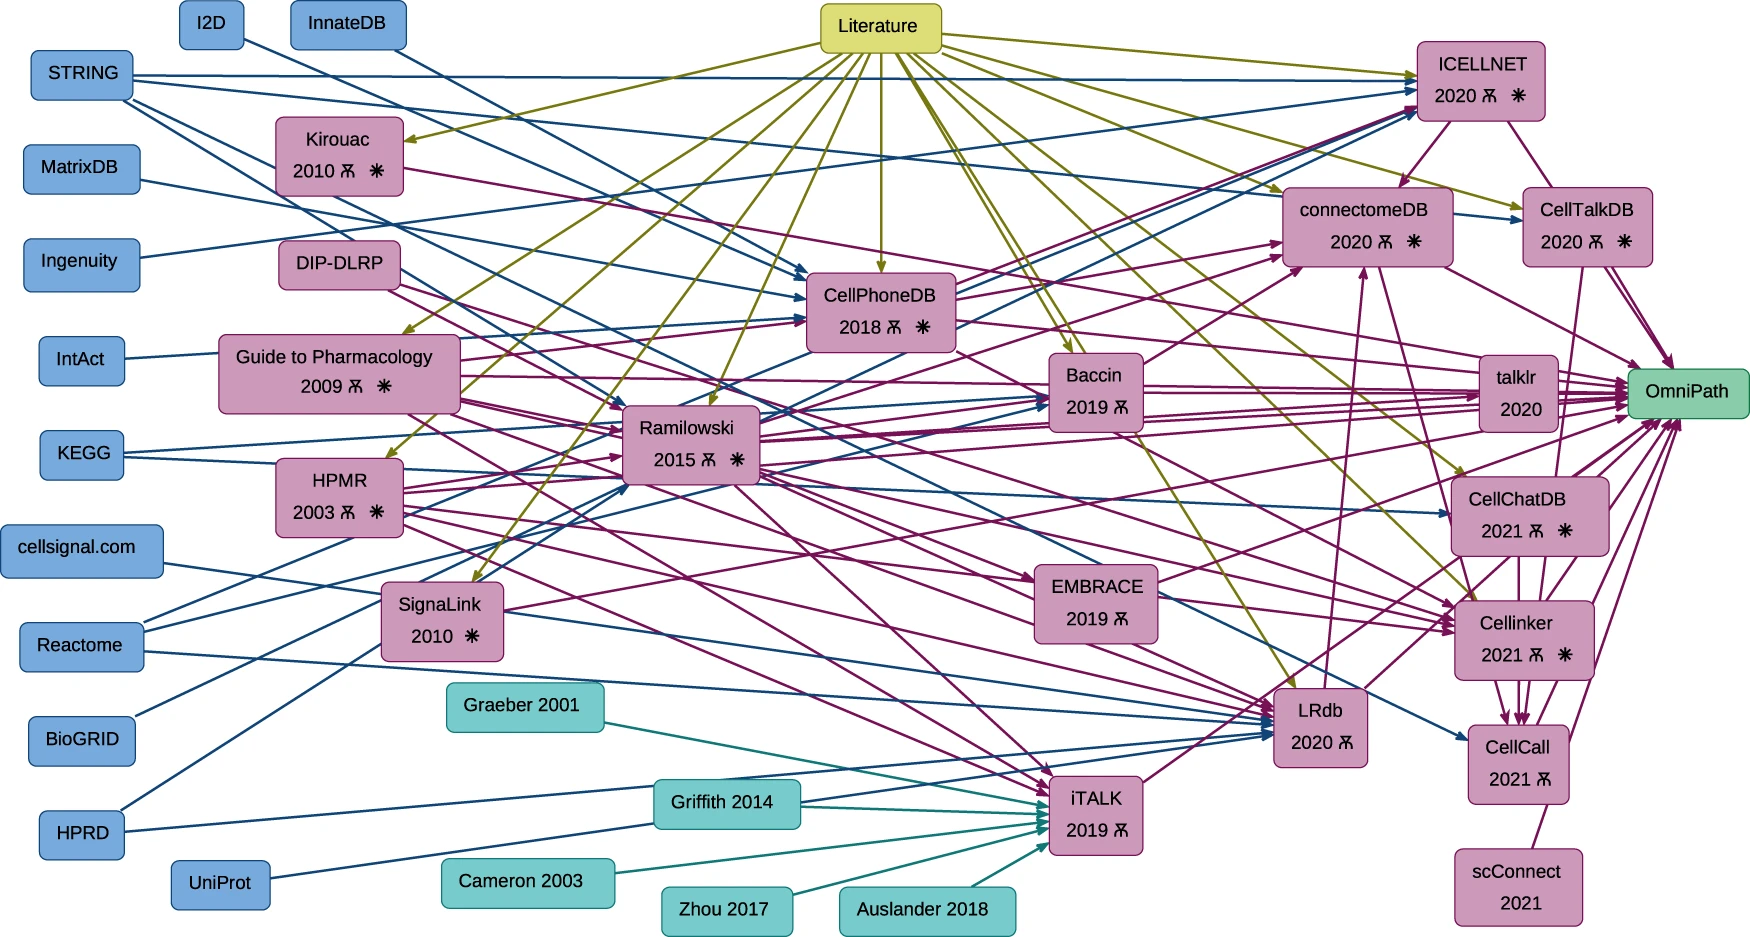
\includegraphics[width=0.85\linewidth,height=\textheight,keepaspectratio]{images/CCC_databases.png}

}

\caption{\label{fig-CCC-collection}The \textbf{lineages} of CCC
interaction database knowledge. \textcolor[HTML]{77aadc}{General
biological knowledge databases are reported in blue},
\textcolor[HTML]{cb9cbc}{CCC-dedicated resources in magenta}, and
\textcolor[HTML]{77cbcc}{additional resources included in \texttt{iTALK}
in cyan}, from \textcite{dimitrov2022nc}}

\end{figure}%

\global\setlength{\Oldarrayrulewidth}{\arrayrulewidth}

\global\setlength{\Oldtabcolsep}{\tabcolsep}

\setlength{\tabcolsep}{2pt}

\renewcommand*{\arraystretch}{1.5}



\providecommand{\ascline}[3]{\noalign{\global\arrayrulewidth #1}\arrayrulecolor[HTML]{#2}\cline{#3}}

\begin{longtable}[c]{cccccc}

\ascline{1.5pt}{666666}{1-6}

\multicolumn{1}{>{}l}{\textcolor[HTML]{000000}{\fontsize{11}{11}\selectfont{\global\setmainfont{Arial}{\textbf{Resource}}}}} & \multicolumn{1}{>{}l}{\textcolor[HTML]{000000}{\fontsize{11}{11}\selectfont{\global\setmainfont{Arial}{\textbf{Further\ curation}}}}} & \multicolumn{1}{>{}l}{\textcolor[HTML]{000000}{\fontsize{11}{11}\selectfont{\global\setmainfont{Arial}{\textbf{Sources}}}}} & \multicolumn{1}{>{}r}{\textcolor[HTML]{000000}{\fontsize{11}{11}\selectfont{\global\setmainfont{Arial}{\textbf{Interactions}}}}} & \multicolumn{1}{>{}r}{\textcolor[HTML]{000000}{\fontsize{11}{11}\selectfont{\global\setmainfont{Arial}{\textbf{Original\ curation}}}}} & \multicolumn{1}{>{}r}{\textcolor[HTML]{000000}{\fontsize{11}{11}\selectfont{\global\setmainfont{Arial}{\textbf{Overlap\ with\ curated\ set}}}}} \\

\ascline{1.5pt}{666666}{1-6}\endfirsthead 

\ascline{1.5pt}{666666}{1-6}

\multicolumn{1}{>{}l}{\textcolor[HTML]{000000}{\fontsize{11}{11}\selectfont{\global\setmainfont{Arial}{\textbf{Resource}}}}} & \multicolumn{1}{>{}l}{\textcolor[HTML]{000000}{\fontsize{11}{11}\selectfont{\global\setmainfont{Arial}{\textbf{Further\ curation}}}}} & \multicolumn{1}{>{}l}{\textcolor[HTML]{000000}{\fontsize{11}{11}\selectfont{\global\setmainfont{Arial}{\textbf{Sources}}}}} & \multicolumn{1}{>{}r}{\textcolor[HTML]{000000}{\fontsize{11}{11}\selectfont{\global\setmainfont{Arial}{\textbf{Interactions}}}}} & \multicolumn{1}{>{}r}{\textcolor[HTML]{000000}{\fontsize{11}{11}\selectfont{\global\setmainfont{Arial}{\textbf{Original\ curation}}}}} & \multicolumn{1}{>{}r}{\textcolor[HTML]{000000}{\fontsize{11}{11}\selectfont{\global\setmainfont{Arial}{\textbf{Overlap\ with\ curated\ set}}}}} \\

\ascline{1.5pt}{666666}{1-6}\endhead



\multicolumn{1}{>{}l}{\textcolor[HTML]{000000}{\fontsize{11}{11}\selectfont{\global\setmainfont{Arial}{Baccin2019/(a)27}}}} & \multicolumn{1}{>{}l}{\textcolor[HTML]{000000}{\fontsize{11}{11}\selectfont{\global\setmainfont{Arial}{Murine\ identifiers\ (only),\ Multimeric\ complexes}}}} & \multicolumn{1}{>{}l}{\textcolor[HTML]{000000}{\fontsize{11}{11}\selectfont{\global\setmainfont{Arial}{Ramilowski2015,\ KEGG\ REACTOME,\ Literature}}}} & \multicolumn{1}{>{}r}{\textcolor[HTML]{000000}{\fontsize{11}{11}\selectfont{\global\setmainfont{Arial}{1,625}}}} & \multicolumn{1}{>{}r}{\textcolor[HTML]{000000}{\fontsize{11}{11}\selectfont{\global\setmainfont{Arial}{TRUE}}}} & \multicolumn{1}{>{}r}{\textcolor[HTML]{000000}{\fontsize{11}{11}\selectfont{\global\setmainfont{Arial}{0.82}}}} \\





\multicolumn{1}{>{}l}{\textcolor[HTML]{000000}{\fontsize{11}{11}\selectfont{\global\setmainfont{Arial}{CellCall\ 22}}}} & \multicolumn{1}{>{}l}{\textcolor[HTML]{000000}{\fontsize{11}{11}\selectfont{\global\setmainfont{Arial}{Multimeric\ complexes,\ murine\ identifiers,\ Interactions\ downstream\ transcription\ factors\ (from\ KEGG),\ transcription\ factor\ regulons.}}}} & \multicolumn{1}{>{}l}{\textcolor[HTML]{000000}{\fontsize{11}{11}\selectfont{\global\setmainfont{Arial}{ConnectomeDB2020,\ CellLinker,\ CellTalkDB,\ CellChatDB,\ STRING}}}} & \multicolumn{1}{>{}r}{\textcolor[HTML]{000000}{\fontsize{11}{11}\selectfont{\global\setmainfont{Arial}{1,123}}}} & \multicolumn{1}{>{}r}{\textcolor[HTML]{000000}{\fontsize{11}{11}\selectfont{\global\setmainfont{Arial}{FALSE}}}} & \multicolumn{1}{>{}r}{\textcolor[HTML]{000000}{\fontsize{11}{11}\selectfont{\global\setmainfont{Arial}{0.51}}}} \\





\multicolumn{1}{>{}l}{\textcolor[HTML]{000000}{\fontsize{11}{11}\selectfont{\global\setmainfont{Arial}{CellChatDB13}}}} & \multicolumn{1}{>{}l}{\textcolor[HTML]{000000}{\fontsize{11}{11}\selectfont{\global\setmainfont{Arial}{Multimeric\ complexes,\ 229\ signaling\ pathway\ families,\ agonists\ and\ antagonists,\ co-receptors,\ localisations,\ Murine\ identifiers}}}} & \multicolumn{1}{>{}l}{\textcolor[HTML]{000000}{\fontsize{11}{11}\selectfont{\global\setmainfont{Arial}{KEGG,\ Literature}}}} & \multicolumn{1}{>{}r}{\textcolor[HTML]{000000}{\fontsize{11}{11}\selectfont{\global\setmainfont{Arial}{1,912}}}} & \multicolumn{1}{>{}r}{\textcolor[HTML]{000000}{\fontsize{11}{11}\selectfont{\global\setmainfont{Arial}{FALSE}}}} & \multicolumn{1}{>{}r}{\textcolor[HTML]{000000}{\fontsize{11}{11}\selectfont{\global\setmainfont{Arial}{0.84}}}} \\





\multicolumn{1}{>{}l}{\textcolor[HTML]{000000}{\fontsize{11}{11}\selectfont{\global\setmainfont{Arial}{Cellinker\ 15}}}} & \multicolumn{1}{>{}l}{\textcolor[HTML]{000000}{\fontsize{11}{11}\selectfont{\global\setmainfont{Arial}{Multimeric\ complexes,\ murine\ identifiers,\ sMOL\ ligands,\ intercellular\ communication\ roles}}}} & \multicolumn{1}{>{}l}{\textcolor[HTML]{000000}{\fontsize{11}{11}\selectfont{\global\setmainfont{Arial}{DLRP,\ HPMR,\ CellPhoneDB,\ Guide2Pharma,\ Literature}}}} & \multicolumn{1}{>{}r}{\textcolor[HTML]{000000}{\fontsize{11}{11}\selectfont{\global\setmainfont{Arial}{3,701}}}} & \multicolumn{1}{>{}r}{\textcolor[HTML]{000000}{\fontsize{11}{11}\selectfont{\global\setmainfont{Arial}{FALSE}}}} & \multicolumn{1}{>{}r}{\textcolor[HTML]{000000}{\fontsize{11}{11}\selectfont{\global\setmainfont{Arial}{0.71}}}} \\





\multicolumn{1}{>{}l}{\textcolor[HTML]{000000}{\fontsize{11}{11}\selectfont{\global\setmainfont{Arial}{CellPhoneDB\ 7,79,80}}}} & \multicolumn{1}{>{}l}{\textcolor[HTML]{000000}{\fontsize{11}{11}\selectfont{\global\setmainfont{Arial}{Multimeric\ complexes,\ intercellular\ communication\ roles}}}} & \multicolumn{1}{>{}l}{\textcolor[HTML]{000000}{\fontsize{11}{11}\selectfont{\global\setmainfont{Arial}{Guide2Pharma,\ I2D,\ IntAct,\ UniProt,\ Literature,\ HPIDB}}}} & \multicolumn{1}{>{}r}{\textcolor[HTML]{000000}{\fontsize{11}{11}\selectfont{\global\setmainfont{Arial}{1,219}}}} & \multicolumn{1}{>{}r}{\textcolor[HTML]{000000}{\fontsize{11}{11}\selectfont{\global\setmainfont{Arial}{FALSE}}}} & \multicolumn{1}{>{}r}{\textcolor[HTML]{000000}{\fontsize{11}{11}\selectfont{\global\setmainfont{Arial}{0.90}}}} \\





\multicolumn{1}{>{}l}{\textcolor[HTML]{000000}{\fontsize{11}{11}\selectfont{\global\setmainfont{Arial}{CellTalkDB25}}}} & \multicolumn{1}{>{}l}{\textcolor[HTML]{000000}{\fontsize{11}{11}\selectfont{\global\setmainfont{Arial}{Murine\ identifiers}}}} & \multicolumn{1}{>{}l}{\textcolor[HTML]{000000}{\fontsize{11}{11}\selectfont{\global\setmainfont{Arial}{STRING,\ Literature}}}} & \multicolumn{1}{>{}r}{\textcolor[HTML]{000000}{\fontsize{11}{11}\selectfont{\global\setmainfont{Arial}{3,392}}}} & \multicolumn{1}{>{}r}{\textcolor[HTML]{000000}{\fontsize{11}{11}\selectfont{\global\setmainfont{Arial}{FALSE}}}} & \multicolumn{1}{>{}r}{\textcolor[HTML]{000000}{\fontsize{11}{11}\selectfont{\global\setmainfont{Arial}{1.00}}}} \\





\multicolumn{1}{>{}l}{\textcolor[HTML]{000000}{\fontsize{11}{11}\selectfont{\global\setmainfont{Arial}{ConnectomeDB202010}}}} & \multicolumn{1}{>{}l}{\textcolor[HTML]{000000}{\fontsize{11}{11}\selectfont{\global\setmainfont{Arial}{Intercellular\ communication\ roles}}}} & \multicolumn{1}{>{}l}{\textcolor[HTML]{000000}{\fontsize{11}{11}\selectfont{\global\setmainfont{Arial}{Ramilowski2015,\ CellphoneDB,\ Baccin2019,\ LRdb,\ ICELLNET,\ Literature}}}} & \multicolumn{1}{>{}r}{\textcolor[HTML]{000000}{\fontsize{11}{11}\selectfont{\global\setmainfont{Arial}{2,266}}}} & \multicolumn{1}{>{}r}{\textcolor[HTML]{000000}{\fontsize{11}{11}\selectfont{\global\setmainfont{Arial}{FALSE}}}} & \multicolumn{1}{>{}r}{\textcolor[HTML]{000000}{\fontsize{11}{11}\selectfont{\global\setmainfont{Arial}{0.99}}}} \\





\multicolumn{1}{>{}l}{\textcolor[HTML]{000000}{\fontsize{11}{11}\selectfont{\global\setmainfont{Arial}{EMBRACE(a)54}}}} & \multicolumn{1}{>{}l}{\textcolor[HTML]{000000}{\fontsize{11}{11}\selectfont{\global\setmainfont{Arial}{Murine\ identifiers}}}} & \multicolumn{1}{>{}l}{\textcolor[HTML]{000000}{\fontsize{11}{11}\selectfont{\global\setmainfont{Arial}{Ramilowski2015}}}} & \multicolumn{1}{>{}r}{\textcolor[HTML]{000000}{\fontsize{11}{11}\selectfont{\global\setmainfont{Arial}{1,639}}}} & \multicolumn{1}{>{}r}{\textcolor[HTML]{000000}{\fontsize{11}{11}\selectfont{\global\setmainfont{Arial}{FALSE}}}} & \multicolumn{1}{>{}r}{\textcolor[HTML]{000000}{\fontsize{11}{11}\selectfont{\global\setmainfont{Arial}{0.97}}}} \\





\multicolumn{1}{>{}l}{\textcolor[HTML]{000000}{\fontsize{11}{11}\selectfont{\global\setmainfont{Arial}{Guide2Pharma(b)32}}}} & \multicolumn{1}{>{}l}{\textcolor[HTML]{000000}{\fontsize{11}{11}\selectfont{\global\setmainfont{Arial}{-}}}} & \multicolumn{1}{>{}l}{\textcolor[HTML]{000000}{\fontsize{11}{11}\selectfont{\global\setmainfont{Arial}{Literature}}}} & \multicolumn{1}{>{}r}{\textcolor[HTML]{000000}{\fontsize{11}{11}\selectfont{\global\setmainfont{Arial}{665}}}} & \multicolumn{1}{>{}r}{\textcolor[HTML]{000000}{\fontsize{11}{11}\selectfont{\global\setmainfont{Arial}{FALSE}}}} & \multicolumn{1}{>{}r}{\textcolor[HTML]{000000}{\fontsize{11}{11}\selectfont{\global\setmainfont{Arial}{1.00}}}} \\





\multicolumn{1}{>{}l}{\textcolor[HTML]{000000}{\fontsize{11}{11}\selectfont{\global\setmainfont{Arial}{HPMR33}}}} & \multicolumn{1}{>{}l}{\textcolor[HTML]{000000}{\fontsize{11}{11}\selectfont{\global\setmainfont{Arial}{-}}}} & \multicolumn{1}{>{}l}{\textcolor[HTML]{000000}{\fontsize{11}{11}\selectfont{\global\setmainfont{Arial}{Literature}}}} & \multicolumn{1}{>{}r}{\textcolor[HTML]{000000}{\fontsize{11}{11}\selectfont{\global\setmainfont{Arial}{596}}}} & \multicolumn{1}{>{}r}{\textcolor[HTML]{000000}{\fontsize{11}{11}\selectfont{\global\setmainfont{Arial}{FALSE}}}} & \multicolumn{1}{>{}r}{\textcolor[HTML]{000000}{\fontsize{11}{11}\selectfont{\global\setmainfont{Arial}{1.00}}}} \\





\multicolumn{1}{>{}l}{\textcolor[HTML]{000000}{\fontsize{11}{11}\selectfont{\global\setmainfont{Arial}{ICELLNET26}}}} & \multicolumn{1}{>{}l}{\textcolor[HTML]{000000}{\fontsize{11}{11}\selectfont{\global\setmainfont{Arial}{Multimeric\ complexes,
}}}\textcolor[HTML]{000000}{\fontsize{11}{11}\selectfont{\global\setmainfont{Arial}{\linebreak }}}\textcolor[HTML]{000000}{\fontsize{11}{11}\selectfont{\global\setmainfont{Arial}{Signalling\ families,
}}}\textcolor[HTML]{000000}{\fontsize{11}{11}\selectfont{\global\setmainfont{Arial}{\linebreak }}}\textcolor[HTML]{000000}{\fontsize{11}{11}\selectfont{\global\setmainfont{Arial}{Cytokine-focus}}}} & \multicolumn{1}{>{}l}{\textcolor[HTML]{000000}{\fontsize{11}{11}\selectfont{\global\setmainfont{Arial}{STRING,\ Ingenuity,\ BioGRID,\ Reactome,\ CellPhoneDB}}}} & \multicolumn{1}{>{}r}{\textcolor[HTML]{000000}{\fontsize{11}{11}\selectfont{\global\setmainfont{Arial}{738}}}} & \multicolumn{1}{>{}r}{\textcolor[HTML]{000000}{\fontsize{11}{11}\selectfont{\global\setmainfont{Arial}{FALSE}}}} & \multicolumn{1}{>{}r}{\textcolor[HTML]{000000}{\fontsize{11}{11}\selectfont{\global\setmainfont{Arial}{0.95}}}} \\





\multicolumn{1}{>{}l}{\textcolor[HTML]{000000}{\fontsize{11}{11}\selectfont{\global\setmainfont{Arial}{iTALK5}}}} & \multicolumn{1}{>{}l}{\textcolor[HTML]{000000}{\fontsize{11}{11}\selectfont{\global\setmainfont{Arial}{Ligand\ categories}}}} & \multicolumn{1}{>{}l}{\textcolor[HTML]{000000}{\fontsize{11}{11}\selectfont{\global\setmainfont{Arial}{Ramilowski2015,\ HPMR,
}}}\textcolor[HTML]{000000}{\fontsize{11}{11}\selectfont{\global\setmainfont{Arial}{\linebreak }}}\textcolor[HTML]{000000}{\fontsize{11}{11}\selectfont{\global\setmainfont{Arial}{Guide2Pharma,\ Graeber2001,\ Griffith2014,\ Cameron2003,\ Zhou2017,\ Auslander2018}}}} & \multicolumn{1}{>{}r}{\textcolor[HTML]{000000}{\fontsize{11}{11}\selectfont{\global\setmainfont{Arial}{2,566}}}} & \multicolumn{1}{>{}r}{\textcolor[HTML]{000000}{\fontsize{11}{11}\selectfont{\global\setmainfont{Arial}{TRUE}}}} & \multicolumn{1}{>{}r}{\textcolor[HTML]{000000}{\fontsize{11}{11}\selectfont{\global\setmainfont{Arial}{0.96}}}} \\





\multicolumn{1}{>{}l}{\textcolor[HTML]{000000}{\fontsize{11}{11}\selectfont{\global\setmainfont{Arial}{Kirouac201038}}}} & \multicolumn{1}{>{}l}{\textcolor[HTML]{000000}{\fontsize{11}{11}\selectfont{\global\setmainfont{Arial}{-}}}} & \multicolumn{1}{>{}l}{\textcolor[HTML]{000000}{\fontsize{11}{11}\selectfont{\global\setmainfont{Arial}{Literature,\ COPE}}}} & \multicolumn{1}{>{}r}{\textcolor[HTML]{000000}{\fontsize{11}{11}\selectfont{\global\setmainfont{Arial}{152}}}} & \multicolumn{1}{>{}r}{\textcolor[HTML]{000000}{\fontsize{11}{11}\selectfont{\global\setmainfont{Arial}{FALSE}}}} & \multicolumn{1}{>{}r}{\textcolor[HTML]{000000}{\fontsize{11}{11}\selectfont{\global\setmainfont{Arial}{1.00}}}} \\





\multicolumn{1}{>{}l}{\textcolor[HTML]{000000}{\fontsize{11}{11}\selectfont{\global\setmainfont{Arial}{LRdb11}}}} & \multicolumn{1}{>{}l}{\textcolor[HTML]{000000}{\fontsize{11}{11}\selectfont{\global\setmainfont{Arial}{-}}}} & \multicolumn{1}{>{}l}{\textcolor[HTML]{000000}{\fontsize{11}{11}\selectfont{\global\setmainfont{Arial}{cellsignal.com,\ Ramilowski2015,\ Guide2Pharma,\ HPMR,\ HPRD,\ Reactome,\ UniProt,\ Literature}}}} & \multicolumn{1}{>{}r}{\textcolor[HTML]{000000}{\fontsize{11}{11}\selectfont{\global\setmainfont{Arial}{3,228}}}} & \multicolumn{1}{>{}r}{\textcolor[HTML]{000000}{\fontsize{11}{11}\selectfont{\global\setmainfont{Arial}{TRUE}}}} & \multicolumn{1}{>{}r}{\textcolor[HTML]{000000}{\fontsize{11}{11}\selectfont{\global\setmainfont{Arial}{0.96}}}} \\





\multicolumn{1}{>{}l}{\textcolor[HTML]{000000}{\fontsize{11}{11}\selectfont{\global\setmainfont{Arial}{Ramilowski201534}}}} & \multicolumn{1}{>{}l}{\textcolor[HTML]{000000}{\fontsize{11}{11}\selectfont{\global\setmainfont{Arial}{-}}}} & \multicolumn{1}{>{}l}{\textcolor[HTML]{000000}{\fontsize{11}{11}\selectfont{\global\setmainfont{Arial}{DLRP,\ HPMR,\ IUPHAR,\ HPRD,\ STRING,\ Literature}}}} & \multicolumn{1}{>{}r}{\textcolor[HTML]{000000}{\fontsize{11}{11}\selectfont{\global\setmainfont{Arial}{1,889}}}} & \multicolumn{1}{>{}r}{\textcolor[HTML]{000000}{\fontsize{11}{11}\selectfont{\global\setmainfont{Arial}{FALSE}}}} & \multicolumn{1}{>{}r}{\textcolor[HTML]{000000}{\fontsize{11}{11}\selectfont{\global\setmainfont{Arial}{0.99}}}} \\





\multicolumn{1}{>{}l}{\textcolor[HTML]{000000}{\fontsize{11}{11}\selectfont{\global\setmainfont{Arial}{scConnect}}}} & \multicolumn{1}{>{}l}{\textcolor[HTML]{000000}{\fontsize{11}{11}\selectfont{\global\setmainfont{Arial}{-}}}} & \multicolumn{1}{>{}l}{\textcolor[HTML]{000000}{\fontsize{11}{11}\selectfont{\global\setmainfont{Arial}{Guide2Pharma}}}} & \multicolumn{1}{>{}r}{\textcolor[HTML]{000000}{\fontsize{11}{11}\selectfont{\global\setmainfont{Arial}{479}}}} & \multicolumn{1}{>{}r}{\textcolor[HTML]{000000}{\fontsize{11}{11}\selectfont{\global\setmainfont{Arial}{FALSE}}}} & \multicolumn{1}{>{}r}{\textcolor[HTML]{000000}{\fontsize{11}{11}\selectfont{\global\setmainfont{Arial}{0.92}}}} \\

\ascline{1.5pt}{666666}{1-6}



\caption{\label{tbl-PKN-LR}Available prior knowledge resources tested in
benchmark \textcite{dimitrov2022nc} are largely composed of
\textbf{ligand-receptor}, extracellular matrix, and \textbf{adhesion
interactions}. Note that most of these resources, notably the curated
ones, have been collectively collected in the
\href{https://r.omnipathdb.org}{\texttt{OmniPathR} database}, from
\textcite{turei2021msb}.}

\tabularnewline
\end{longtable}

\arrayrulecolor[HTML]{000000}

\global\setlength{\arrayrulewidth}{\Oldarrayrulewidth}

\global\setlength{\tabcolsep}{\Oldtabcolsep}

\renewcommand*{\arraystretch}{1}

\subsection{Hurdles for benchmarking cell-cell communication inference
methods}\label{sec-hurdles-benchmark}

\subsubsection{Partial overlap between CCC
databases}\label{partial-overlap-between-ccc-databases}

\subsubsection{Metric quantifying spatial gene expression
distribution.}\label{metric-quantifying-spatial-gene-expression-distribution.}

\begin{itemize}
\tightlist
\item
  \textbf{Wasserstein distributions} to compare probability
  distributions:

  \begin{itemize}
  \tightlist
  \item
    Represents the minimum total transport cost between two
    distributions.
  \item
    Use of Regularised versions, such as the \textbf{Sinkhorn
    algorithm}, for faster computation and reduces influence of extreme
    observations.
  \item
    Detailled theoretical explanations:
    \autocite{rolet2016p1icais,huizing2022,solomon2017smmo,peyre}.
  \item
    \textbf{Consider truly spatial distributions and statistics}
    -\textgreater{} the \textbf{Fused Gromov-Wasserstein (FGW) distance}
    is a generalization of the Gromov-Wasserstein (GW) distance that
    accounts for both \textbf{feature} (pointwise) and
    \textbf{structural similarities} (geometric) between two metric
    measure spaces. Enables to maintain the \textbf{graph structure}, as
    suggested in {[}\textcite{vayer2020a};titouan2019p3icml{]}.
  \end{itemize}
\end{itemize}

\subsubsection{Annotate cell-populations in spatial
omics}\label{annotate-cell-populations-in-spatial-omics}

Recent deconvolution papers include:

\begin{itemize}
\tightlist
\item
  STRIDE
\end{itemize}

Relevant benchmark papers include:

\begin{itemize}
\tightlist
\item
  \href{https://www.nature.com/articles/s41592-024-02325-3}{Systematic
  comparison of sequencing-based spatial transcriptomic methods}, from
  \textcite{you2024nm}.
\item
  \href{https://www.nature.com/articles/s41467-023-37168-7}{A
  comprehensive benchmarking with practical guidelines for cellular
  deconvolution of spatial transcriptomics}, from \textcite{li2023nc}.
\item
  \href{https://www.nature.com/articles/s41592-022-01480-9}{Benchmarking
  spatial and single-cell transcriptomics integration methods for
  transcript distribution prediction and cell type deconvolution}, from
  \textcite{li2022nm}. Conclusions from the paper are reported in
  Important~\ref{imp-spatial-benchmark-deconvolution}.
\end{itemize}

\begin{tcolorbox}[enhanced jigsaw, coltitle=black, colbacktitle=quarto-callout-important-color!10!white, toptitle=1mm, breakable, bottomrule=.15mm, opacityback=0, title=\textcolor{quarto-callout-important-color}{\faExclamation}\hspace{0.5em}{Important \ref*{imp-spatial-benchmark-deconvolution}: Best spatial deconvolution algorithms}, opacitybacktitle=0.6, arc=.35mm, leftrule=.75mm, titlerule=0mm, bottomtitle=1mm, rightrule=.15mm, toprule=.15mm, left=2mm, colframe=quarto-callout-important-color-frame, colback=white]

\quartocalloutimp{imp-spatial-benchmark-deconvolution} 

From \textcite{li2022nm}, Tangram, gimVI, and SpaGE outperformed other
integration methods for predicting the spatial distribution of RNA
transcripts, whereas Cell2location, SpatialDWLS, and RCTD are the
top-performing methods for the cell type deconvolution of spots.

\end{tcolorbox}

\begin{figure}[H]

{\centering \pandocbounded{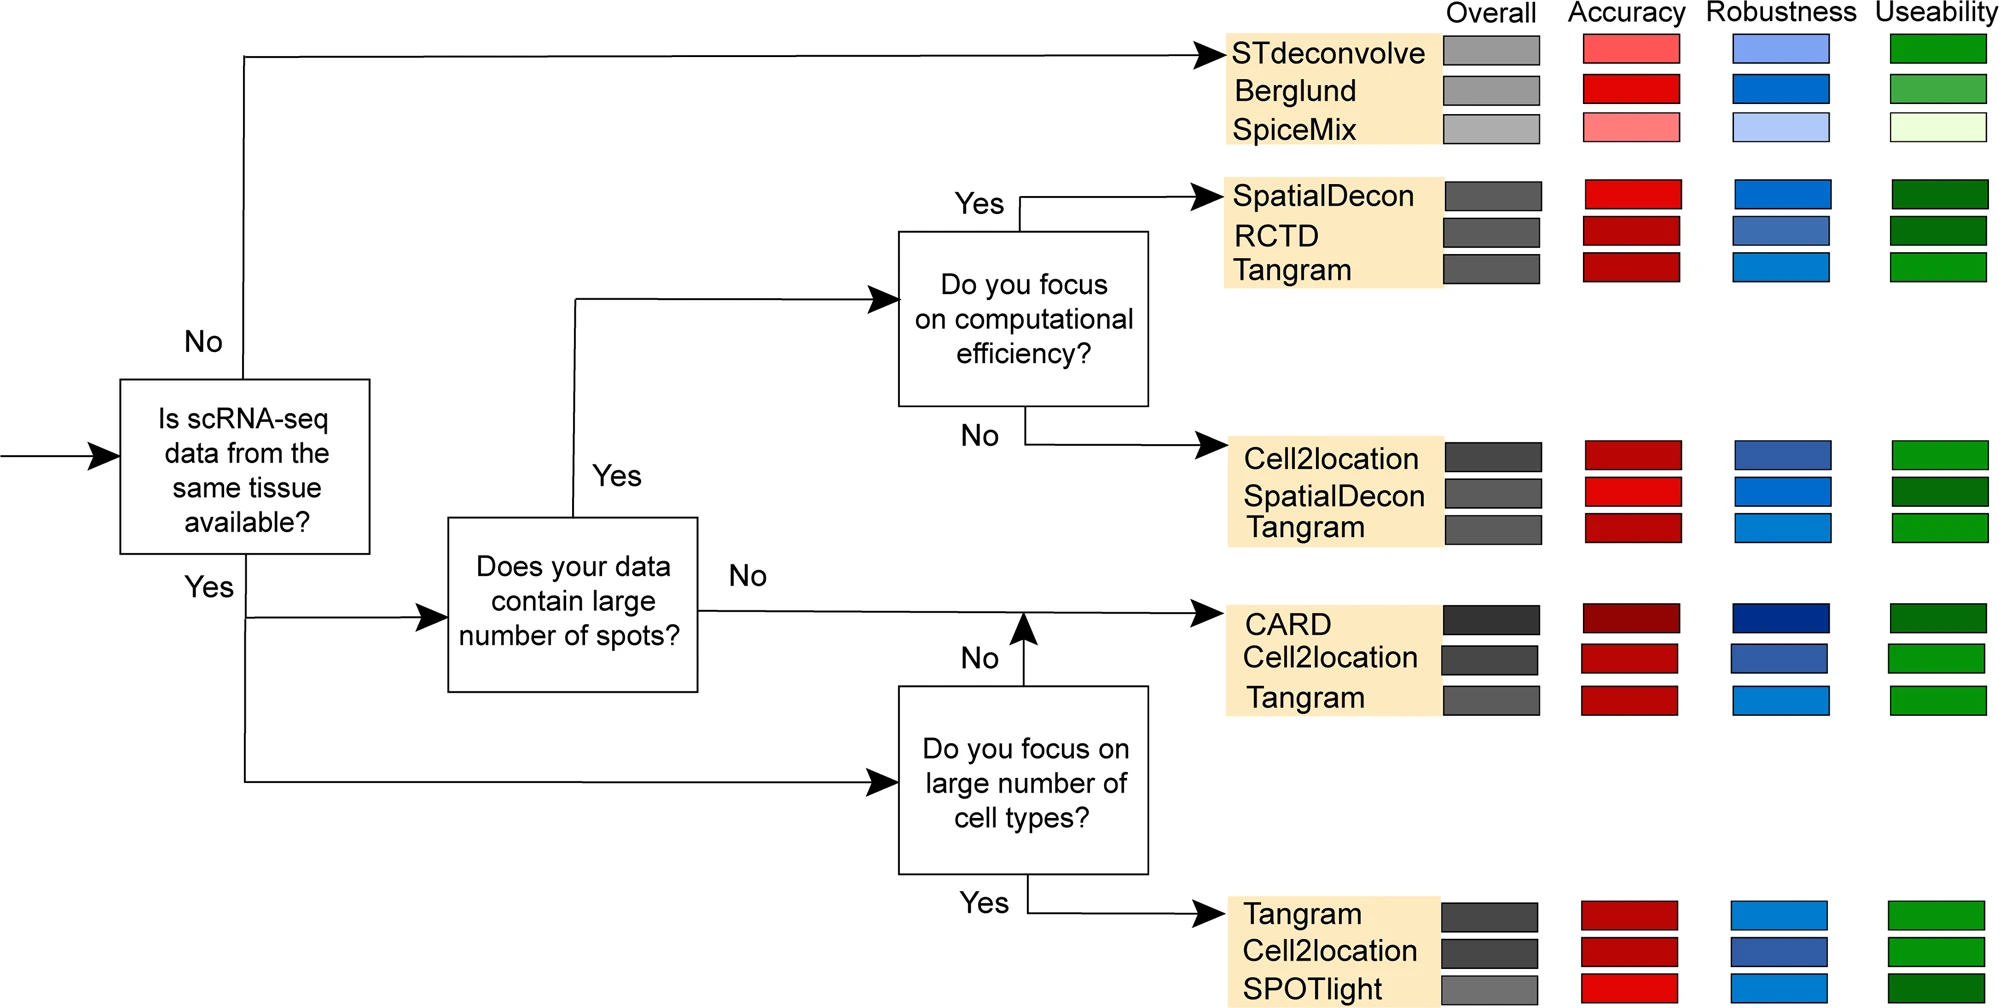
\includegraphics[keepaspectratio]{images/benchmark_deconvolution.png}}

}

\caption{Benchmark decision tree for Deconvolution Algorithms applied to
Spatial Transcriptomics}

\end{figure}%

\paragraph{Dynamic integration and mapping of cell
populations}\label{dynamic-integration-and-mapping-of-cell-populations}

\begin{itemize}
\item
  \href{https://www.nature.com/articles/s41467-025-56523-4}{\texttt{SIMO},
  for Spatial Integration of Multi-Omics}, from \textcite{yang2025nc}.

  \begin{itemize}
  \tightlist
  \item
    Probabilistic alignment relying on the fused
    \textbf{Gromov-Wasserstein optimal transport} algorithm
  \item
    Integrates multiple single-cell modalities, such as chromatin
    accessibility and DNA methylation.
  \item
    Integrates co-localisation spatial patterns.
  \end{itemize}
\end{itemize}

\begin{tcolorbox}[enhanced jigsaw, coltitle=black, colbacktitle=quarto-callout-caution-color!10!white, toptitle=1mm, breakable, bottomrule=.15mm, opacityback=0, title=\textcolor{quarto-callout-caution-color}{\faFire}\hspace{0.5em}{Major hurdles when performing cell type annotation with a dynamic
dimension}, opacitybacktitle=0.6, arc=.35mm, leftrule=.75mm, titlerule=0mm, bottomtitle=1mm, rightrule=.15mm, toprule=.15mm, left=2mm, colframe=quarto-callout-caution-color-frame, colback=white]

Major challenge is to track invidual cells's fate across time points,
with both \textbf{experimental variability} (distinct technologies and
experimental conditions across time points, image rotation and
distortion, etc.) and \textbf{biological variability} (mutations in
tumoral environment, cell differentiation in early-developmental stages,
cell deaths, \ldots).

\end{tcolorbox}

\subsubsection{Discriminate paracrine or juxtacrine with endocrine
signalling (short vs long-range
communications)}\label{discriminate-paracrine-or-juxtacrine-with-endocrine-signalling-short-vs-long-range-communications}

\begin{enumerate}
\def\labelenumi{\arabic{enumi}.}
\tightlist
\item
  Discriminate between short- and long-range cell-cell communications:
\end{enumerate}

\begin{itemize}
\tightlist
\item
  Current Use of \(k\)-means, to be replaced with:

  \begin{itemize}
  \tightlist
  \item
    Use of mixture models to characterise and automatically retrive the
    threshold
  \item
    \href{https://www.linkedin.com/posts/vlevorato_machinelearning-datascience-unsupervised-activity-7289567831145279490-Ibchs}{\texttt{BanditPAM}}
  \item
    \href{https://www.linkedin.com/posts/vlevorato_datascience-machinelearning-unsupervised-activity-7292093235366121472-jMMg}{Selection
    of the number of clusters}
  \item
    Even better, review latest spatial methods tailored to spatial
    clustering.
  \end{itemize}
\end{itemize}

\begin{enumerate}
\def\labelenumi{\arabic{enumi}.}
\setcounter{enumi}{1}
\tightlist
\item
  Compare distances by:
\end{enumerate}

\begin{enumerate}
\def\labelenumi{\roman{enumi}.}
\tightlist
\item
  Use of \textbf{Distance Enrichment Score} (compare the distribution of
  predicted short-rank and long-rank interactions with what's observed),
  similar to GSEA as showcased in \autocite{subramanian2005pnas}, and
  theretically largely inspired from the \textbf{Kolmogorov-Smirnov}
  statistical test. -
  \href{https://www.linkedin.com/posts/adrianolszewski_statistics-datascience-activity-7256312446737387520-J8zk}{General
  advises for enhanced comparision of statistical distributions}.
  Indeed, the KS only evaluates the maximal discrepancy between two
  distributions, and not the whole statistical distribution.\\
\item
  Confusion matrix between predicted \textbf{short-range} and
  \textbf{long-range} communications, benchmarked against the consensual
  setting.
\end{enumerate}

\subsubsection{Simulate in-silico spatial transcriptomic
distributions}\label{simulate-in-silico-spatial-transcriptomic-distributions}

\paragraph{Single-cell simulations}\label{single-cell-simulations}

\begin{itemize}
\tightlist
\item
  \href{https://genomebiology.biomedcentral.com/articles/10.1186/s13059-017-1305-0}{\texttt{Splatter}},
  from \textcite{zappia2017gb}.

  \begin{itemize}
  \tightlist
  \item
    A two-stage simulation process: 1.Estimation of the parameters from
    realistic datasets.

    \begin{enumerate}
    \def\labelenumi{\arabic{enumi}.}
    \setcounter{enumi}{1}
    \tightlist
    \item
      Generation of a synthetic dataset from the prior parameters
      inferred in stage 1.
    \end{enumerate}
  \item
    Avalaible as a
    \href{https://www.bioconductor.org/packages/release/bioc/html/splatter.html}{Bioconductor
    R package}.
  \item
    Six simulation scenarios:

    \begin{enumerate}
    \def\labelenumi{\arabic{enumi}.}
    \tightlist
    \item
      \textbf{``Simple''}: Negative binomial distributions.
    \item
      Extension to model 1 by adding technical noise resulting from
      distinct depth sequencing (aka library size factor).
    \item
      Adds an additional \textbf{batch effect} to model 2.
    \item
      Mixtures of potential distinct probability distributions.
    \item
      BASiCS: models both biological and technical variation evaluated
      through \textbf{spike-ins} genes
    \item
      Splat: Gamma (for mean gene expression)-Poisson (for cells counts)
      hierarchical model + inclusion of outliers + inclusion of
      \textbf{drop-outs} + library size + \textbf{Biological Coefficient
      of Variation} to enforce a \emph{mean-variance} trend.
    \item
      \href{https://static-content.springer.com/esm/art\%3A10.1186\%2Fs13059-017-1305-0/MediaObjects/13059_2017_1305_MOESM1_ESM.pdf}{DAGs
      of the hierarchical models used for simulation}.
    \end{enumerate}
  \item
    Tailored for modelling scRNASeq datasets only, no accounting for
    spatial dispersion.
  \end{itemize}
\item
  \href{https://github.com/JSB-UCLA/scDesign2}{\texttt{scDesign2}}:

  \begin{itemize}
  \tightlist
  \item
    Tailored towards single-cell modelling and simulations only.
  \item
    Uses \textbf{copulas}, only modelling the marginal distirbution of
    gene expression. Report to Tip~\ref{tip-copula} for details.
  \item
    Only avalaible as the Github R repository
    \href{https://github.com/JSB-UCLA/scDesign2}{\texttt{scDesign2}}
    with following
    \href{https://htmlpreview.github.io/?https://github.com/JSB-UCLA/scDesign2/blob/master/vignettes/scDesign2.html.}{tutorial}
  \end{itemize}
\end{itemize}

\begin{tcolorbox}[enhanced jigsaw, coltitle=black, colbacktitle=quarto-callout-tip-color!10!white, toptitle=1mm, breakable, bottomrule=.15mm, opacityback=0, title=\textcolor{quarto-callout-tip-color}{\faLightbulb}\hspace{0.5em}{Tip \ref*{tip-copula}: Copula Decomposition of Multivariate Distributions: the Sklar's Theorem}, opacitybacktitle=0.6, arc=.35mm, leftrule=.75mm, titlerule=0mm, bottomtitle=1mm, rightrule=.15mm, toprule=.15mm, left=2mm, colframe=quarto-callout-tip-color-frame, colback=white]

\quartocallouttip{tip-copula} 

Considering a multivariate probability distribution, characterised by
\textbf{random vector} \(\mathbf{X} = (X_1, X_2, ..., X_d)\) if
dimension \(d\), the Sklar's theorem, aka the \textbf{copula
decomposition}, allows decomposing the \textbf{joint cumulative
distribution function (CDF)} into their \textbf{marginals} (no
correlation between them by definition) and a function that describes
the \textbf{dependence structure} (aka the covariance structure) between
them. The \emph{copula} is this coupling function, hence the name.

In details, for a \textbf{d-dimensional} random vector
\(\mathbf{X} = (X_1, ..., X_d)\) with joint CDF \(F(x_1, ..., x_d)\) and
continuous marginal CDFs \(F_1(x_1), \ldots, F_d(x_d)\), there exists a
unique \textbf{copula function} \(C\) that allows decomposition of the
\textbf{joint probability density function (PDF)} of \(\mathbf{X}\) into
(see (Equation~\ref{eq-sklar-theorem})):

\begin{equation}\phantomsection\label{eq-sklar-theorem}{
f(x_1, ..., x_d) = \overbrace{c(F_1(x_1), ..., F_d(x_d))}^{\text{Copula characterising covariance structure}} \overbrace{\prod_{i=1}^{d} f_i(x_i)}^{\text{Marginal density functions}}
}\end{equation}

\textbf{If the marginal distributions are continuous, this decomposition
is unique.}

\end{tcolorbox}

\paragraph{Spatial simulations}\label{spatial-simulations}

\begin{itemize}
\tightlist
\item
  \href{https://github.com/Teichlab/SpatialDE}{\texttt{SpatialDE}}, from
  \autocite{svensson2018nm}:

  \begin{itemize}
  \tightlist
  \item
    Models interactions across gene expression profiles considering a
    multivariate Gaussian distribution, whose covariance term captures
    both \textbf{spatial covariance} and \textbf{non spatial variance}
    (assumption of IID noise).
  \item
    Inspired from GP (Gaussian-Process) models, here tailored to spatial
    transcriptomic data.
  \item
    Not really tailored for simulating different kinds of spatial
    transcriptomc expression, model quite specific.
  \item
    Implemented in Python.
  \end{itemize}
\item
  \href{https://www.nature.com/articles/s41467-023-37822-0}{\texttt{spasim}},
  from \textcite{feng2023nc}.

  \begin{itemize}
  \tightlist
  \item
    Tailored for simulating \textbf{spatial imaging} rather than spatial
    omics distribution.
  \item
    Relevant enumeration of \textbf{cell colocalisation} spatial metrics
    in {[}https://www.nature.com/articles/s41467-023-37822-0\#Sec10{]}:

    \begin{itemize}
    \tightlist
    \item
      Average pairwise distance (APD)
    \item
      Average minimum distance (AMD)
    \item
      Cells in neighborhood (CIN)
    \item
      Mixing score (MS) and Normalized mixing score (NMS)
    \item
      Area under the curve of the cross K function (AUC)
    \item
      Cross K intersection (CKI)
    \item
      Localized entropy, Saptial heterogeneity and entropy gradient.
    \item
      Average nearest neighbor index (ANNI) to detect clusters of cell.
    \item
      Implemented as a
      \href{https://bioconductor.org/packages/spaSim/}{BioConductor
      package} apired with
      \href{https://trigosteam.github.io/spaSim/}{spaSim tutorial}.
    \end{itemize}
  \end{itemize}
\item
  \href{https://github.com/ZhangLabGT/scMultiSim}{\texttt{scMultiSim}},
  from \textcite{li2023rs}:

  \begin{itemize}
  \item
    Certainly, the most comprehensive simulation framework so far.
    Includes modelling of:

    \begin{itemize}
    \tightlist
    \item
      Dynamic variations (changes of GRNs across time points, aka RNA
      velocity + varying proportions of spliced and unspliced gene
      expression, in relation with chromatin accessibility quantified by
      scATACseq + cell line tree lineage).
    \item
      Multi-modal (gene expression, chromatin accessibility)
    \item
      Accounts for technical variations (library preparation noise
      including sequencing depth and cell-specific transcript capture +
      batch effet), inspired from \texttt{SymSim} \autocite{zhang2019nc}
      scRNASeq simulator.
    \end{itemize}
  \item
    A
    \href{https://www.bioconductor.org/packages/release/bioc/html/scMultiSim.html}{BioConductor
    package}, with its
    \href{https://zhanglabgt.github.io/scMultiSim/articles/spatialCCI.html}{spatial
    transcriptomics tutorial}. See Figure~\ref{fig-scMultisim} below for
    details.
  \end{itemize}
\end{itemize}

\begin{figure}

\centering{

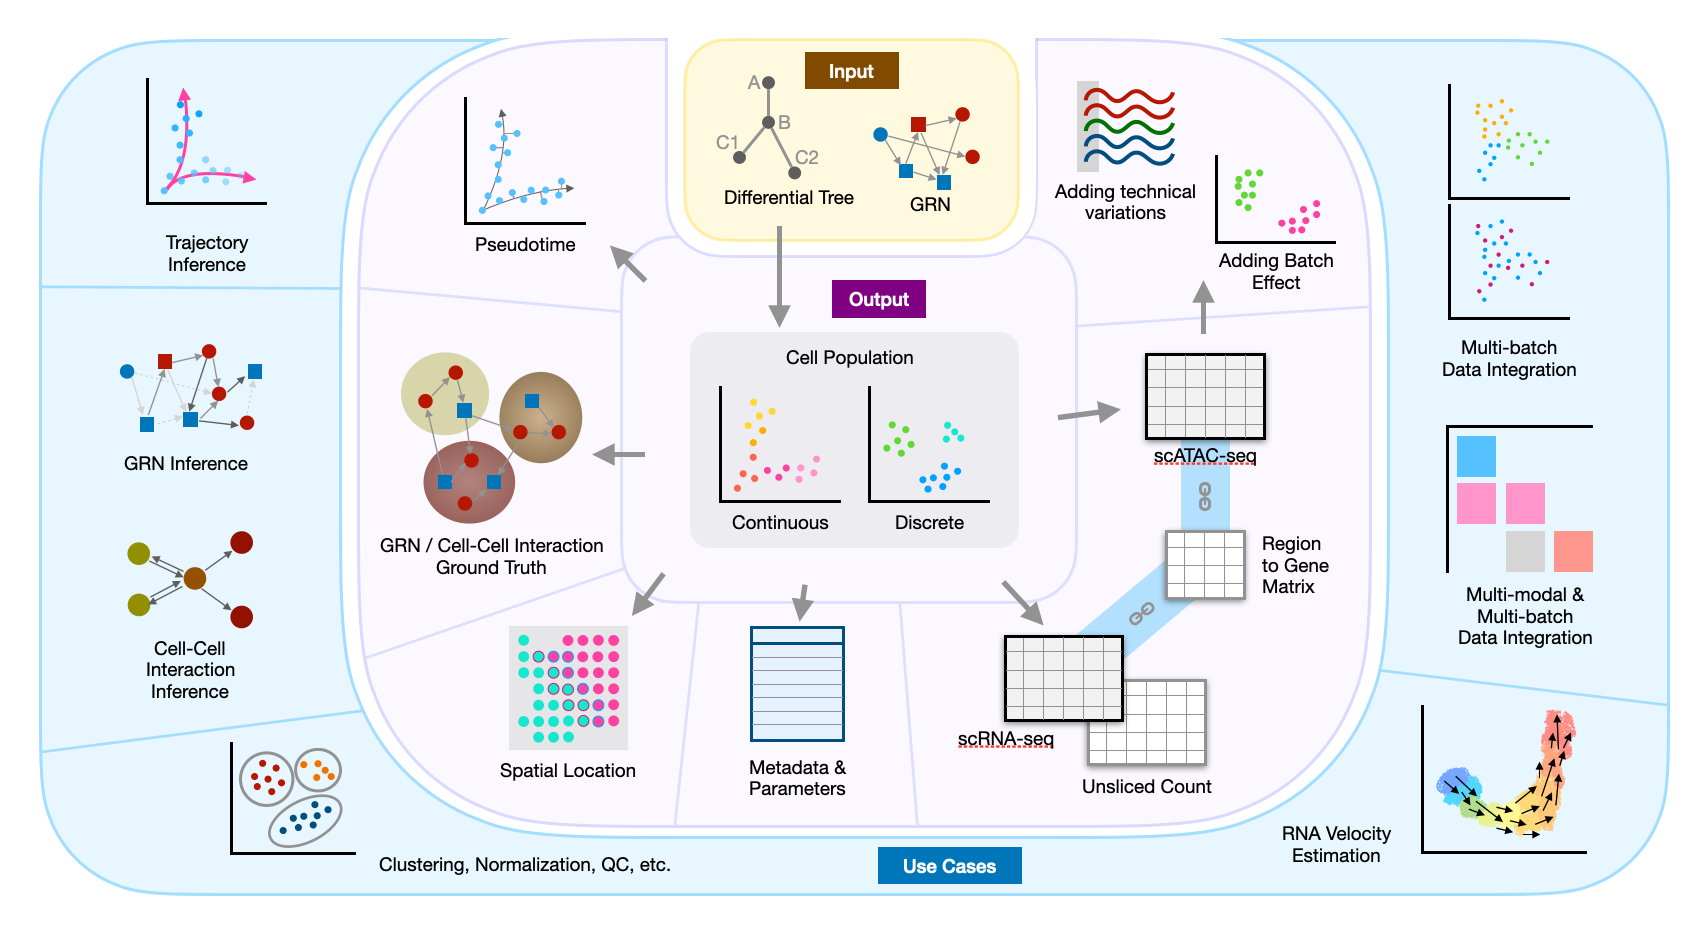
\includegraphics[width=0.85\linewidth,height=\textheight,keepaspectratio]{images/scMultisim.png}

}

\caption{\label{fig-scMultisim}Overview of \texttt{scMultiSim} from
\href{https://pmc.ncbi.nlm.nih.gov/articles/PMC10055660/figure/F1}{\textcite{li2023rs}}.
The minimal required input is a \textbf{cell differential tree}
describing the differentiation relationship of cell types, and a
user-input ground truth GRN. Optionally, a ground truth for cell-cell
interaction and technical design.}

\end{figure}%

\begin{itemize}
\tightlist
\item
  \href{SRTsim:\%20spatial\%20pattern\%20preserving\%20simulations\%20for\%20spatially\%20resolved\%20transcriptomics}{\texttt{SRTsim}},
  from \textcite{zhu2023gb}.

  \begin{itemize}
  \tightlist
  \item
    Avalaible as a
    \href{https://cran.r-project.org/web/packages/SRTsim/index.html}{CRAN
    R package}, a \href{https://github.com/xzhoulab/SRTsim}{GitHub
    repository} and a \href{https://jiaqiangzhu.shinyapps.io/srtsim}{R
    Shiny App}.
  \item
    Tutorials are avalaible
    \href{https://xzhoulab.github.io/SRTsim/02_Reference_Based_Example/}{here},
    generated using \texttt{pkgdown}.
  \item
    Three-stage simulation protocol:

    \begin{enumerate}
    \def\labelenumi{\arabic{enumi}.}
    \tightlist
    \item
      \textbf{Stage 1}: Define spatial coordinates for cell
      locations\footnote{To be paired with \texttt{spasim} which focuses
        only on spatial imaging and tissue generation, without modelling
        transcriptomic expressions.}. In details, it first uses a
      \textbf{hull} algorithm to define the \textbf{outskirt} of the
      tissue in the shape of a polygon. Secondly, within the polygon,
      you can either define a square grid within the polygon with the
      number of points determined by the user, mimmicking the process
      underlying 10X Visium generation, OR uses a random point process
      to create locations within the polygon using the
      \href{https://www.rdocumentation.org/packages/sp/versions/2.1-4/topics/spsample}{\texttt{sp::spsample}}
      R function\footnote{Underlying principle: stratified random
        sampling, quite similar to survey sampling modelling}, looking
      alike MERFISH or seqFISH+ SRT technologies.
    \item
      \textbf{Stage 2}, generate cell-specific expression counts: Four
      statistical generative models are avalaible, namely P for Poisson,
      NB for negative binomial, ZIP for zero-inflated Poisson; ZINB for
      zero-inflated negative binomial, the latter 2 accouting for model
      \textbf{zero-inflation} (the so-called \emph{drop-outs} issue
      common in scRNASeq datasets). All measures are used to infer the
      expression model for each of the 4 statistical count models
      implemented, one gene after the other (\textbf{strong assumption
      of gene independence and decorrelation with spatial location!!}).
      The model finally selected is the one exhibiting the lowest AIC,
      whose parameters are subsequently used to generate synthetic
      expression counts.
    \item
      \textbf{Step 3}: assign the simulated counts to the locations in
      the synthetic data preserving the spatial expression pattern
      observed in the reference data\footnote{Idea: instead of using
        rank-order mapping, rely on a spatial version of \textbf{optimal
        transport} for perserving distribution shape -\textgreater{}
        minimise the Wasserstein distance between real and simulated
        spatial density distributions}. Specifically, \texttt{SRTsim}
      assigns the simulated expression counts to locations in the
      synthetic data preserving the rank derived from real data (for
      instance, the spatial location associated with the highest
      expression of a given gene in the real data will match the spatial
      location assigned to synthetic data).
    \item
      \textbf{Optionnal}: Without prior knowledge, a reference-free
      simulation is also provided with the simulator, with the
      possibility of customising spatial patterns from a predefined
      shape of interest and generate synthetic data with user-specified
      model parameters.
    \item
      \textbf{Optionnal 2}: possibility to extrapolate existing domain
      areas to uncovered spatial areas using an \textbf{affine
      transformation} which preserves most of the topological features.
      Report to Figure~\ref{fig-SRTsim} below for details.
    \end{enumerate}
  \end{itemize}
\item
  \textbf{Output}: a S4 object that contains:

  \begin{itemize}
  \tightlist
  \item
    One matrix with the spatial tissue coordinates
  \item
    The corresponding simulated expression counts for all genes across
    all locations.
  \item
    The estimated model parameters, the user-defined parameter inputs
    and the input random seed.
  \end{itemize}
\end{itemize}

\begin{figure}

\centering{

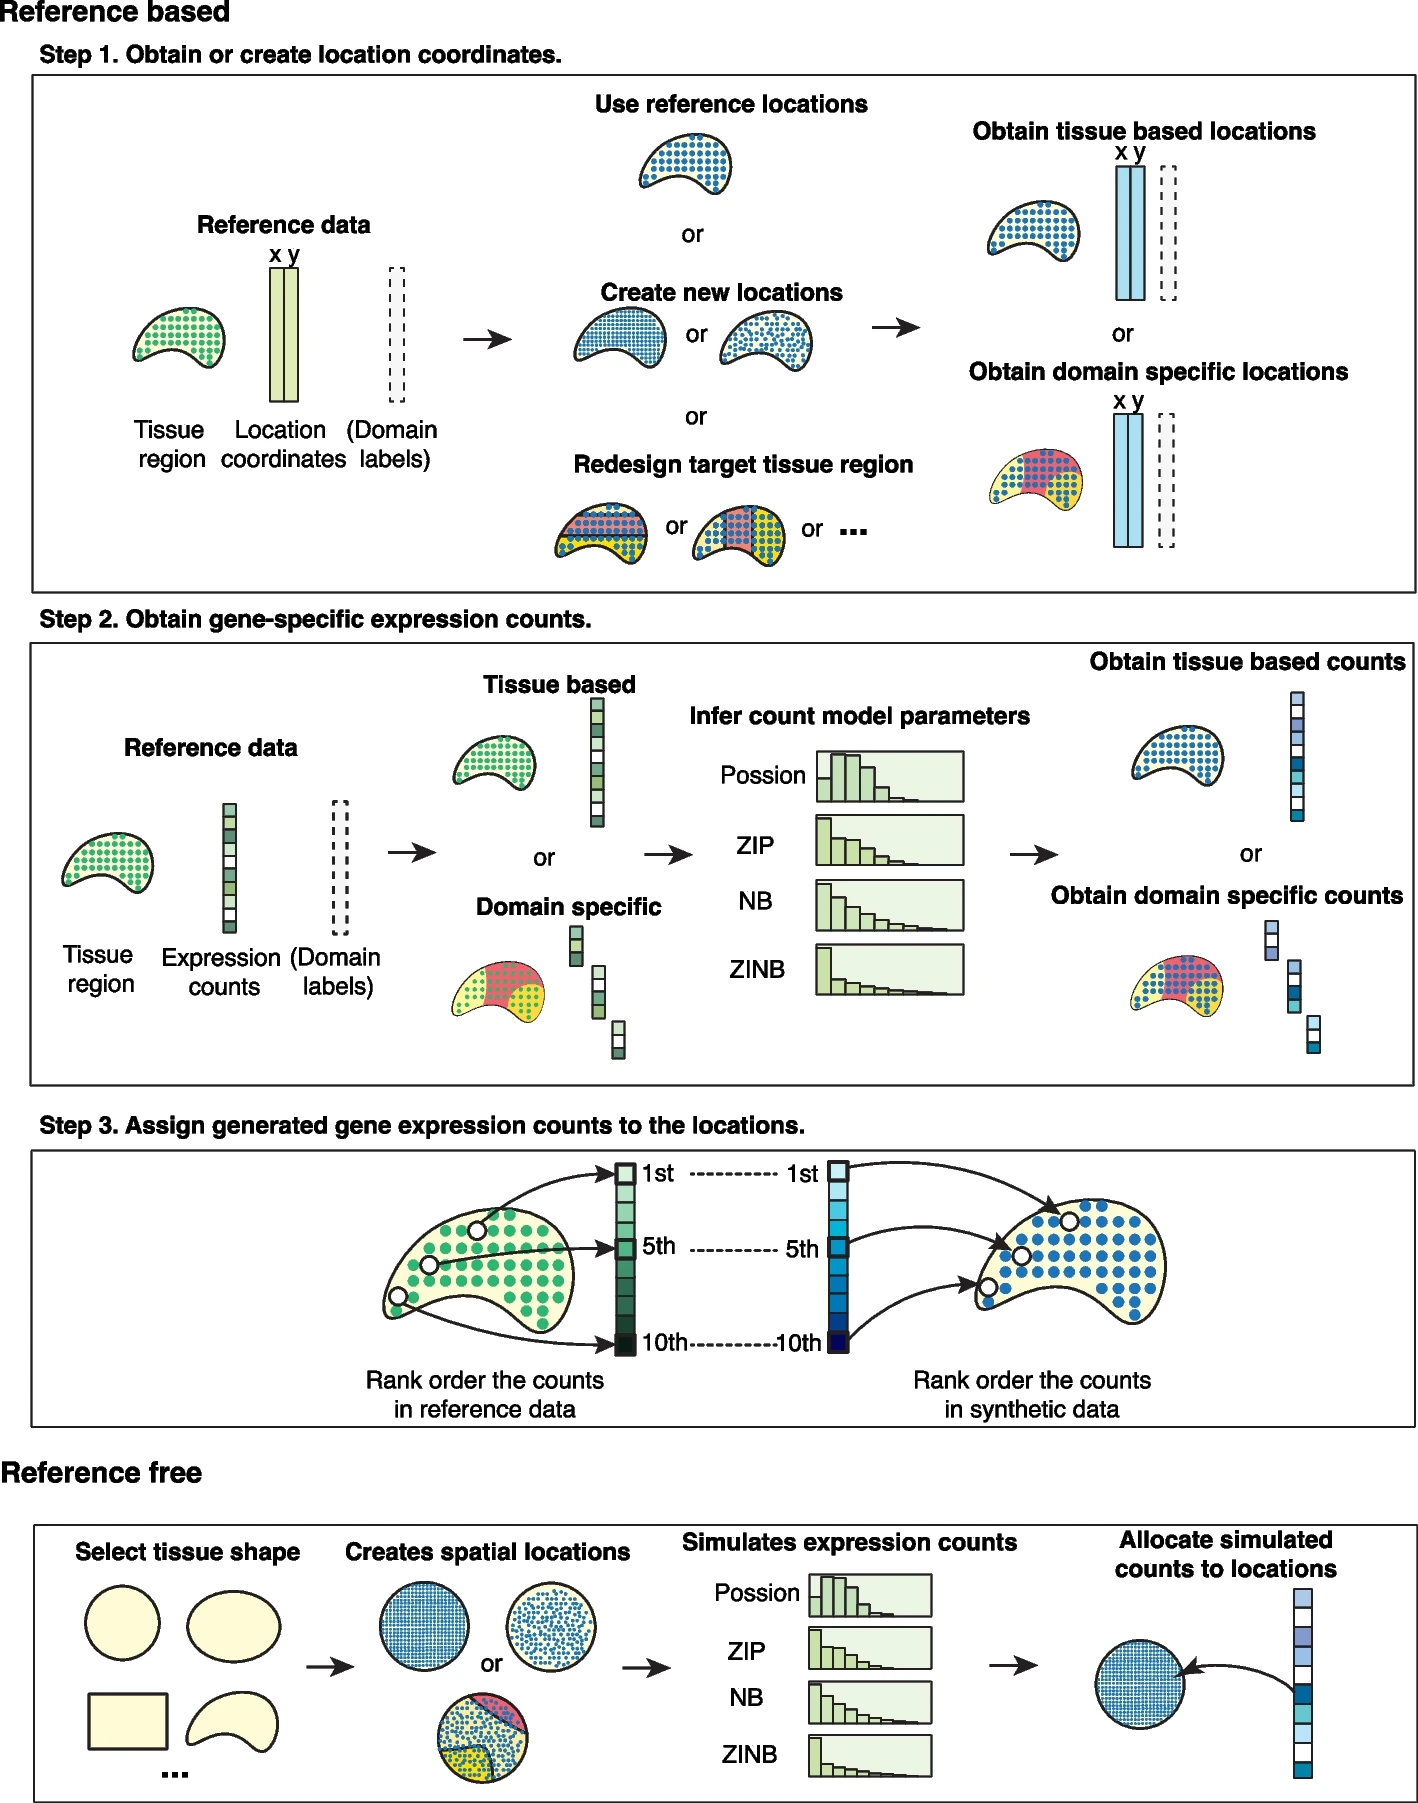
\includegraphics[width=0.85\linewidth,height=\textheight,keepaspectratio]{images/SRTsim.png}

}

\caption{\label{fig-SRTsim}Overview of \texttt{SRTsim} from
\href{https://genomebiology.biomedcentral.com/articles/10.1186/s13059-023-02879-z/figures/1}{\textcite{zhu2023gb},
Fig 1}. Inputs for the \emph{reference-based} approach include a gene
expression count matrix, a location matrix, and an optional domain
annotation matrix to depict tissue distributions.}

\end{figure}%

\subsubsection{Evaluation against ground truth
estimates}\label{evaluation-against-ground-truth-estimates}

\begin{itemize}
\tightlist
\item
  Correlation between CCC predictions and spatial adjacency
\item
  Recovering the effect of receptor gene knockouts
\item
  Robustness to subsampling
\item
  Agreement with proteomics
\item
  scRNA-Seq simulated datasets
\item
  Ground truth among methods.
\end{itemize}

\subsection{Computational platform and
paper}\label{computational-platform-and-paper}

\begin{itemize}
\tightlist
\item
  R or Python
\item
  Nextflow or Snakemake (if you start from raw datasets, or requires
  combining distinct script languages paired with slurm intensive use.)
\item
  Package structure, including \texttt{./vignettes} folder, or simple
  call to Quarto or Jupyter Notebook documents.
\item
  Github or Gitlab repository, visibility? Contributions?
\item
  Choice of the Journal:

  \begin{itemize}
  \tightlist
  \item
    Which review? Nature? Genome Biology?
  \item
    Which tool for writing the paper? Overleaf? Shared GitHub repo? Use
    of Nature quarto extensions (Pro: generate automatically both html
    and pdf versions)
  \item
    Which library repository (shared Zotero group has my favour)
  \end{itemize}
\end{itemize}

\section{Outlooks}\label{outlooks}

\subsection{Statistical perspectives and
methods}\label{statistical-perspectives-and-methods}

\begin{itemize}
\tightlist
\item
  \href{https://research.ibm.com/publications/a-perspective-on-quantum-computing-for-analyzing-cell-cell-communication-networks}{Quantum
  computing}
\end{itemize}

\subsection{Biological perspectives}\label{biological-perspectives}

\subsection{Infra and intra-cellular}\label{infra-and-intra-cellular}

\begin{itemize}
\tightlist
\item
  Estimate bot extra- and intra- intracellular activities.
\end{itemize}

\subsubsection{Multi-scale perspective}\label{multi-scale-perspective}

\begin{itemize}
\item
  \href{https://www.biorxiv.org/content/10.1101/2023.01.03.522646v1.full.pdf}{Niche
  differential gene expression analysis in spatial transcriptomics data
  identifies context-dependent cell-cell interactions}
\item
  \textbf{Multi-scale}: Instead of considering a single-cell resolution
  consider a tissue resolution of the propagation signal

  \begin{itemize}
  \tightlist
  \item
    \texttt{Visium}: spots often capture more than one cell
  \item
    \texttt{Xenium}: already at the single cell level. However, lacks of
    depth resolution.
  \end{itemize}
\end{itemize}

\subsubsection{Cross-sample and
cross-study}\label{cross-sample-and-cross-study}

\begin{itemize}
\tightlist
\item
  Cross-sample and cross-study comparisons, under different
  environmental conditions (identify the shared and differentiated
  pathways triggered from one condition to another)
\end{itemize}

\subsubsection{Dynamic cell-cell-communication
inference}\label{dynamic-cell-cell-communication-inference}

\subsubsection{Biological use cases}\label{biological-use-cases}

\begin{itemize}
\tightlist
\item
  Wound healing
\item
  TME deconvolution and niche identification
\end{itemize}

\cleardoublepage
\phantomsection
\addcontentsline{toc}{part}{Appendices}
\appendix

\chapter*{References}\label{references}
\addcontentsline{toc}{chapter}{References}

\markboth{References}{References}

\printbibliography[heading=none]

\chapter{Tools review for inferring cell-cell-communication
interactions}\label{tools-review-for-inferring-cell-cell-communication-interactions}

\section{Identified collaborations}\label{identified-collaborations}

\subsection{ADLab Collaborators:}\label{adlab-collaborators}

\begin{itemize}
\tightlist
\item
  Marie Pier Scott-Boyer: biological expertise
\item
  Antoine Bodein: network expertise.
\end{itemize}

\subsection{External collaborators:}\label{external-collaborators}

\subsubsection{Rafael Gottardo}\label{rafael-gottardo}

\begin{itemize}
\tightlist
\item
  Suggested by Danielle Malpetti, met at the 4th Clinic Meets Data
  Science (CMDS) Symposium, in Zürich.
\item
  Second and mutual interest with pathway integration for improving
  deconvolution performances using the PLIER algorithm.
\end{itemize}

\subsubsection{Mark Robinson}\label{mark-robinson}

\begin{itemize}
\tightlist
\item
  Proficient in defining and asserting the respective pros and cons of
  several statistical spatial transcriptomics.

  \begin{itemize}
  \tightlist
  \item
    \href{https://github.com/elixir-europe-training/ELIXIR-SCO-spatial-omics}{Elixir
    Spatial statistics}, provided in Figure~\ref{fig-mark-robinson}.
  \end{itemize}
\end{itemize}

\begin{figure}

\centering{

}

\caption{\label{fig-mark-robinson}}

\end{figure}%

\begin{itemize}
\item
  Strong proficiency in developing robust benchmark's architecture:

  \begin{itemize}
  \tightlist
  \item
    \href{https://omnibenchmark.org/}{Omnibenchmark repository}
  \item
    \href{https://arxiv.org/pdf/2409.17038}{Omnibenchmark for continuous
    and open benchmarking in bioinformatics}, from
    \autocite{mallona2024}
  \item
    \href{https://arxiv.org/pdf/2409.15472}{Building a continuous
    benchmarking ecosystem in bioinformatics}, from
    \autocite{mallona2024a}
  \item
    \href{https://www.birs.ca/workshops/2023/23w5090/files/Mark\%20Robinson/Robinson_BIRS_benchmarking.pdf}{2023
    Presentation to \texttt{Single\ Cell\ Plus}}, displayed in
    Figure~\ref{fig-mark-robinson2}.
  \end{itemize}
\end{itemize}

\begin{figure}

\centering{

}

\caption{\label{fig-mark-robinson2}}

\end{figure}%

\begin{itemize}
\tightlist
\item
  Half-Canadian, half-Swiss
\item
  Already discussed with him attending one of the
  \href{https://compbiozurich.org/news/}{Zürich Compbio} meeting.
\end{itemize}

\subsubsection{Yvan Saeys}\label{yvan-saeys}

\begin{itemize}
\tightlist
\item
  Proficiency in Cell-cell-communication inference methods, as showcased
  by Elixir class Figure~\ref{fig-yvan-saeys}.
\end{itemize}

\begin{figure}

\centering{

}

\caption{\label{fig-yvan-saeys}}

\end{figure}%

\begin{itemize}
\item
  \href{https://github.com/elixir-europe-training/ELIXIR-SCO-spatial-omics/blob/main/day_4/practical_6/workdir/p6_ccc.ipynb}{Jupyter
  Notebook Tutorial on CCC}
\item
  Collaborating with Julio Saez-Rodriguez lab, and recommended by
  Professor Mark Robinson.
\end{itemize}

\subsubsection{Others}\label{others}

\begin{itemize}
\item
  Fabian Theis, with
  \href{https://www.nature.com/articles/s41587-022-01467-z}{\emph{Modeling
  intercellular communication in tissues using spatial graphs of
  cells}}'s paper, from \textcite{fischer2023nb}.
\item
  Francesca Drummer
\item
  Samuel Gunz
\item
  Martin Emons (these two contacts interplay with Mark Robinson's lab)
\item
  The latter 5 associated with the following
  \href{https://elixir-europe-training.github.io/ELIXIR-SCO-spatial-omics/schedule.html}{Elixir
  class}.
\item
  Other swiss contacts: Erik van Nimwegen in Basel, Bart Deplancke in
  Lausanne and Sven Bergmann, Pierre-Luc Germain
\item
  Other EMBL/EBI contacts: Julio Saez Rodriguez + Pablo + Martin
  Garrido-Rodriguez
\item
  Laura Cantini's team on Cell-cell communication.
\end{itemize}

\section{TODO}\label{todo}

\begin{itemize}
\tightlist
\item
  \textbf{ToDo: re-use sent email to Mark Robinson} and complete
  collaborators section.
\item
  Finalise integration of Marie-Pier, including Table of exsiting
  spatial methods + add Table on single-cell approaches.

  \begin{itemize}
  \tightlist
  \item
    Tables of methods to be set in Appendix only,
  \end{itemize}
\item
  Read reviews and benchmarks papers, add dedicated sections.
\item
  Methodological hurdles Section~\ref{sec-hurdles-benchmark}:
\item
  Modern bootstrapping/bagging methods for simulating unknow
  distributions
\item
  AI tools for automated litterature review
\item
  Add litterature citations
\item
  Add real datasets approaches.
\end{itemize}

\begin{center}\rule{0.5\linewidth}{0.5pt}\end{center}

\section{List of CCC tools}\label{sec-ccc-tools}

\section*{AI-based litterature review
tools}\label{ai-based-litterature-review-tools}
\addcontentsline{toc}{section}{AI-based litterature review tools}

\markright{AI-based litterature review tools}

Using a \textbf{ChatGPT prompt}:

\begin{quote}
``Provide me with a detailed summary of this paper, including the
methodology, main findings, and comparison to existing methodologies.''
\end{quote}


\backmatter



\end{document}
